\documentclass[11pt,a4paper]{article}

% Packages
\usepackage[margin=1in]{geometry}
\usepackage{amsmath}
\usepackage{amssymb}
\usepackage{setspace}
\usepackage{graphicx}
\usepackage{natbib}
\usepackage{booktabs}
\usepackage{longtable}
\usepackage{threeparttable}
\usepackage{array}
\usepackage{float}
\usepackage{placeins}
\usepackage{caption}
\usepackage{subcaption}
\usepackage{pdflscape}
\usepackage[hidelinks]{hyperref}
\usepackage{microtype}

\geometry{margin=1in}
\onehalfspacing
\graphicspath{{../figures/}}
\hypersetup{
  pdftitle={Transfer-Dependent Frontier Growth},
  pdfauthor={S.M. Muzammil Afroz},
  pdfsubject={Financial Programming}
}
\setlength{\parskip}{0.35em}
\setlength{\parindent}{1.2em}
\bibpunct{(}{)}{;}{a}{ }{,}
\newcolumntype{L}[1]{>{\raggedright\arraybackslash}p{#1}}
\newcolumntype{C}[1]{>{\centering\arraybackslash}p{#1}}

\begin{document}

\title{\textbf{Transfer-Dependent Frontier Growth: Structural Breaks, Inflation Dynamics, and the COVID-19 Shock in Arunachal Pradesh}}
\author{S.M. Muzammil Afroz\\
Subject: Financial Programming\\
Instructor: M. Parameswaran\\
Centre For Development Studies}
\date{April 2026}
\maketitle

\begin{abstract}
This paper studies the growth and inflation experience of Arunachal Pradesh relative to all India and a set of regional and hill-state comparators. The empirical design follows the assignment requirement: estimate trend growth in constant-price GDP and GSDP, test for structural breaks using the Bai-Perron multiple-break framework, compute kinked exponential growth rates, and construct quarterly and annual inflation measures from CPI and implicit deflators. The analysis adds three extensions: a state-comparator module, a sectoral transformation check, and a COVID-19 shock comparison. The central finding is that Arunachal Pradesh is not a simple post-1991 liberalisation acceleration case. Its constant-price GSDP breaks are dated at 1995-96 and 2013-14, not at 1987-88 statehood or the 1991 reforms. Trend growth declines from 7.63 percent in 1980-95 to 6.61 percent in 1996-2013 and 5.54 percent in 2014-24. Subperiod evidence is sharper: the pre-liberalisation CAGR is 9.34 percent, above the 5.18 percent recorded during 1991-2003. Inflation evidence shows a frontier-market pattern: Arunachal Pradesh's rural CPI inflation is slightly higher and substantially more volatile than all-India combined CPI inflation, with a particularly large fuel premium. The COVID-19 output shock was negative but not uniquely severe among comparable states; the subsequent recovery was weaker than Assam, Sikkim, Tripura, and Meghalaya. The paper interprets Arunachal Pradesh as a transfer-dependent frontier economy whose growth has been real but only weakly associated with deep industrial transformation.
\end{abstract}

\tableofcontents
\newpage

\section{Introduction}

Economic growth in India is usually narrated around two national questions: when did the long-run acceleration begin, and how much of it can be attributed to the 1991 reforms? That aggregate question is important, but it is incomplete for frontier and hill states. In states such as Arunachal Pradesh, the relevant mechanisms are not only trade liberalisation, industrial licensing, and private investment. They also include state formation, central transfers, infrastructure constraints, thin local markets, and the high transport cost of serving a sparsely populated border economy.

This paper asks whether Arunachal Pradesh's growth and inflation experience resembles the all-India growth-transition story or a more specific frontier-state path. The empirical answer is clear. Arunachal Pradesh grew rapidly, but its growth path does not look like a standard liberalisation acceleration. The Bai-Perron procedure identifies breaks in 1995-96 and 2013-14, whereas the most obvious administrative candidate, the transition to statehood in 1987-88, is not selected. Nor is 1991-92 selected as a growth break for the state. The kinked growth estimates show steady deceleration rather than acceleration: 7.63 percent in 1980-95, 6.61 percent in 1996-2013, and 5.54 percent in 2014-24. Cross-state comparisons reinforce the result. Arunachal Pradesh's pre-1991 CAGR is 9.34 percent, while its 1991-2003 CAGR is only 5.18 percent.

The second part of the paper studies inflation. Arunachal Pradesh's CPI data are rural-only, so the state series is not directly symmetric with all-India combined CPI. Even with this limitation, the pattern is informative. Quarterly rural CPI inflation in Arunachal Pradesh averages 5.90 percent, compared with 5.58 percent for all India, but its standard deviation is much higher. The annual evidence shows large swings: headline inflation is 12.12 percent in 2012-13, 8.91 percent in 2018-19, falls sharply in 2019-20, and then normalises after the pandemic. A cross-state CPI comparison shows that Arunachal Pradesh's mean headline inflation over the available period is close to Tripura and Assam, while its fuel inflation is persistently elevated.

The contribution is therefore both descriptive and interpretive. Descriptively, the paper produces a complete analysis of all-India GDP, Arunachal Pradesh GSDP, CPI inflation, deflator inflation, headline inflation, and core inflation. Interpretively, it argues that Arunachal Pradesh is best read as a transfer-dependent frontier economy rather than a state that followed the all-India liberalisation cycle. The evidence does not deny growth; it changes the explanation of growth. Output expanded, but the timing of breaks, sectoral composition, and inflation volatility point to a state whose macroeconomic performance is shaped by public expenditure, terrain, logistics, and a narrow productive base.

\section{Literature Review}

The analysis is grounded in four strands of literature. The first studies growth as a sequence of regimes rather than a single average. \citet{hausmann_pritchett_rodrik_2004} define growth accelerations as sustained departures from prior trends, while \citet{bai_perron_1998,bai_perron_2003} provide the econometric framework for estimating multiple unknown breaks in linear models. \citet{zeileis_leisch_hornik_kleiber_2002} document the \textit{strucchange} implementation used in applied work. Once breaks are identified, a simple segmented regression is not ideal for trend-growth estimation because it permits discontinuous jumps in log output. The kinked exponential model of \citet{boyce_1986} imposes continuity and interprets breaks as changes in growth rates.

The second strand concerns India's growth transition. \citet{rodrik_subramanian_2005} argue that India's growth shift began before 1991, whereas \citet{agarwal_whalley_2013} caution against a mechanical attribution of growth acceleration to the reforms alone. \citet{balakrishnan_parameswaran_2007} similarly emphasise the importance of careful growth-rate estimation in the Indian context. This debate matters for Arunachal Pradesh because a post-1991 acceleration should not be assumed; it must be tested against the state series.

The third strand studies regional growth and convergence among Indian states. \citet{sachs_bajpai_ramiah_2002} show that regional growth depends on structural conditions, while \citet{bhattacharya_sakthivel_2004}, \citet{bandyopadhyay_2011}, and \citet{sodsriwiboon_kalra_2010} document divergence, polarisation, club formation, and weak spillovers among Indian states. The recent public-finance evidence in \citet{govil_chauhan_2024} is especially relevant because Arunachal Pradesh's growth cannot be separated from fiscal capacity and central transfers. This literature motivates the comparator set used here: Assam as a Northeast regional baseline, Sikkim as a small Himalayan benchmark, Himachal Pradesh as a hill-state counterfactual outside the Northeast, and Tripura and Meghalaya as additional Northeast comparators.

The fourth strand studies spatial inflation and the COVID-19 shock. \citet{kundu_kishore_bhoi_2018} and \citet{jha_dhal_2019} show that regional inflation dispersion persists even under a common national monetary policy, especially through food and supply-side channels. \citet{mahajan_tomar_2021} and \citet{narayanan_saha_2021} document the food-supply disruption caused by the pandemic, while \citet{beyer_francobedoya_galdo_2021} show that the COVID-19 economic shock varied across Indian states. These studies are directly relevant for Arunachal Pradesh because terrain, distance from major supply centres, and the thinness of local markets can amplify food and fuel price volatility.

\section{Data}

The output data come from the EPW Research Foundation India Time Series. All-India GDP is observed at current and constant prices from 1950-51 to 2025-26. Arunachal Pradesh GSDP is observed at current and constant prices from 1980-81 to 2024-25. The assignment requirement is fully covered; the latest available observations are retained where available. Arunachal Pradesh data prior to statehood should be read as the economic series of the territory that became the state, not as evidence of an independent state government's policy regime.

Monthly CPI data are available from January 2011 to December 2025. All-India CPI is available for rural, urban, and combined sectors with major subgroups. Arunachal Pradesh CPI is available only for the rural sector. Its urban CPI is missing for all major groups, and the sporadic combined values are identical to rural values where reported. Therefore all state-level CPI calculations use Arunachal Pradesh rural CPI. This is not a discretionary choice; it follows from the source data.

Core inflation is computed with the inclusion method. For all India, the core index is constructed from clothing and footwear, housing, and miscellaneous components using the available rural and urban weights. For Arunachal Pradesh, housing is not available in the rural CPI basket, so core inflation uses clothing and footwear and miscellaneous only. The state core measure is therefore narrower and should be interpreted as an indicative non-food, non-fuel inflation measure rather than a perfectly comparable all-India core index. The distortion is not trivial: housing carries zero weight in rural CPI but 21.67 points in the all-India urban core basket used here.

The state-comparator module uses long-run all-state GSDP, NSDP, and CPI data. Table \ref{tab:data-summary} summarises the main series. The chosen comparators are not arbitrary. Assam is the natural regional benchmark; Sikkim captures the small-Himalayan high-growth case; Himachal Pradesh provides a hill-state comparison outside the Northeast; Tripura and Meghalaya add robustness within the Northeast.

\begin{table}[H]
\centering
\caption{Main data sources and coverage}
\label{tab:data-summary}
\begin{threeparttable}
\small
\begin{tabular}{L{2.8cm}L{4.7cm}L{2.8cm}L{2.9cm}}
\toprule
Series & Source and unit & Period used & Main limitation \\
\midrule
All-India GDP & GDP at current and constant prices, Rs crore & 1950-51 to 2025-26 & Latest years are provisional/revised where applicable \\
Arunachal Pradesh GSDP & GSDP at current and constant prices, Rs lakh converted as needed & 1980-81 to 2024-25 & Pre-1987 observations refer to the territory before statehood \\
All-India CPI & CPI 2012=100, monthly, major groups & Jan. 2011 to Dec. 2025 & Core construction uses available CPI groups and weights \\
Arunachal Pradesh CPI & CPI 2012=100, monthly, rural major groups & Jan. 2011 to Dec. 2025 & Urban CPI is absent; combined CPI is not usable \\
Comparator states & All-state GSDP/NSDP backseries and state CPI & varies by state & Sikkim has no pre-1991 GSDP sample \\
\bottomrule
\end{tabular}
\begin{tablenotes}
\footnotesize
\item Notes: The annual inflation table reports the required 2011-12 to 2023-24 window and retains 2024-25 as the latest available extension. Arunachal Pradesh CPI in 2020-21 is affected by missing April and May 2020 observations.
\end{tablenotes}
\end{threeparttable}
\end{table}

\section{Methodology}

The baseline growth equation is
\begin{equation}
\ln Y_t = \alpha + \beta t + u_t,
\end{equation}
where $Y_t$ is real GDP or real GSDP and $\beta$ is the instantaneous trend growth rate. The compound annual growth rate is computed as
\begin{equation}
\mathrm{CAGR} = \left(e^\beta - 1\right)\times 100.
\end{equation}
Structural breaks are estimated using the Bai-Perron multiple-break framework with up to five breaks and a trimming parameter of 0.10, with model selection by the Bayesian information criterion (Bai and Perron 1998; Bai and Perron 2003; Zeileis et al. 2002).

When breaks are detected, growth is estimated using a kinked exponential model:
\begin{equation}
\ln Y_t = \alpha + \beta_1 t + \sum_{j=1}^{m}\delta_j(t-T_j)D_{jt} + u_t,
\end{equation}
where $T_j$ is the $j$th break date and $D_{jt}=1$ if $t>T_j$. The post-break regime-$j$ growth coefficient is therefore $\beta_1+\delta_j$. The specification permits the slope to change at a break while maintaining continuity in the level of log output. This is appropriate for trend-growth estimation because structural breaks in growth need not imply jumps in the level of output (Boyce 1986). Heteroskedasticity-robust standard errors and bootstrap confidence intervals are used for inference.

This continuity-constrained pooled regression is close in spirit to the segment-by-segment kinked-trend tradition, but it is not identical in inferential structure. Under fixed break dates and an imposed continuity restriction, the pooled specification reproduces the same broken-line fitted path as a piecewise trend written segment by segment; what changes is that all regime slopes are estimated jointly and discrete level shifts at the break dates are ruled out by construction. The bootstrap intervals reported here should therefore be read as uncertainty around a continuous-growth-path parametrisation rather than as tests for discontinuous jumps in log output.

The COVID-19 shock is studied in two ways. First, a 2020-21 pulse dummy is added to the growth model:
\begin{equation}
\ln Y_t = \alpha + \beta_1 t + \sum_{j=1}^{m}\delta_j(t-T_j)D_{jt} + \gamma \,\mathbf{1}\{t=2020\text{--}21\} + u_t.
\end{equation}
Second, a more transparent realised-shock metric compares actual real GSDP growth from 2019-20 to 2020-21 with the pre-COVID trend from 2014-15 to 2019-20:
\begin{equation}
\mathrm{Shock}_s = g^{\mathrm{actual}}_{s,\,2019\text{--}20 \rightarrow 2020\text{--}21} - g^{\mathrm{trend}}_{s,\,2014\text{--}15 \rightarrow 2019\text{--}20}.
\end{equation}
The post-COVID recovery CAGR is computed as
\begin{equation}
\mathrm{Recovery\ CAGR}_s = \left(\frac{Y_{s,\mathrm{latest}}}{Y_{s,2020\text{--}21}}\right)^{1/n_s}-1,
\end{equation}
where $n_s$ is the number of years between 2020-21 and the latest available observation for state $s$. The realised-shock metric is used for cross-state comparisons because it is easy to interpret and less dependent on the parametric break specification.

For price indices, monthly observations are first mapped into Indian fiscal years, where April--June is Q1, July--September is Q2, October--December is Q3, and January--March is Q4. Let $I_{s,g,m}$ denote the CPI index for state or sector $s$, item group $g$, and month $m$. The fiscal-quarter average is
\begin{equation}
\bar I_{s,g,fq} = \frac{1}{N_{s,g,fq}}\sum_{m \in fq} I_{s,g,m},
\end{equation}
where $N_{s,g,fq}$ is the number of observed months in that fiscal quarter. Quarterly CPI inflation is then computed year-on-year as
\begin{equation}
\pi^{Q}_{s,g,fq} = \left(\frac{\bar I_{s,g,fq}}{\bar I_{s,g,fq-4}} - 1\right)\times 100.
\end{equation}

Fiscal-year CPI averages are constructed as
\begin{equation}
\bar I_{s,g,f} = \frac{1}{M_{s,g,f}}\sum_{m \in f} I_{s,g,m},
\end{equation}
where $M_{s,g,f}$ is the number of observed months in fiscal year $f$. Annual headline inflation is
\begin{equation}
\pi^{H}_{s,f} = \left(\frac{\bar I_{s,\mathrm{general},f}}{\bar I_{s,\mathrm{general},f-1}} - 1\right)\times 100.
\end{equation}
Food and fuel inflation are computed analogously by replacing the general index with the food or fuel group average.

Core inflation follows the inclusion method described below. For all India, the monthly rural core index is
\begin{equation}
C^{R}_{m} = \frac{7.36\,I^{R}_{\mathrm{cloth},m} + 27.26\,I^{R}_{\mathrm{misc},m}}{34.62},
\end{equation}
the monthly urban core index is
\begin{equation}
C^{U}_{m} = \frac{5.57\,I^{U}_{\mathrm{cloth},m} + 21.67\,I^{U}_{\mathrm{housing},m} + 29.53\,I^{U}_{\mathrm{misc},m}}{56.77},
\end{equation}
and the combined all-India monthly core index is
\begin{equation}
C^{AI}_{m} = \frac{0.5462\times 34.62\,C^{R}_{m} + 0.4538\times 56.77\,C^{U}_{m}}{0.5462\times 34.62 + 0.4538\times 56.77}.
\end{equation}
This is a population-weighted rural-urban core index, renormalised within the core basket rather than the full CPI basket. The corresponding annual all-India core inflation rate is
\begin{equation}
\pi^{C}_{AI,f} = \left(\frac{\bar C^{AI}_{f}}{\bar C^{AI}_{f-1}} - 1\right)\times 100,
\qquad
\bar C^{AI}_{f} = \frac{1}{12}\sum_{m \in f} C^{AI}_{m}.
\end{equation}

For Arunachal Pradesh, urban CPI is unavailable and housing is absent from the rural CPI basket. The monthly state core index is therefore
\begin{equation}
C^{AR}_{m} = \frac{6.44\,I^{R}_{\mathrm{cloth},m} + 24.70\,I^{R}_{\mathrm{misc},m}}{31.14},
\end{equation}
and annual state core inflation is
\begin{equation}
\pi^{C}_{AR,f} = \left(\frac{\bar C^{AR}_{f}}{\bar C^{AR}_{f-1}} - 1\right)\times 100,
\qquad
\bar C^{AR}_{f} = \frac{1}{M^{C}_{AR,f}}\sum_{m \in f} C^{AR}_{m}.
\end{equation}
In the estimation procedure, India fiscal-year core is retained only when all 12 months are present; Arunachal Pradesh fiscal-year core is retained when the available-month count is sufficient to preserve the chain, which leaves 2020-21 in the sample with an explicit caveat. In the Arunachal Pradesh CPI workbook, duplicate all-missing general-index rows appear in early 2013; these rows are dropped before monthly merges so that annual core inflation is not mechanically distorted by duplicated months.

Deflator-based inflation is computed from the ratio of current-price to constant-price output:
\begin{equation}
P^{D}_{t} = 100\times \frac{Y^{N}_{t}}{Y^{R}_{t}},
\end{equation}
where $Y^{N}_{t}$ is current-price GDP or GSDP and $Y^{R}_{t}$ is constant-price GDP or GSDP. At the annual frequency, deflator inflation is recorded as the log difference
\begin{equation}
\pi^{D,A}_{t} = 100\left(\ln P^{D}_{t} - \ln P^{D}_{t-1}\right).
\end{equation}

Because quarterly GSDP is not directly observed for Arunachal Pradesh, annual current-price and constant-price GSDP are temporally disaggregated separately with the `tempdisagg` implementation
\begin{equation}
\texttt{td}(Y_t \sim 1,\ \texttt{to = ``quarterly''},\ \texttt{method = ``denton-cholette''}),
\end{equation}
that is, Denton-Cholette interpolation without a high-frequency indicator, using a constant preliminary series (Sax and Steiner 2013). In the unifying notation of Sax and Steiner, the quarterly estimate is
\begin{equation}
\hat{\mathbf y} = \mathbf p + D_{DC}\left(\mathbf y_l - C\mathbf p\right),
\end{equation}
where $\mathbf y_l$ is the annual series, $C$ is the annual-summing conversion matrix, $\mathbf p$ is the constant preliminary quarterly series, and $D_{DC}$ is the Denton-Cholette distribution matrix. The essential accounting restriction is
\begin{equation}
C\hat{\mathbf y} = \mathbf y_l,
\end{equation}
equivalently,
\begin{equation}
\sum_{q \in t}\hat y_q = Y_t \quad \text{for each fiscal year } t.
\end{equation}
Operationally, this produces a smooth quarterly path that exactly preserves annual benchmarks while avoiding the initial transient movement associated with the original Denton procedure (Dagum and Cholette 2006; Sax and Steiner 2013). After interpolation, the quarterly deflator is
\begin{equation}
P^{D}_{q} = 100\times \frac{\hat Y^{N}_{q}}{\hat Y^{R}_{q}},
\end{equation}
and quarterly deflator inflation is computed year-on-year as
\begin{equation}
\pi^{D,Q}_{q} = \left(\frac{P^{D}_{q}}{P^{D}_{q-4}} - 1\right)\times 100.
\end{equation}

\section{Growth Results}

Table \ref{tab:breaks} reports the structural break dates. All-India GDP has four breaks under the baseline trimming parameter: 1971-72, 1978-79, 2003-04, and 2018-19. The result is consistent with the view that India's growth transition is not reducible to a single 1991 break. For Arunachal Pradesh, the estimated breaks are 1995-96 and 2013-14. Neither 1987-88 nor 1991-92 is selected. This is one of the paper's central empirical results.

The break dates also need an economic reading. The 1995-96 break is best interpreted as a mid-1990s transition within a public-investment and administrative-catch-up growth model rather than as a single reform event. Official Northeast policy documents for 1995-96 emphasised roads, power projects, and region-building institutions under the North Eastern Council, which is consistent with a frontier economy whose growth depended heavily on public expenditure and connectivity support rather than on private industrial take-off \citep{mha_1996_annual_report,cashin_sahay_1995}. The 2013-14 break is easier to read as the onset of a slower regime. It lines up with the later comparator evidence, where Assam, Sikkim, and Tripura outperform Arunachal Pradesh after 2013, and with a sectoral pattern in which services remain dominant while industry stays modest \citep{niti_ncaer_2025_arunachal}. A plausible mechanism is the mid-decade shift in the transfer regime itself: the Fourteenth Finance Commission moved more resources into untied devolution even as it explicitly noted the North-eastern states' heavy dependence on central transfers for capital expenditure and infrastructure \citep{fourteenth_finance_commission_2015}. For a state such as Arunachal Pradesh, that kind of shift could preserve revenues while weakening the project-specific growth impulse that earlier plan-style and infrastructure-linked support had provided. In that sense, the two breaks point to regime shifts inside the same frontier-state development model: first from early catch-up to slower transfer-supported growth, and then from that phase to a still slower post-2013 regime.

The extra all-India breaks also require interpretation. The short 1971-72 to 1978-79 regime is best read as a disturbed interval rather than as a fully separate long-run epoch. It is a seven-year low-growth segment located between the pre-1971 trend and the post-1978 recovery, and it plausibly captures the macroeconomic turbulence around the Bangladesh war, the first oil shock, and the weakening of the early Green Revolution impulse. That segment disappears once trimming is raised above 0.10, so the economically sensible reading is that the baseline specification is allowed to isolate a short transitional slowdown that more conservative trimming rules absorb into the broader pre-1979 period. This is a plausible reason why the present paper finds four breaks while more aggregated accounts of India's growth transition often emphasise only the later 1978-79 and 2003-04 turning points.

The 2018-19 break is easier to interpret as the consolidation of the late-2010s national slowdown. Its timing is more consistent with the cumulative effects of demonetisation, GST transition costs, NBFC stress, and weakening investment demand than with a single one-year event. In this annual sample, those frictions appear to cumulate into a distinct lower-growth regime only by 2018-19, which is why the break is dated later than in some shorter-window studies that place the slowdown closer to the middle of the decade.

\begin{table}[H]
\centering
\caption{Bai-Perron structural break results}
\label{tab:breaks}
\small
\begin{tabular}{L{3.1cm}C{1.1cm}C{2.6cm}C{2.6cm}L{3.2cm}}
\toprule
Series & Breaks & Break 1 & Break 2 & Additional breaks \\
\midrule
All-India GDP & 4 & 1971 [1969, 1972] & 1978 [1976, 1979] & 2003 [2002, 2004]; 2018 [2016, 2019] \\
Arunachal Pradesh GSDP & 2 & 1995 [1994, 1996] & 2013 [2012, 2014] & none \\
\bottomrule
\end{tabular}
\end{table}

The kinked growth estimates in Table \ref{tab:growth-regimes} translate the break dates into regime growth rates. All-India GDP growth rises from 3.88 percent in 1950-71 to 5.53 percent in 1979-2003 and 6.92 percent in 2004-18, before moderating to 4.93 percent in the post-2018 regime. Arunachal Pradesh shows the opposite shape. Its trend growth rate is highest in the first regime, at 7.63 percent, then declines to 6.61 percent and 5.54 percent. The state therefore grows rapidly, but the evidence is of gradual deceleration rather than post-reform acceleration.

\begin{table}[H]
\centering
\caption{Kinked exponential trend growth rates}
\label{tab:growth-regimes}
\begin{tabular}{L{2.7cm}C{2.3cm}C{1.8cm}C{1.8cm}C{2.5cm}C{2cm}}
\toprule
Series & Period & $\beta$ & CAGR & Bootstrap 95\% CI & Years \\
\midrule
All-India & 1950-1971 & 0.03802 & 3.88 & [3.74, 4.00] & 22 \\
All-India & 1972-1978 & 0.02476 & 2.51 & [2.02, 3.01] & 7 \\
All-India & 1979-2003 & 0.05378 & 5.53 & [5.36, 5.68] & 25 \\
All-India & 2004-2018 & 0.06694 & 6.92 & [6.65, 7.17] & 15 \\
All-India & 2019-2025 & 0.04808 & 4.93 & [2.91, 5.55] & 7 \\
Arunachal Pradesh & 1980-1995 & 0.07352 & 7.63 & [6.98, 8.15] & 16 \\
Arunachal Pradesh & 1996-2013 & 0.06403 & 6.61 & [6.19, 7.06] & 18 \\
Arunachal Pradesh & 2014-2024 & 0.05395 & 5.54 & [5.04, 6.33] & 11 \\
\bottomrule
\end{tabular}
\end{table}

The subperiod comparison in Table \ref{tab:comparators-growth} makes the interpretation more concrete. Arunachal Pradesh grows at 9.34 percent during 1980-91, much faster than Assam, Himachal Pradesh, Tripura, and Meghalaya. During 1991-2003, however, its growth falls to 5.18 percent. The state does grow faster again during 2003-13, but the post-2013 regime slows to 5.58 percent, below Assam, Sikkim, and Tripura. This trajectory does not fit a simple liberalisation story. It is closer to a frontier-state path where early public investment, administrative consolidation, and transfers created rapid growth from a low base, but without a later manufacturing-led transformation.

\begin{table}[H]
\centering
\caption{Comparator-state real GSDP growth by period}
\label{tab:comparators-growth}
\begin{tabular}{L{3.4cm}C{2.2cm}C{2.2cm}C{2.2cm}C{2.2cm}}
\toprule
State & 1980-1991 & 1991-2003 & 2003-2013 & 2013-latest \\
\midrule
Arunachal Pradesh & 9.34 & 5.18 & 7.45 & 5.58 \\
Assam & 4.17 & 3.01 & 4.89 & 7.71 \\
Sikkim & n.a. & 6.54 & 13.55 & 7.47 \\
Himachal Pradesh & 4.51 & 6.45 & 7.87 & 5.23 \\
Tripura & 5.42 & 7.67 & 8.33 & 7.44 \\
Meghalaya & 5.87 & 5.49 & 7.13 & 4.34 \\
\bottomrule
\end{tabular}
\begin{flushleft}
\footnotesize Notes: Entries are compound annual growth rates in percent. Sikkim has no pre-1991 constant-price GSDP sample in the available data. Latest year is 2024 for all listed states except Sikkim, where it is 2023.
\end{flushleft}
\end{table}

\begin{figure}[H]
\centering
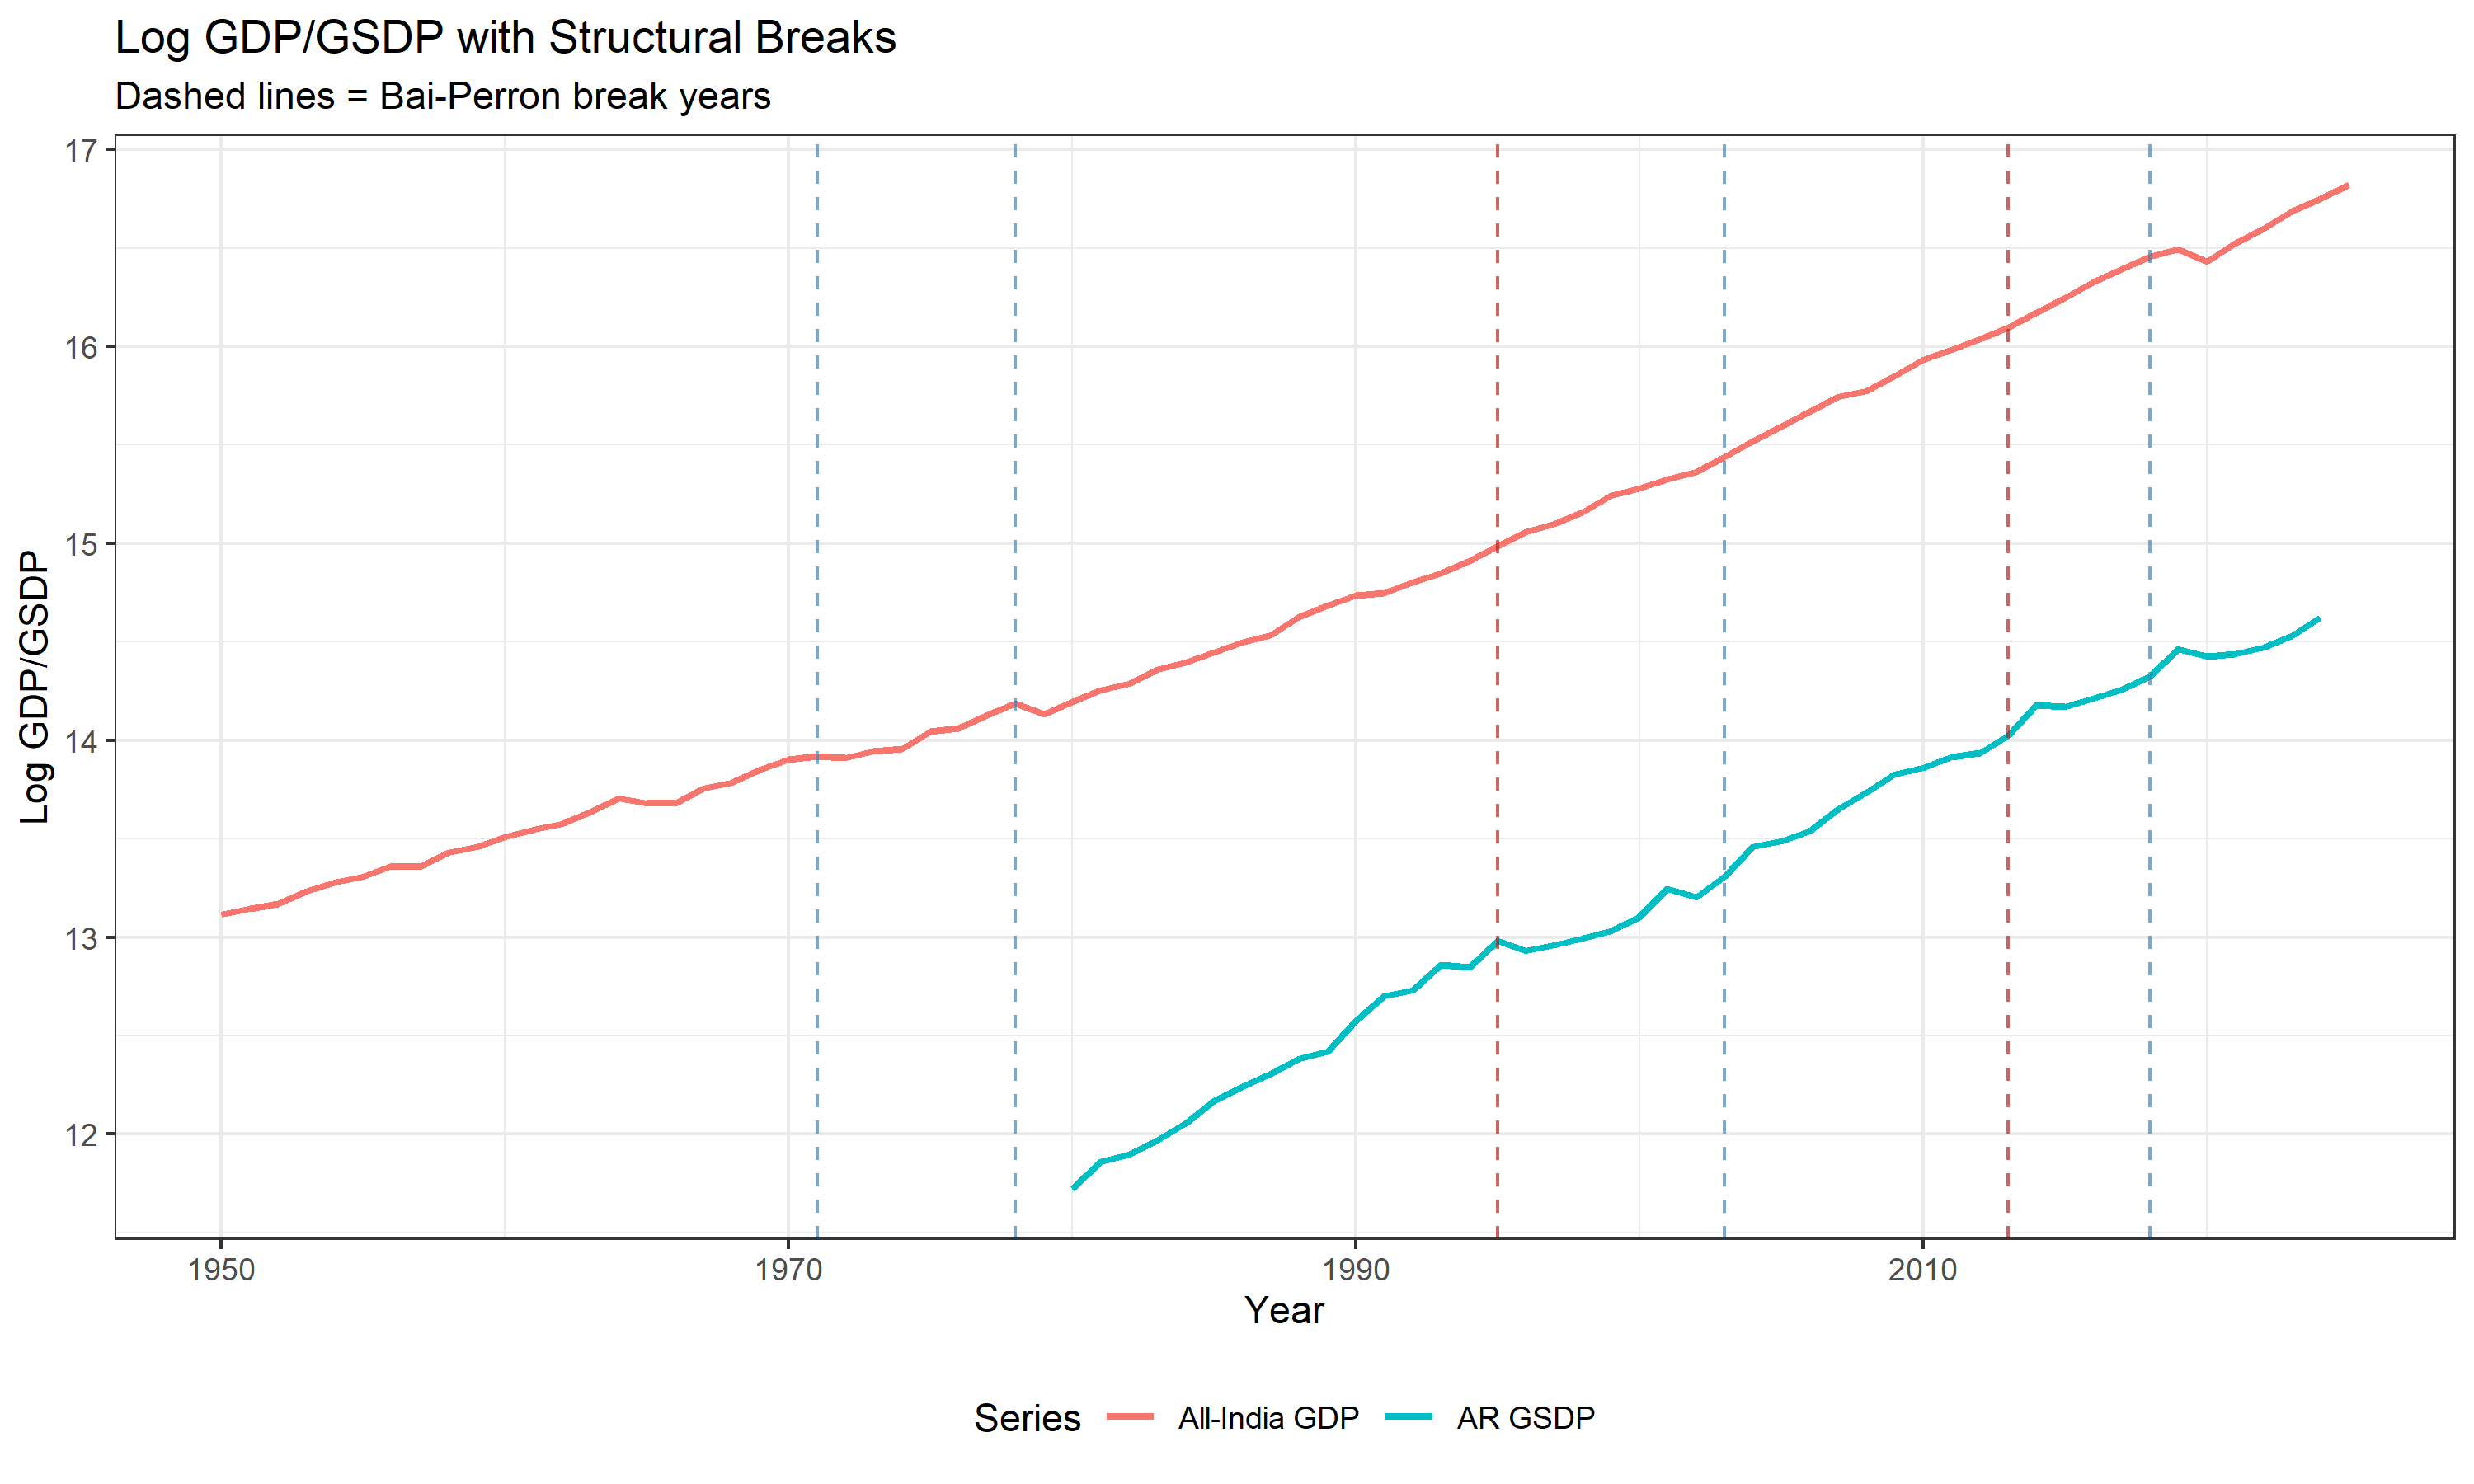
\includegraphics[width=0.92\textwidth]{fig1_log_gdp_breaks.png}
\caption{All-India log real GDP with estimated structural breaks}
\label{fig:india-breaks}
\end{figure}

\begin{figure}[H]
\centering
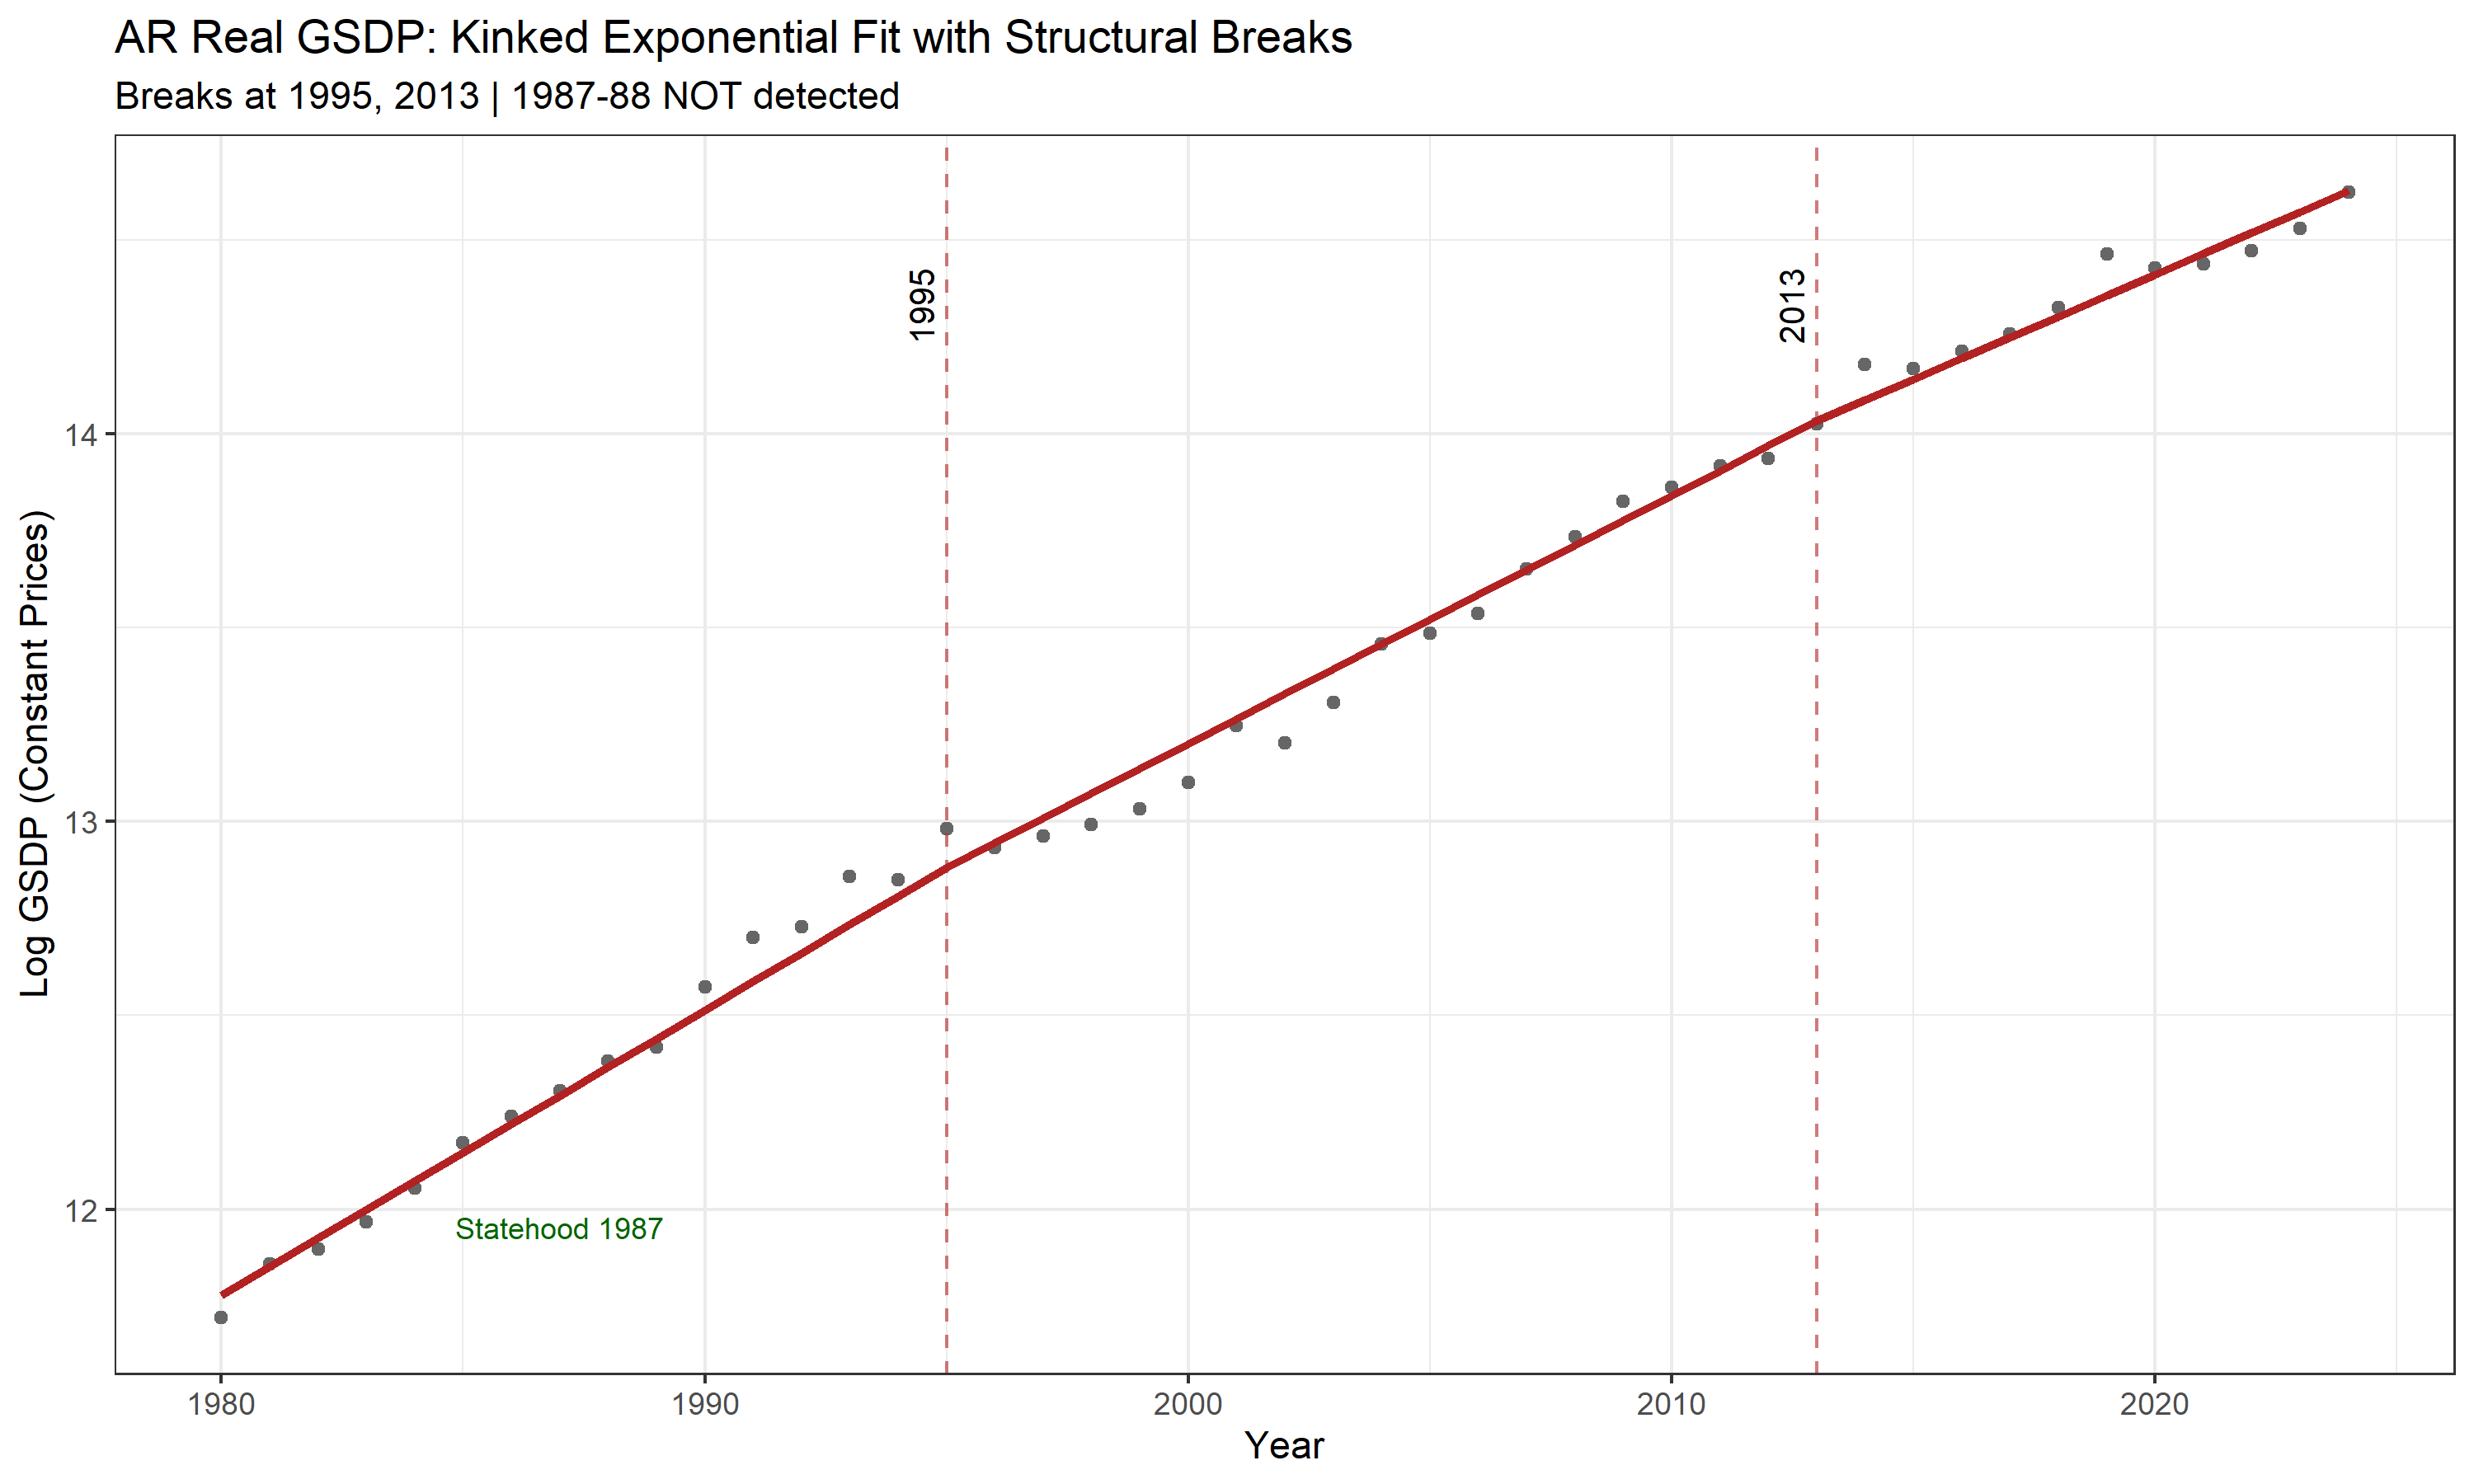
\includegraphics[width=0.92\textwidth]{fig2_ar_gsdp_breaks.png}
\caption{Arunachal Pradesh log real GSDP with estimated structural breaks}
\label{fig:ar-breaks}
\end{figure}

\FloatBarrier

\section{Structural Transformation}

The growth results raise a natural question: if Arunachal Pradesh grew rapidly, what changed inside the economy? The sectoral evidence in Figure \ref{fig:sectoral} points to growth without deep industrial transformation. Agriculture's share declines over the long run, but the space is absorbed mainly by services rather than by a large and durable industrial expansion. By 2024-25, services account for nearly half of constant-price GSDP, while industry remains modest. This pattern resembles India's broader services-led development path discussed by \citet{kochhar_kumar_rajan_subramanian_tokatlidis_2006}, but in Arunachal Pradesh the relevant service expansion is more plausibly tied to public administration, construction-linked services, transfers, and infrastructure spending than to large-scale private tradable services.

This distinction matters for interpretation. A growth acceleration caused by industrialisation would normally leave signs in the sectoral composition: a rising industrial share, higher labour absorption outside agriculture, and stronger productivity spillovers. Arunachal Pradesh's evidence is weaker on these dimensions. The state grows, but the composition suggests that the growth process remains fiscally and administratively mediated.

\begin{figure}[H]
\centering
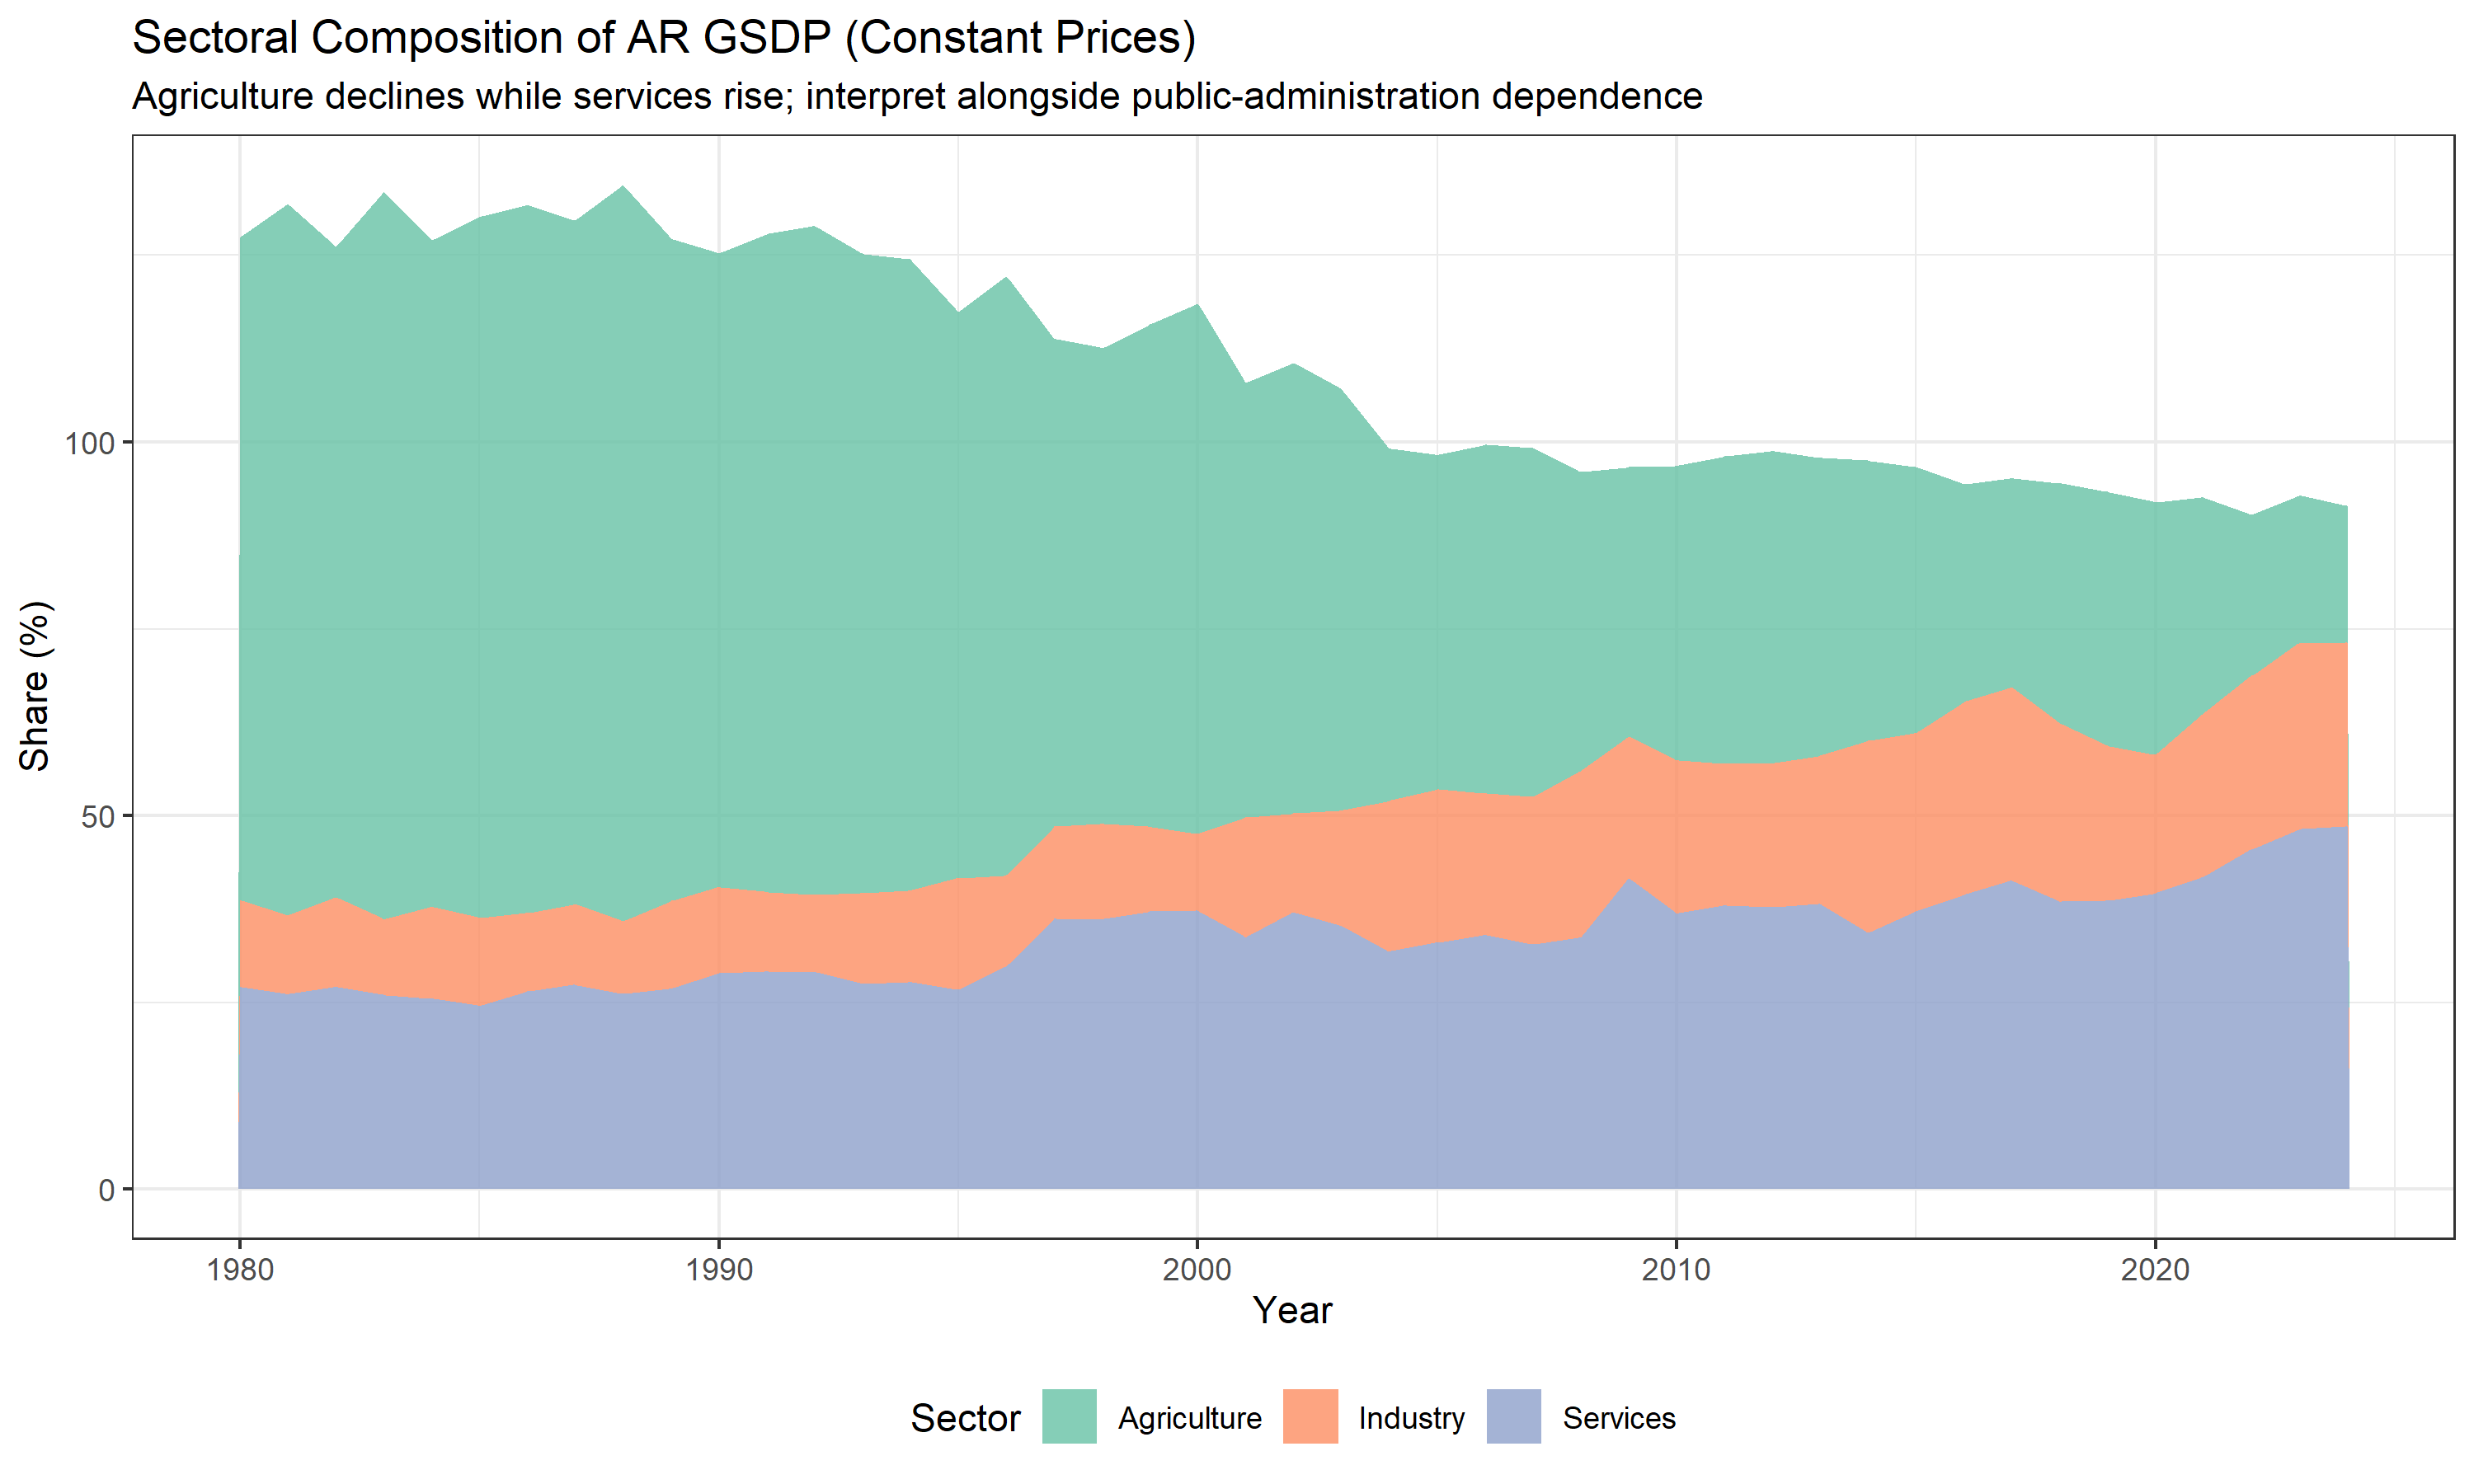
\includegraphics[width=0.92\textwidth]{fig3_sectoral_shares.png}
\caption{Sectoral shares in Arunachal Pradesh GSDP}
\label{fig:sectoral}
\end{figure}

\section{Inflation Results}

Table \ref{tab:quarterly-stats} reports summary statistics for quarterly inflation. Arunachal Pradesh rural CPI inflation averages 5.90 percent, slightly above all-India combined CPI inflation at 5.58 percent. The more important difference is volatility. The standard deviation of Arunachal Pradesh quarterly CPI inflation is 3.34, compared with 2.28 for all India. Deflator-based inflation for Arunachal Pradesh is still more volatile, but that result should be read carefully because quarterly GSDP is interpolated from annual benchmarks.

\begin{table}[H]
\centering
\caption{Quarterly inflation summary statistics}
\label{tab:quarterly-stats}
\begin{tabular}{L{3cm}C{3cm}C{3cm}C{3cm}}
\toprule
Statistic & AR rural CPI & India combined CPI & AR GSDP deflator \\
\midrule
Mean & 5.90 & 5.58 & 6.91 \\
Median & 6.01 & 5.27 & 5.95 \\
Standard deviation & 3.34 & 2.28 & 4.34 \\
Minimum & -2.15 & 0.76 & -0.56 \\
Maximum & 13.05 & 10.59 & 21.24 \\
Number of quarters & 56 & 56 & 176 \\
\bottomrule
\end{tabular}
\end{table}

The time-series pattern in Figure \ref{fig:quarterly-cpi} is consistent with the regional inflation literature. Arunachal Pradesh inflation is not permanently disconnected from the national series, but deviations can be large. The pre-COVID period shows a positive mean premium of 1.22 percentage points. In the COVID and post-COVID period, the premium turns negative on average, partly because all-India inflation remained elevated while Arunachal Pradesh's measured rural headline inflation fell during the pandemic data gap and then normalised.

\begin{figure}[H]
\centering
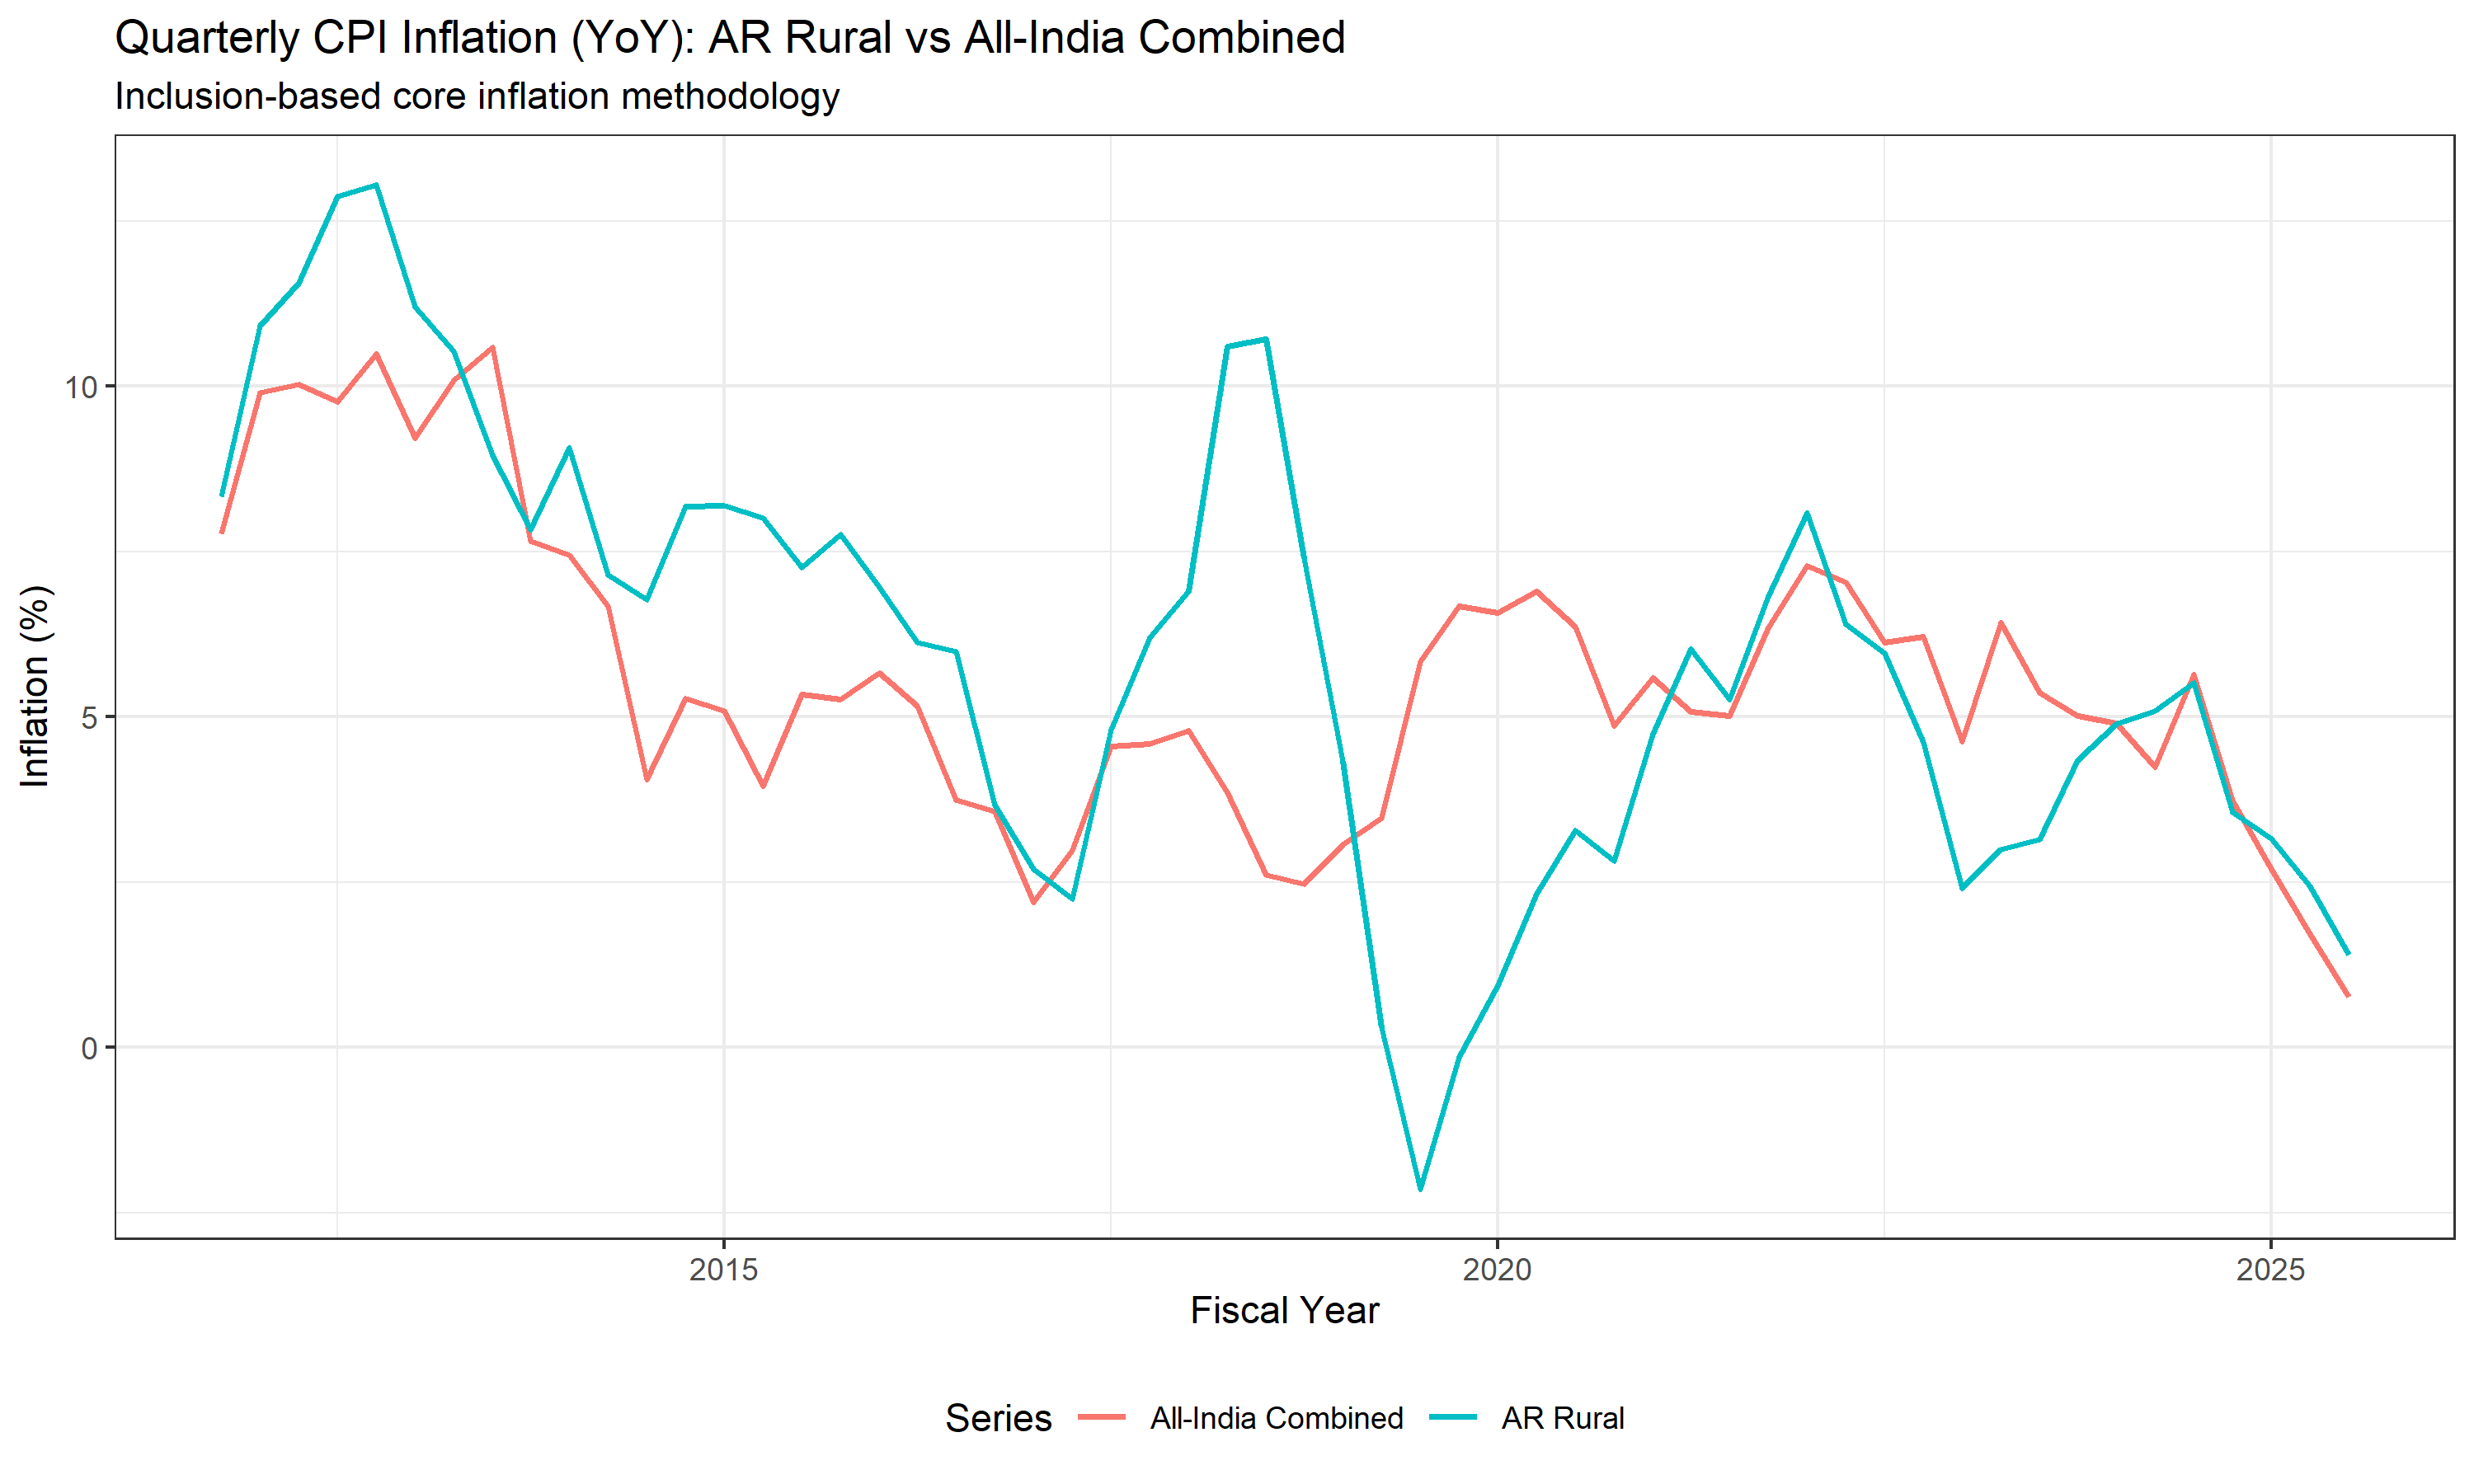
\includegraphics[width=0.92\textwidth]{fig5_quarterly_cpi.png}
\caption{Quarterly CPI inflation: Arunachal Pradesh rural and all-India combined}
\label{fig:quarterly-cpi}
\end{figure}

Annual headline and core inflation are shown in Figure \ref{fig:headline-core} and in full in Appendix Table \ref{tab:annual-inflation}. The annual inflation window begins effectively in 2012-13 because a year-on-year fiscal-year rate for 2011-12 would require a full 2010-11 monthly CPI baseline, which is not available in the source panel. Arunachal Pradesh headline inflation is 12.12 percent in 2012-13 and 8.91 percent in 2018-19, compared with 10.05 and 3.41 percent respectively for all India. In 2020-21, the Arunachal Pradesh headline series sits well below the all-India rate, but this year must be read with caution because April and May 2020 are missing in the Arunachal Pradesh CPI data. By 2024-25, headline inflation is similar in the two series: 4.76 percent for Arunachal Pradesh and 4.63 percent for all India.

The core comparison needs a more explicit quantitative caveat. Arunachal Pradesh has only a rural CPI and no housing component, whereas housing carries 21.67 urban weight points in the national CPI and 9.83 points, or 22.0 percent, in the population-weighted combined national core basket. Appendix Table \ref{tab:inflation-diagnostics} therefore reports a sensitivity check in which housing is removed from the national urban core as well. Over 2012-13 to 2024-25, that adjustment changes annual all-India core inflation by 0.29 percentage points on average in absolute value, with a maximum effect of 0.71 points in 2021-22. The sign is not one-sided, because housing inflation sometimes runs below and sometimes above the rest of the core basket. The implication is that the state-national core comparison is imperfect but still informative: the housing omission is large enough to matter for fine year-by-year reading, but not large enough to overturn the paper's broader inflation ranking.

\begin{figure}[H]
\centering
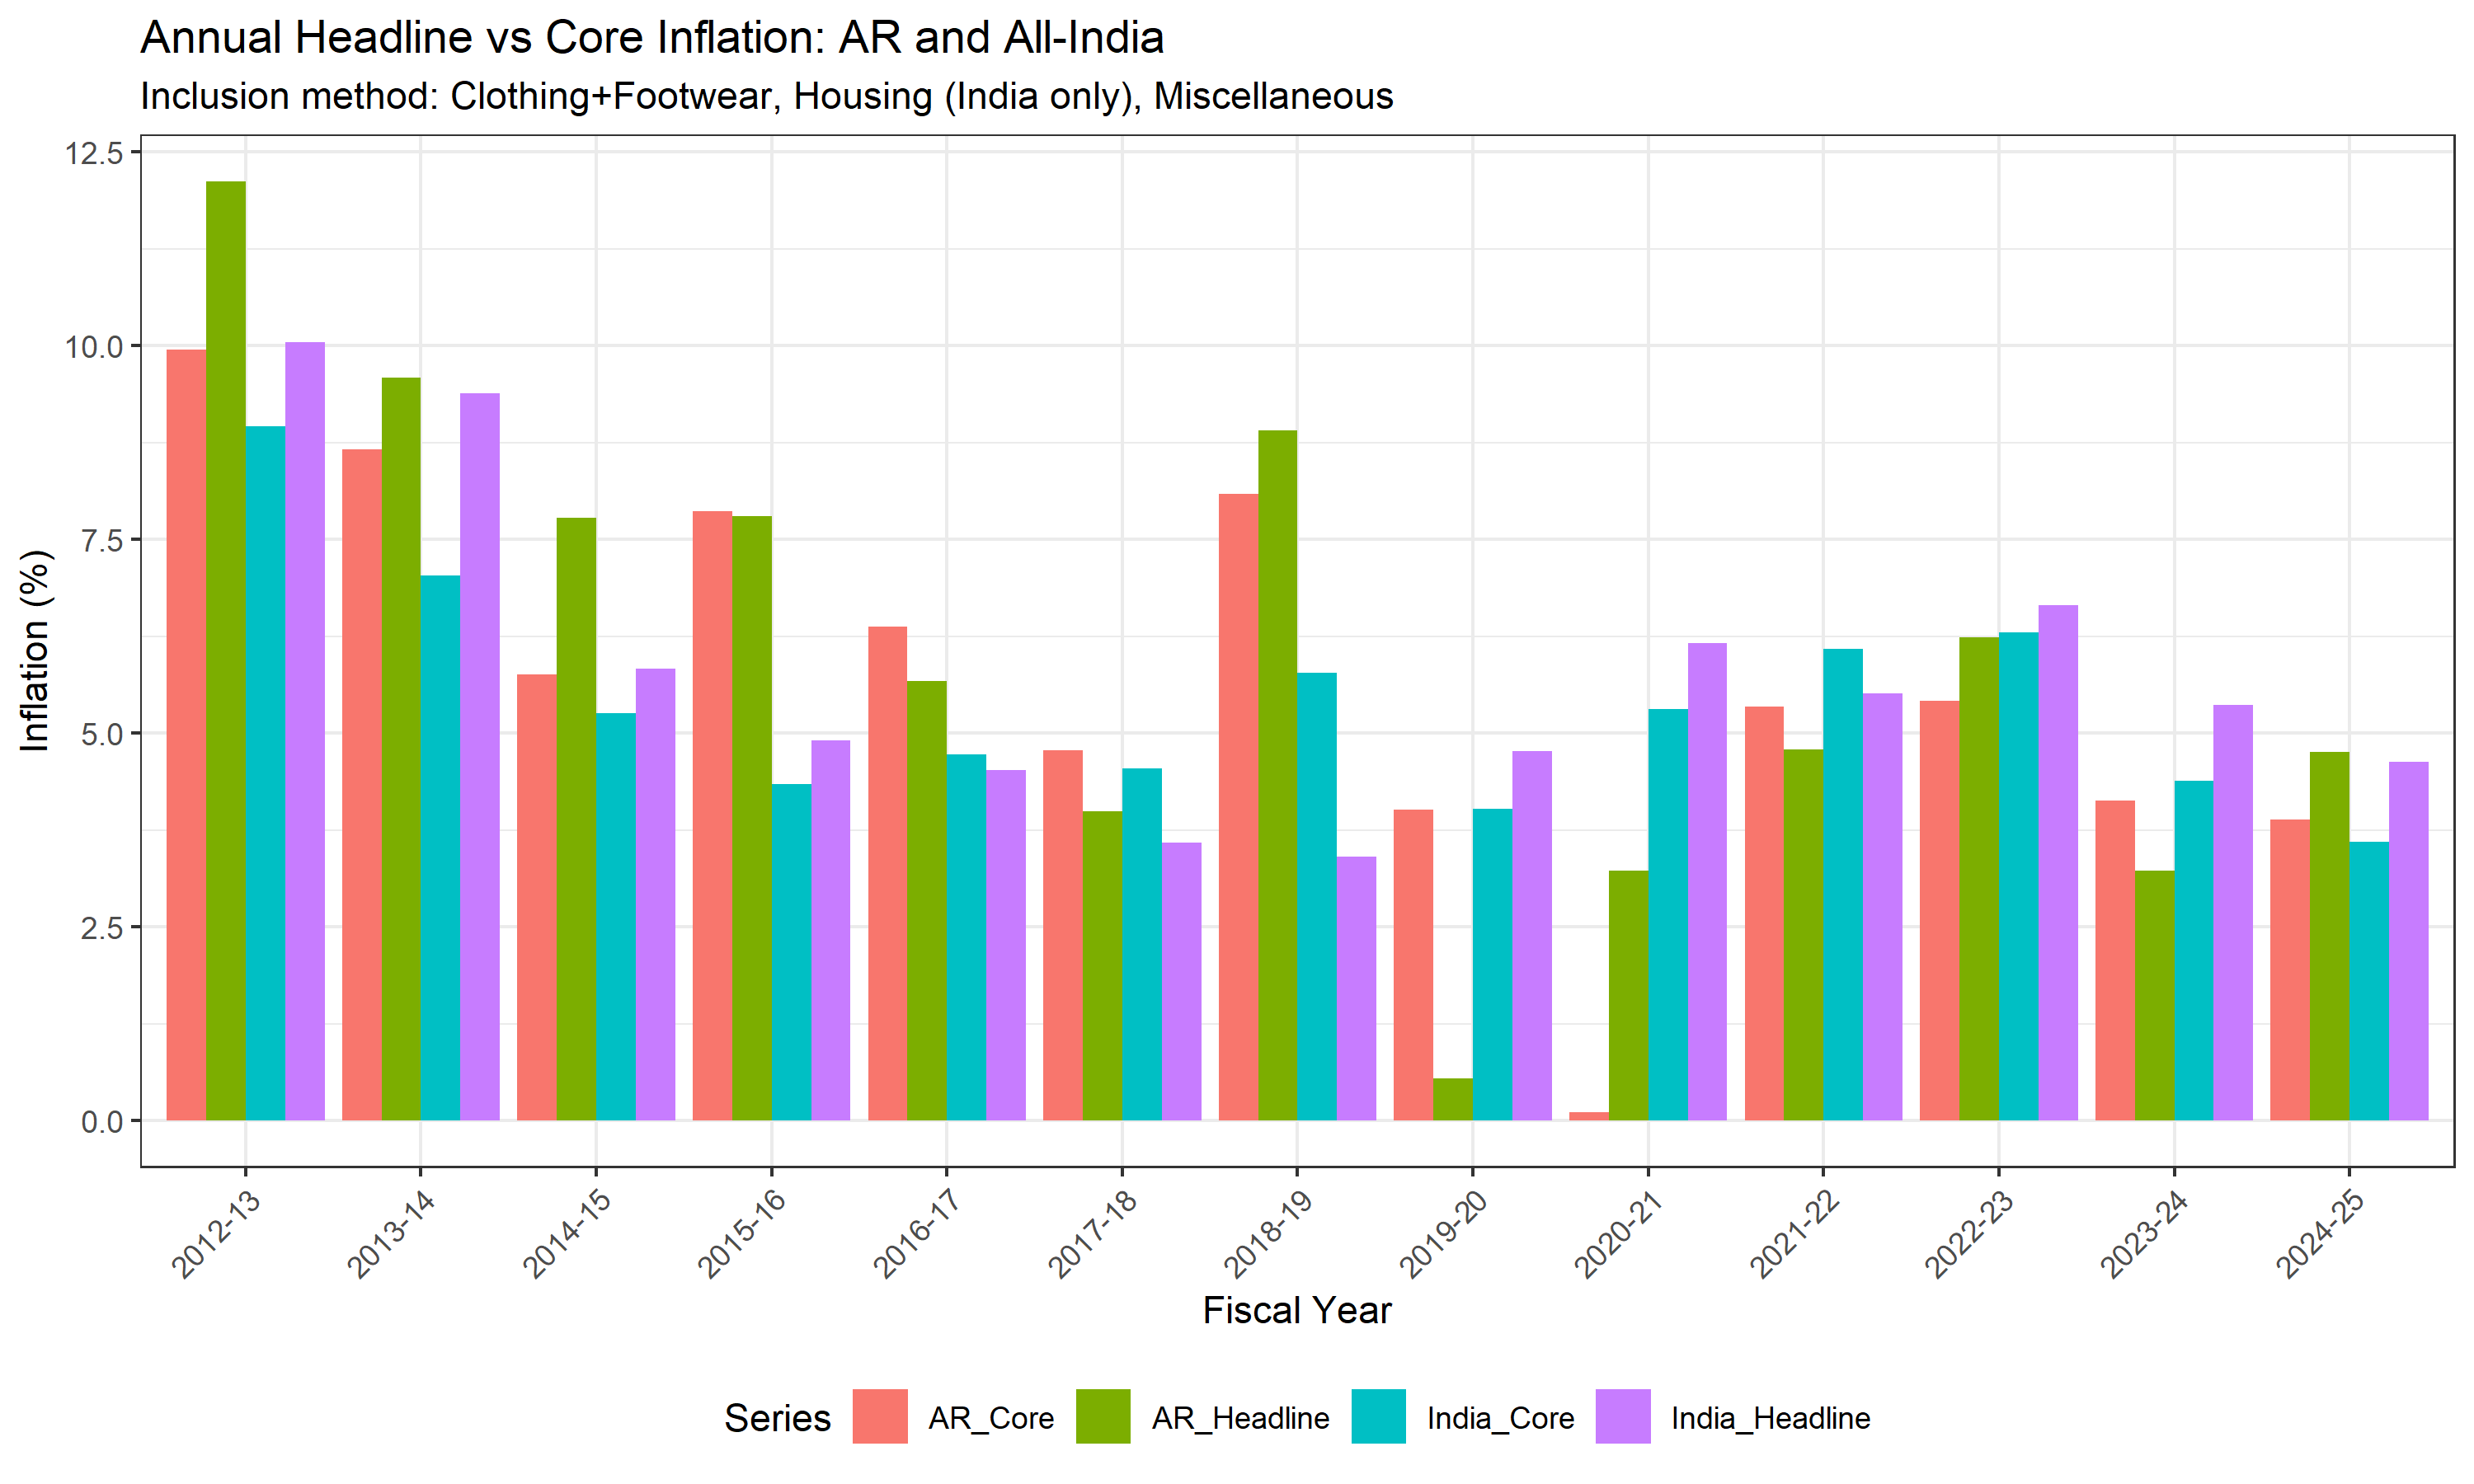
\includegraphics[width=0.92\textwidth]{fig6_headline_core.png}
\caption{Annual headline and core inflation}
\label{fig:headline-core}
\end{figure}

The cross-state CPI comparison in Table \ref{tab:cpi-comparison} shows that Arunachal Pradesh is not an outlier in mean headline inflation among Northeast comparators. Its mean headline inflation, 6.05 percent, is close to Tripura and Assam. Its fuel inflation, however, is high: 7.54 percent on average, compared with 5.11 percent for all India and 3.42 percent for Himachal Pradesh. That result deserves separate attention rather than a passing logistics-cost remark.

The degree of national co-movement is also measurable rather than impressionistic. The Pearson correlation between quarterly year-on-year Arunachal Pradesh rural headline inflation and all-India combined headline inflation is 0.54 over the 56-quarter overlap, with $p<0.001$; Appendix Table \ref{tab:inflation-diagnostics} reports the formal test. The state is therefore not disconnected from the national inflation cycle. What distinguishes it is partial rather than zero integration: co-movement is positive, but far from one-for-one, volatility is higher, and the fuel premium remains persistently positive. The same table also shows that the correlation is strong before COVID-19 and much weaker after 2020, which is consistent with pandemic-era supply distortions and the temporary Arunachal Pradesh data gap.

Figure \ref{fig:fuel-premium} shows that Arunachal Pradesh's annual fuel inflation premium over all India is positive in most years. The premium averages roughly 3.0 percentage points in 2012-13 to 2018-19 and 2.6 points in 2021-22 to 2024-25, so it narrows slightly after the pandemic but does not disappear. The same-year correlation between Arunachal Pradesh fuel inflation and Arunachal Pradesh headline inflation is 0.61, whereas the one-year lead correlation is close to zero. The evidence therefore supports a contemporaneous cost-pass-through reading more strongly than a clean leading-indicator story: when fuel prices spike in the state, headline inflation tends to move with them in the same year. This is exactly what one would expect in a thin, high-transport-cost market where fuel is an input into retail distribution as much as a household purchase item. The pandemic year should again be read cautiously because missing months depress the state series mechanically.

\begin{table}[H]
\centering
\caption{Cross-state CPI pressure, 2012-13 to 2024-25}
\label{tab:cpi-comparison}
\begin{tabular}{L{3.4cm}C{2.1cm}C{2.1cm}C{2.1cm}C{2.1cm}}
\toprule
State & Headline mean & Headline SD & Food mean & Fuel mean \\
\midrule
All India & 5.75 & 1.97 & 6.16 & 5.11 \\
Arunachal Pradesh & 6.05 & 3.16 & 5.87 & 7.54 \\
Assam & 5.87 & 2.14 & 5.75 & 8.12 \\
Himachal Pradesh & 5.20 & 2.36 & 5.47 & 3.42 \\
Meghalaya & 5.34 & 3.68 & 5.34 & 7.11 \\
Sikkim & 5.83 & 2.20 & 6.07 & 7.98 \\
Tripura & 6.06 & 3.33 & 5.79 & 8.84 \\
\bottomrule
\end{tabular}
\begin{flushleft}
\footnotesize Notes: Entries are annual inflation rates in percent. Arunachal Pradesh uses rural CPI; other states use combined CPI where available. Headline, food, and fuel inflation are read directly from the published combined CPI group indices. Exact combined-state core CPI is not reported because the state weight file supplies rural and urban basket weights, but not a state-specific combined basket weight vector.
\end{flushleft}
\end{table}

\begin{figure}[H]
\centering
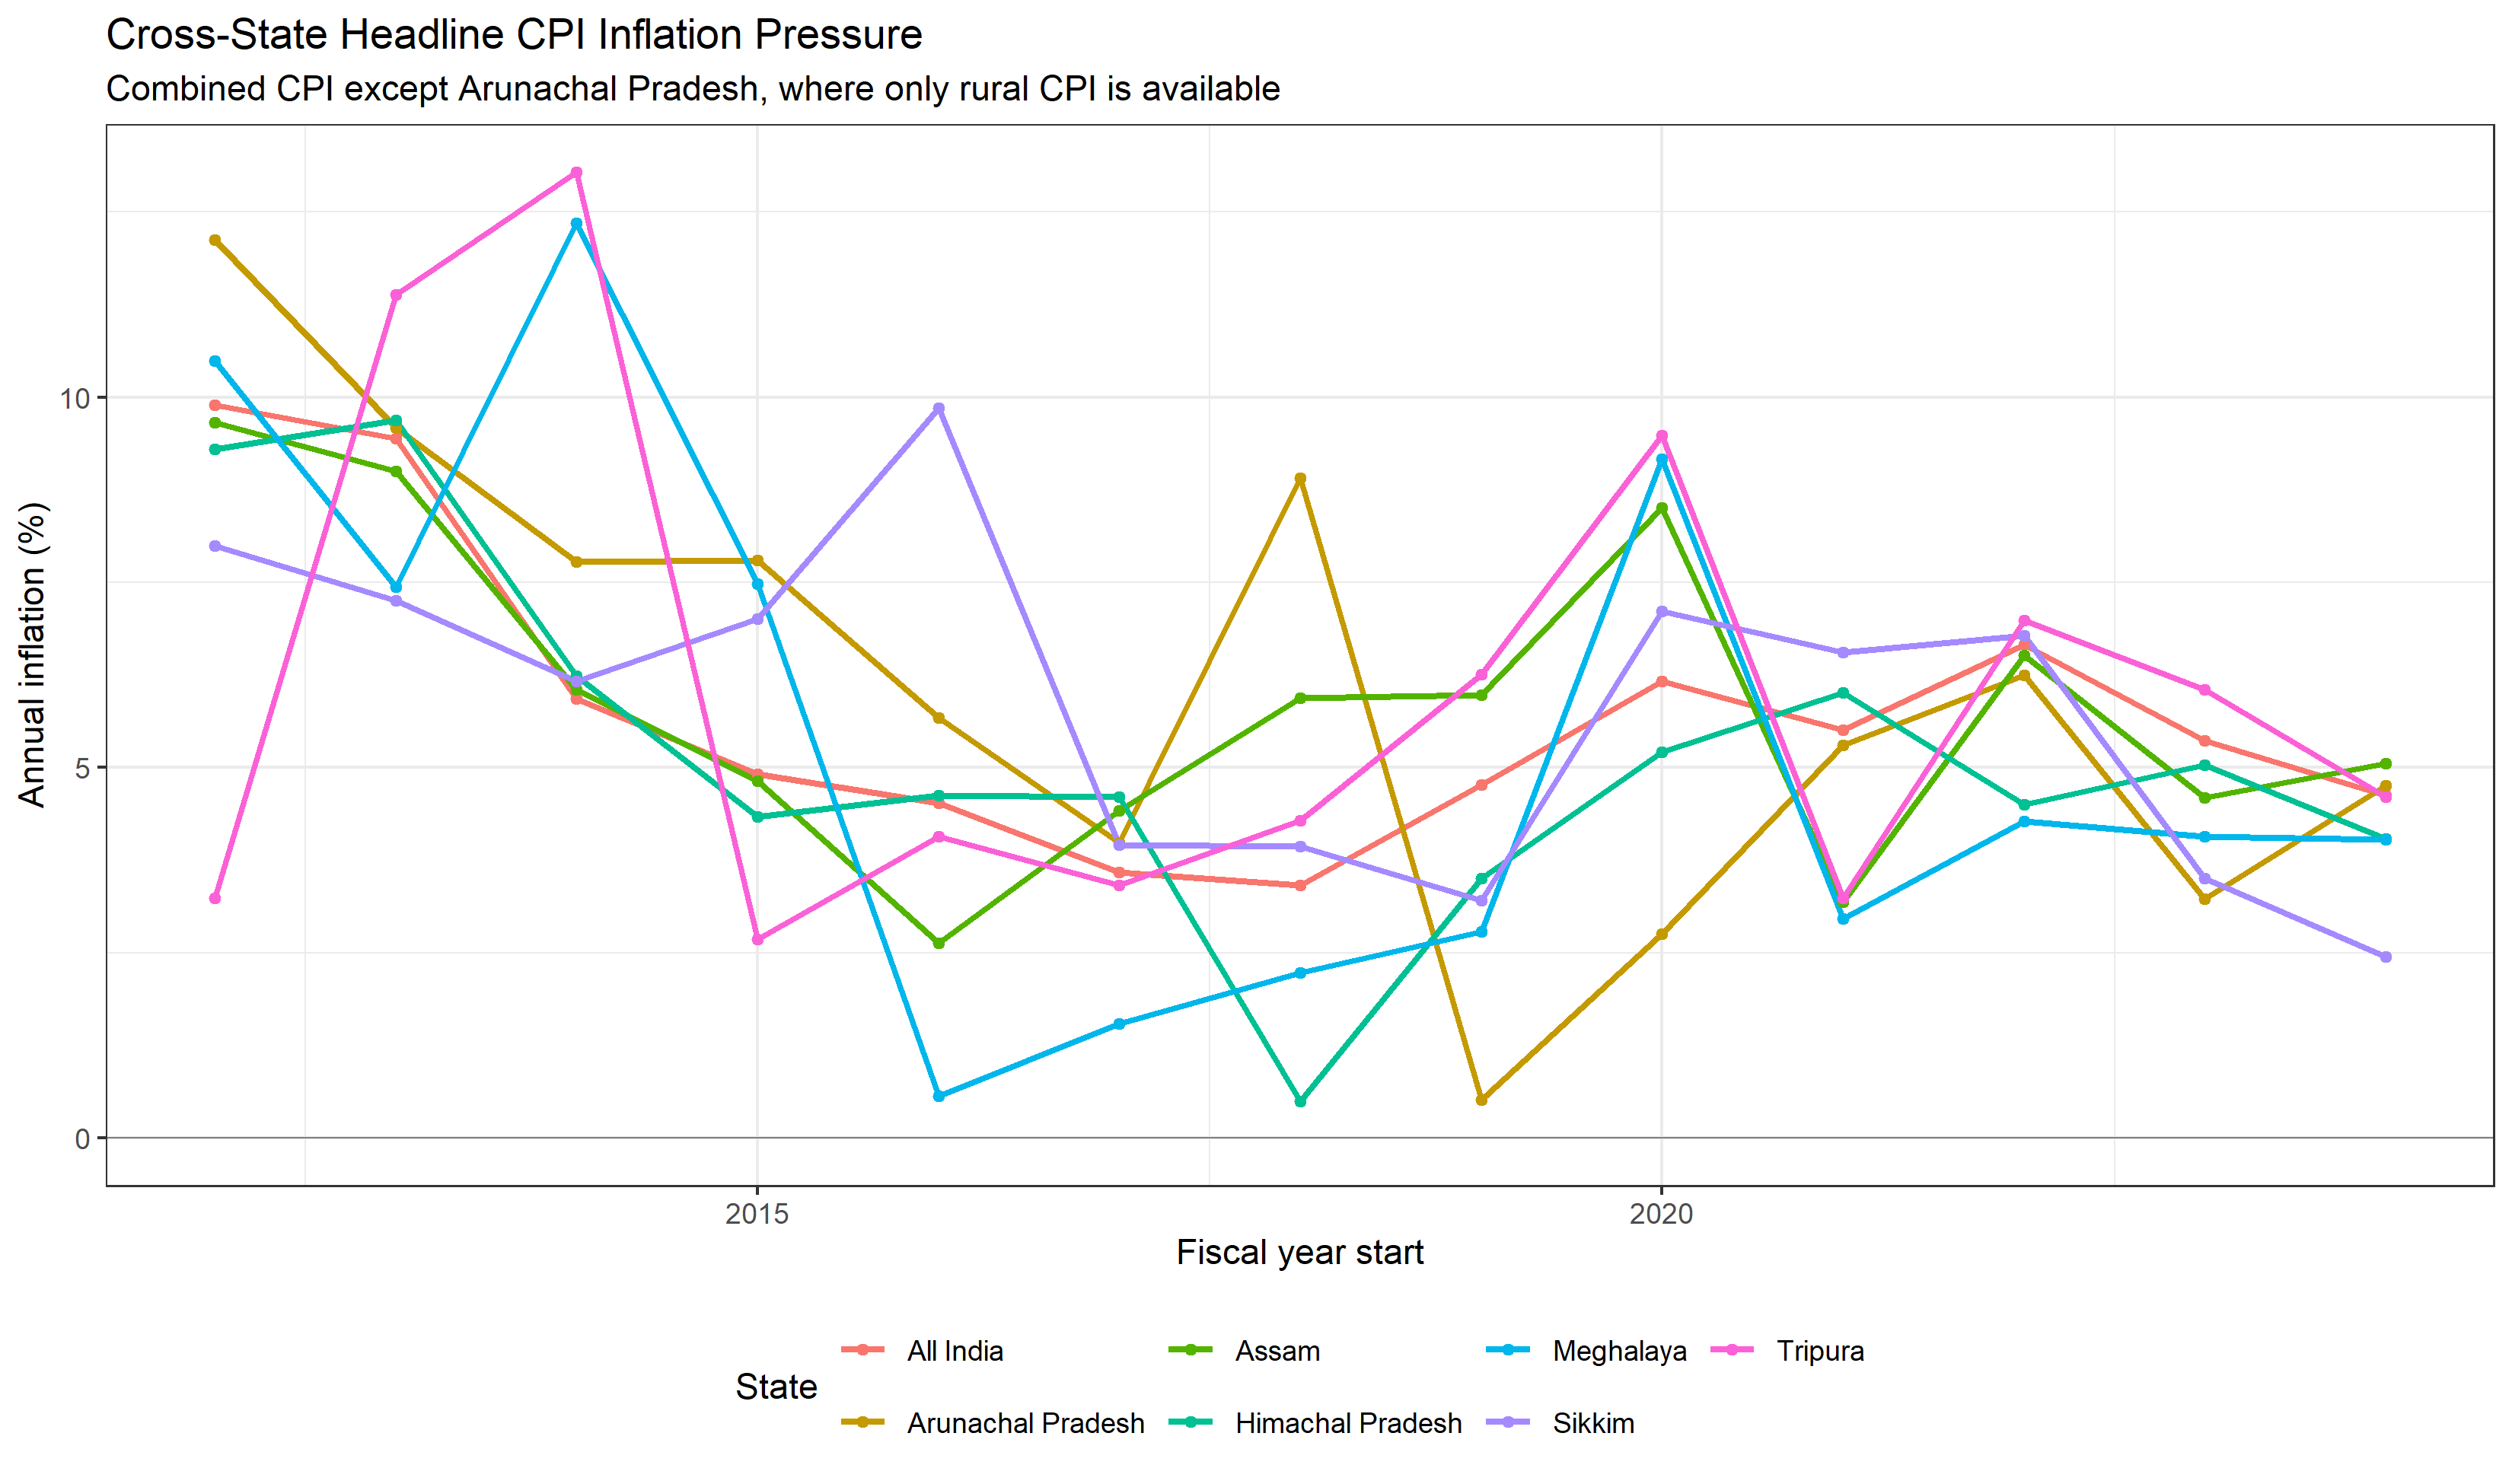
\includegraphics[width=0.92\textwidth]{fig15_cross_state_cpi_pressure.png}
\caption{Cross-state CPI pressure}
\label{fig:cross-state-cpi}
\end{figure}

\begin{figure}[H]
\centering
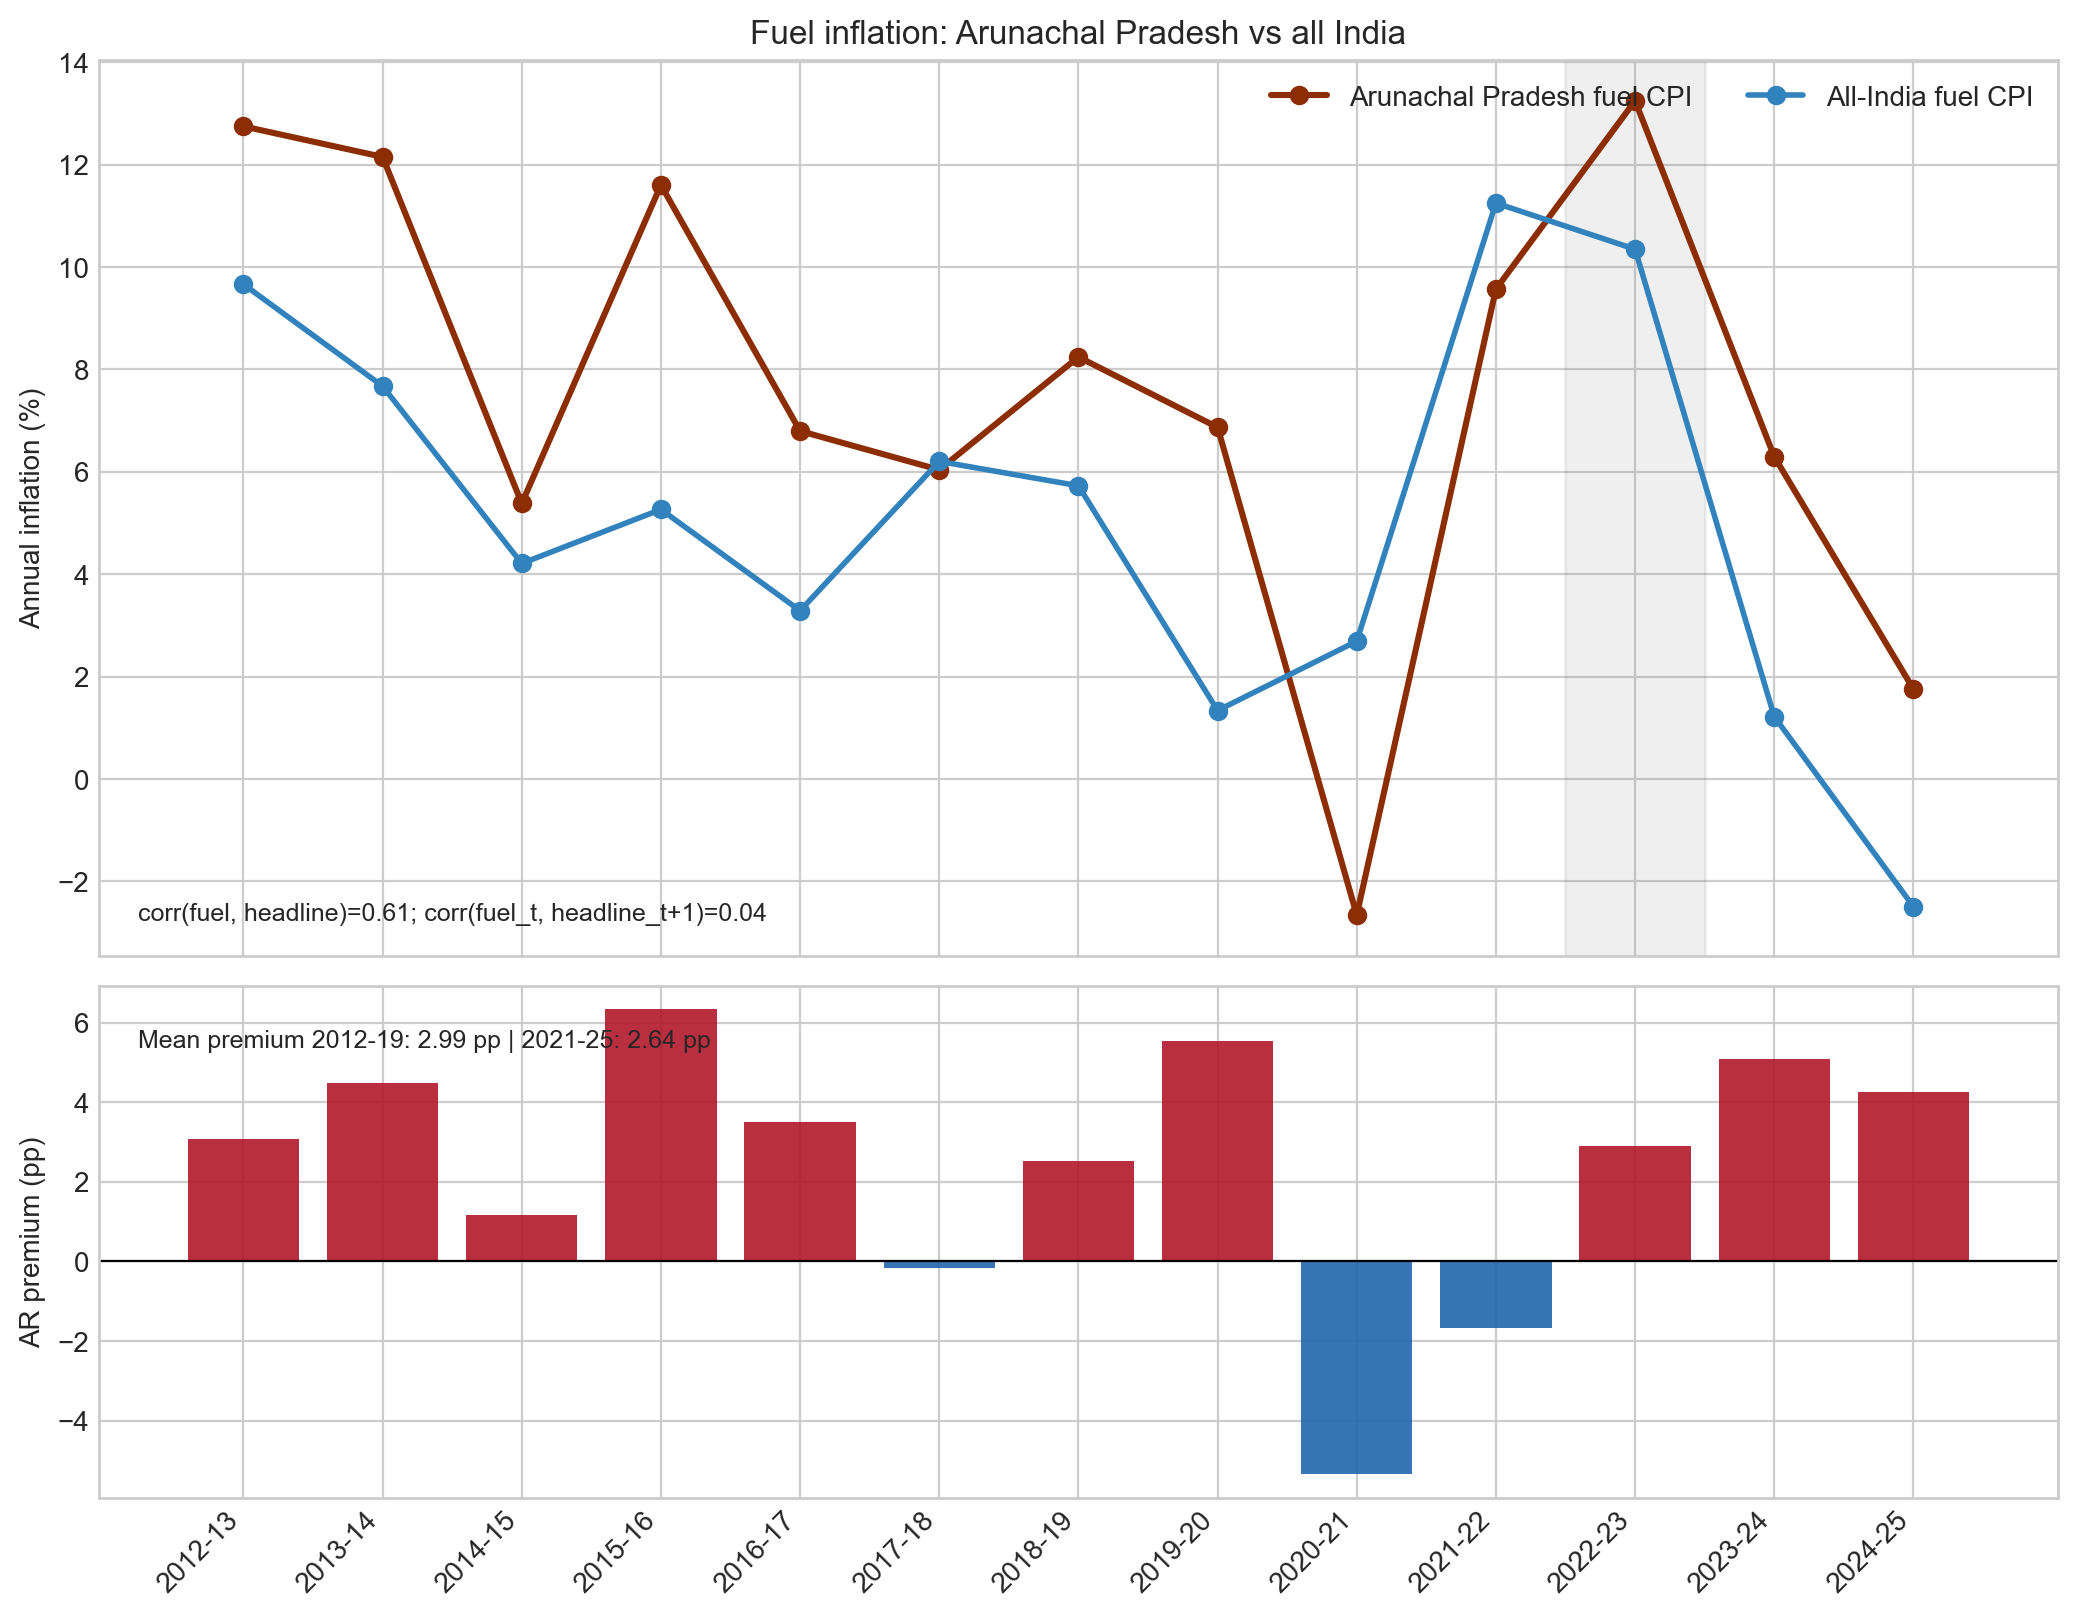
\includegraphics[width=0.92\textwidth]{fig16_fuel_premium_timeseries.png}
\caption{Arunachal Pradesh fuel inflation and the premium over all India}
\label{fig:fuel-premium}
\end{figure}

\FloatBarrier

\section{COVID-19 Shock and Recovery}

The formal COVID-19 pulse dummy for Arunachal Pradesh is negative but not statistically significant at conventional levels: the coefficient is -0.0344 with a robust standard error of 0.0209 and a $p$-value of 0.107. This does not imply that there was no shock. It means that, relative to the fitted trend and the short annual sample, the one-year level shift is imprecisely estimated.

The realised-shock comparison in Table \ref{tab:covid} is more transparent. Arunachal Pradesh's real GSDP fell by 3.69 percent from 2019-20 to 2020-21, compared with a pre-COVID trend CAGR of 5.88 percent. The shock relative to trend is therefore -9.57 percentage points. The fall is milder than Meghalaya's -7.85 percent actual contraction and similar in broad magnitude to Himachal Pradesh and Tripura. The recovery, however, is comparatively weak. Arunachal Pradesh's post-2020 recovery CAGR is 5.02 percent, below Assam, Sikkim, Tripura, and Meghalaya.

That weak rebound fits the composition of the state economy. Recent macro-fiscal evidence shows a structure dominated by services and agriculture, with manufacturing accounting for only 2.2 percent of workers \citep{niti_ncaer_2025_arunachal}. That is not the profile of a state with a large private tradables base ready to snap back after lockdowns. \citet{beyer_francobedoya_galdo_2021} show that COVID-era state heterogeneity in India was partly associated with manufacturing intensity and migration, and they document that Arunachal Pradesh was among the states with an April 2020 electricity decline above 20 percent. In Arunachal Pradesh, transfers and public expenditure can cushion the downturn, but they do not generate the same rebound arithmetic as a broader private-sector base. That helps explain why the initial contraction was not the worst in the sample, yet the subsequent recovery remained slower than in Assam, Tripura, Sikkim, and Meghalaya.

\begin{table}[H]
\centering
\caption{COVID-19 growth shock and recovery}
\label{tab:covid}
\begin{tabular}{L{3.4cm}C{2.3cm}C{2.3cm}C{2.3cm}C{2.3cm}}
\toprule
State & Pre-COVID trend & Actual 2019-20 to 2020-21 & Shock vs trend & Recovery CAGR \\
\midrule
Arunachal Pradesh & 5.88 & -3.69 & -9.57 & 5.02 \\
Assam & 7.82 & 2.95 & -4.86 & 9.00 \\
Sikkim & 8.32 & 0.33 & -7.99 & 8.39 \\
Himachal Pradesh & 6.36 & -4.40 & -10.76 & 5.80 \\
Tripura & 7.14 & -4.36 & -11.50 & 8.40 \\
Meghalaya & 4.35 & -7.85 & -12.20 & 9.54 \\
\bottomrule
\end{tabular}
\begin{flushleft}
\footnotesize Notes: Entries are percent. Recovery CAGR is from 2020-21 to the latest available year, 2024-25 except Sikkim, where the latest available year is 2023-24.
\end{flushleft}
\end{table}

\begin{figure}[H]
\centering
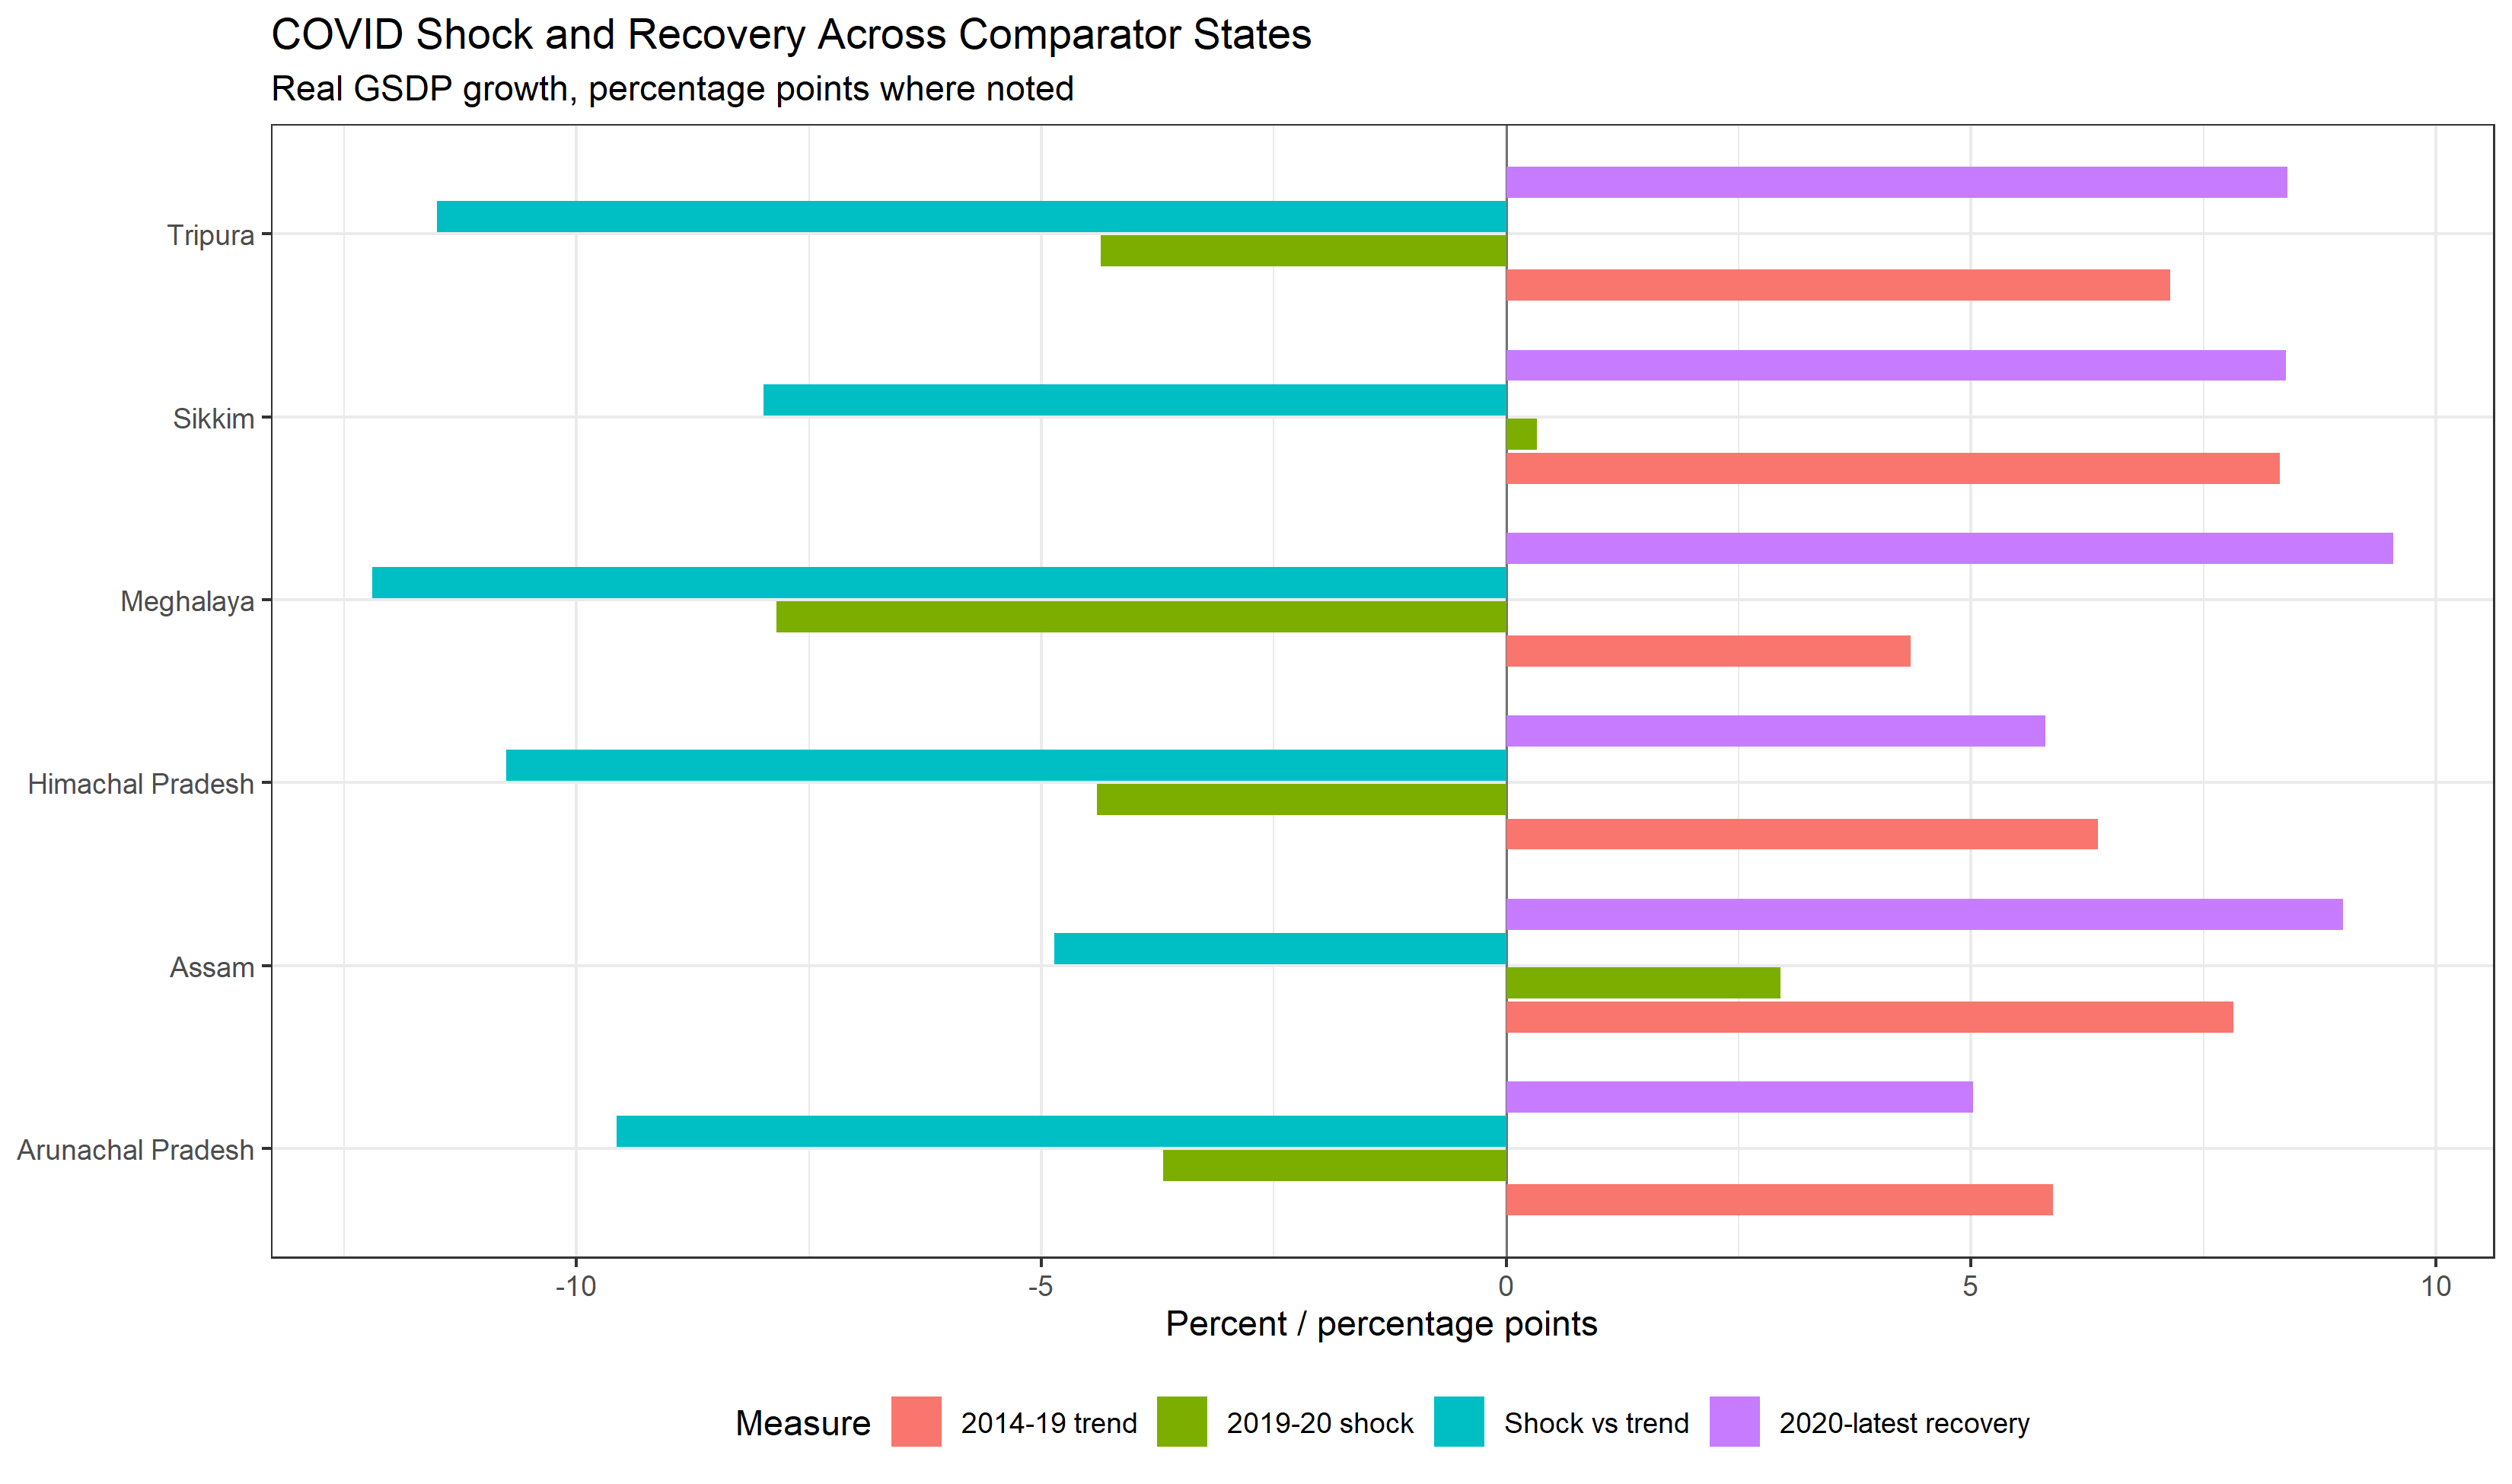
\includegraphics[width=0.92\textwidth]{fig14_covid_shock_and_recovery.png}
\caption{COVID-19 shock and recovery across comparator states}
\label{fig:covid}
\end{figure}

\section{Robustness and Comparator Evidence}

Two robustness exercises support the main interpretation. First, the Arunachal Pradesh break dates are stable to alternative trimming values. With trimming from 0.10 to 0.20, the state continues to show two breaks, dated 1995 and 2013. All-India breaks are more sensitive: the baseline four-break result simplifies to 1978 and 2004 at higher trimming values. This strengthens the caution that India's aggregate growth transition should not be reduced to a single date.

Second, the state-comparator module shows that Arunachal Pradesh is a high-growth state from a low base, but not the strongest post-2003 or post-COVID performer. Figure \ref{fig:real-paths} indexes real GSDP paths, while Figure \ref{fig:liberalisation} compares liberalisation-era growth. Sikkim is the most dramatic small-state high-growth benchmark after 2003. Assam is weaker before 2013 but outperforms Arunachal Pradesh after 2013. Tripura's 1991-2003 and 2003-13 performance is stronger than Arunachal Pradesh's. Appendix Figure \ref{fig:sigma} is consistent with the broader divergence literature: cross-state dispersion in log per-capita NSDP does not show a clean monotonic decline, which is exactly why unconditional catch-up is the wrong prior for a frontier state \citep{sachs_bajpai_ramiah_2002,bhattacharya_sakthivel_2004,bandyopadhyay_2011}. These comparisons sharpen the paper's thesis: Arunachal Pradesh's growth is impressive in levels and early growth rates, but it is not a uniquely successful post-reform growth acceleration.

\begin{figure}[H]
\centering
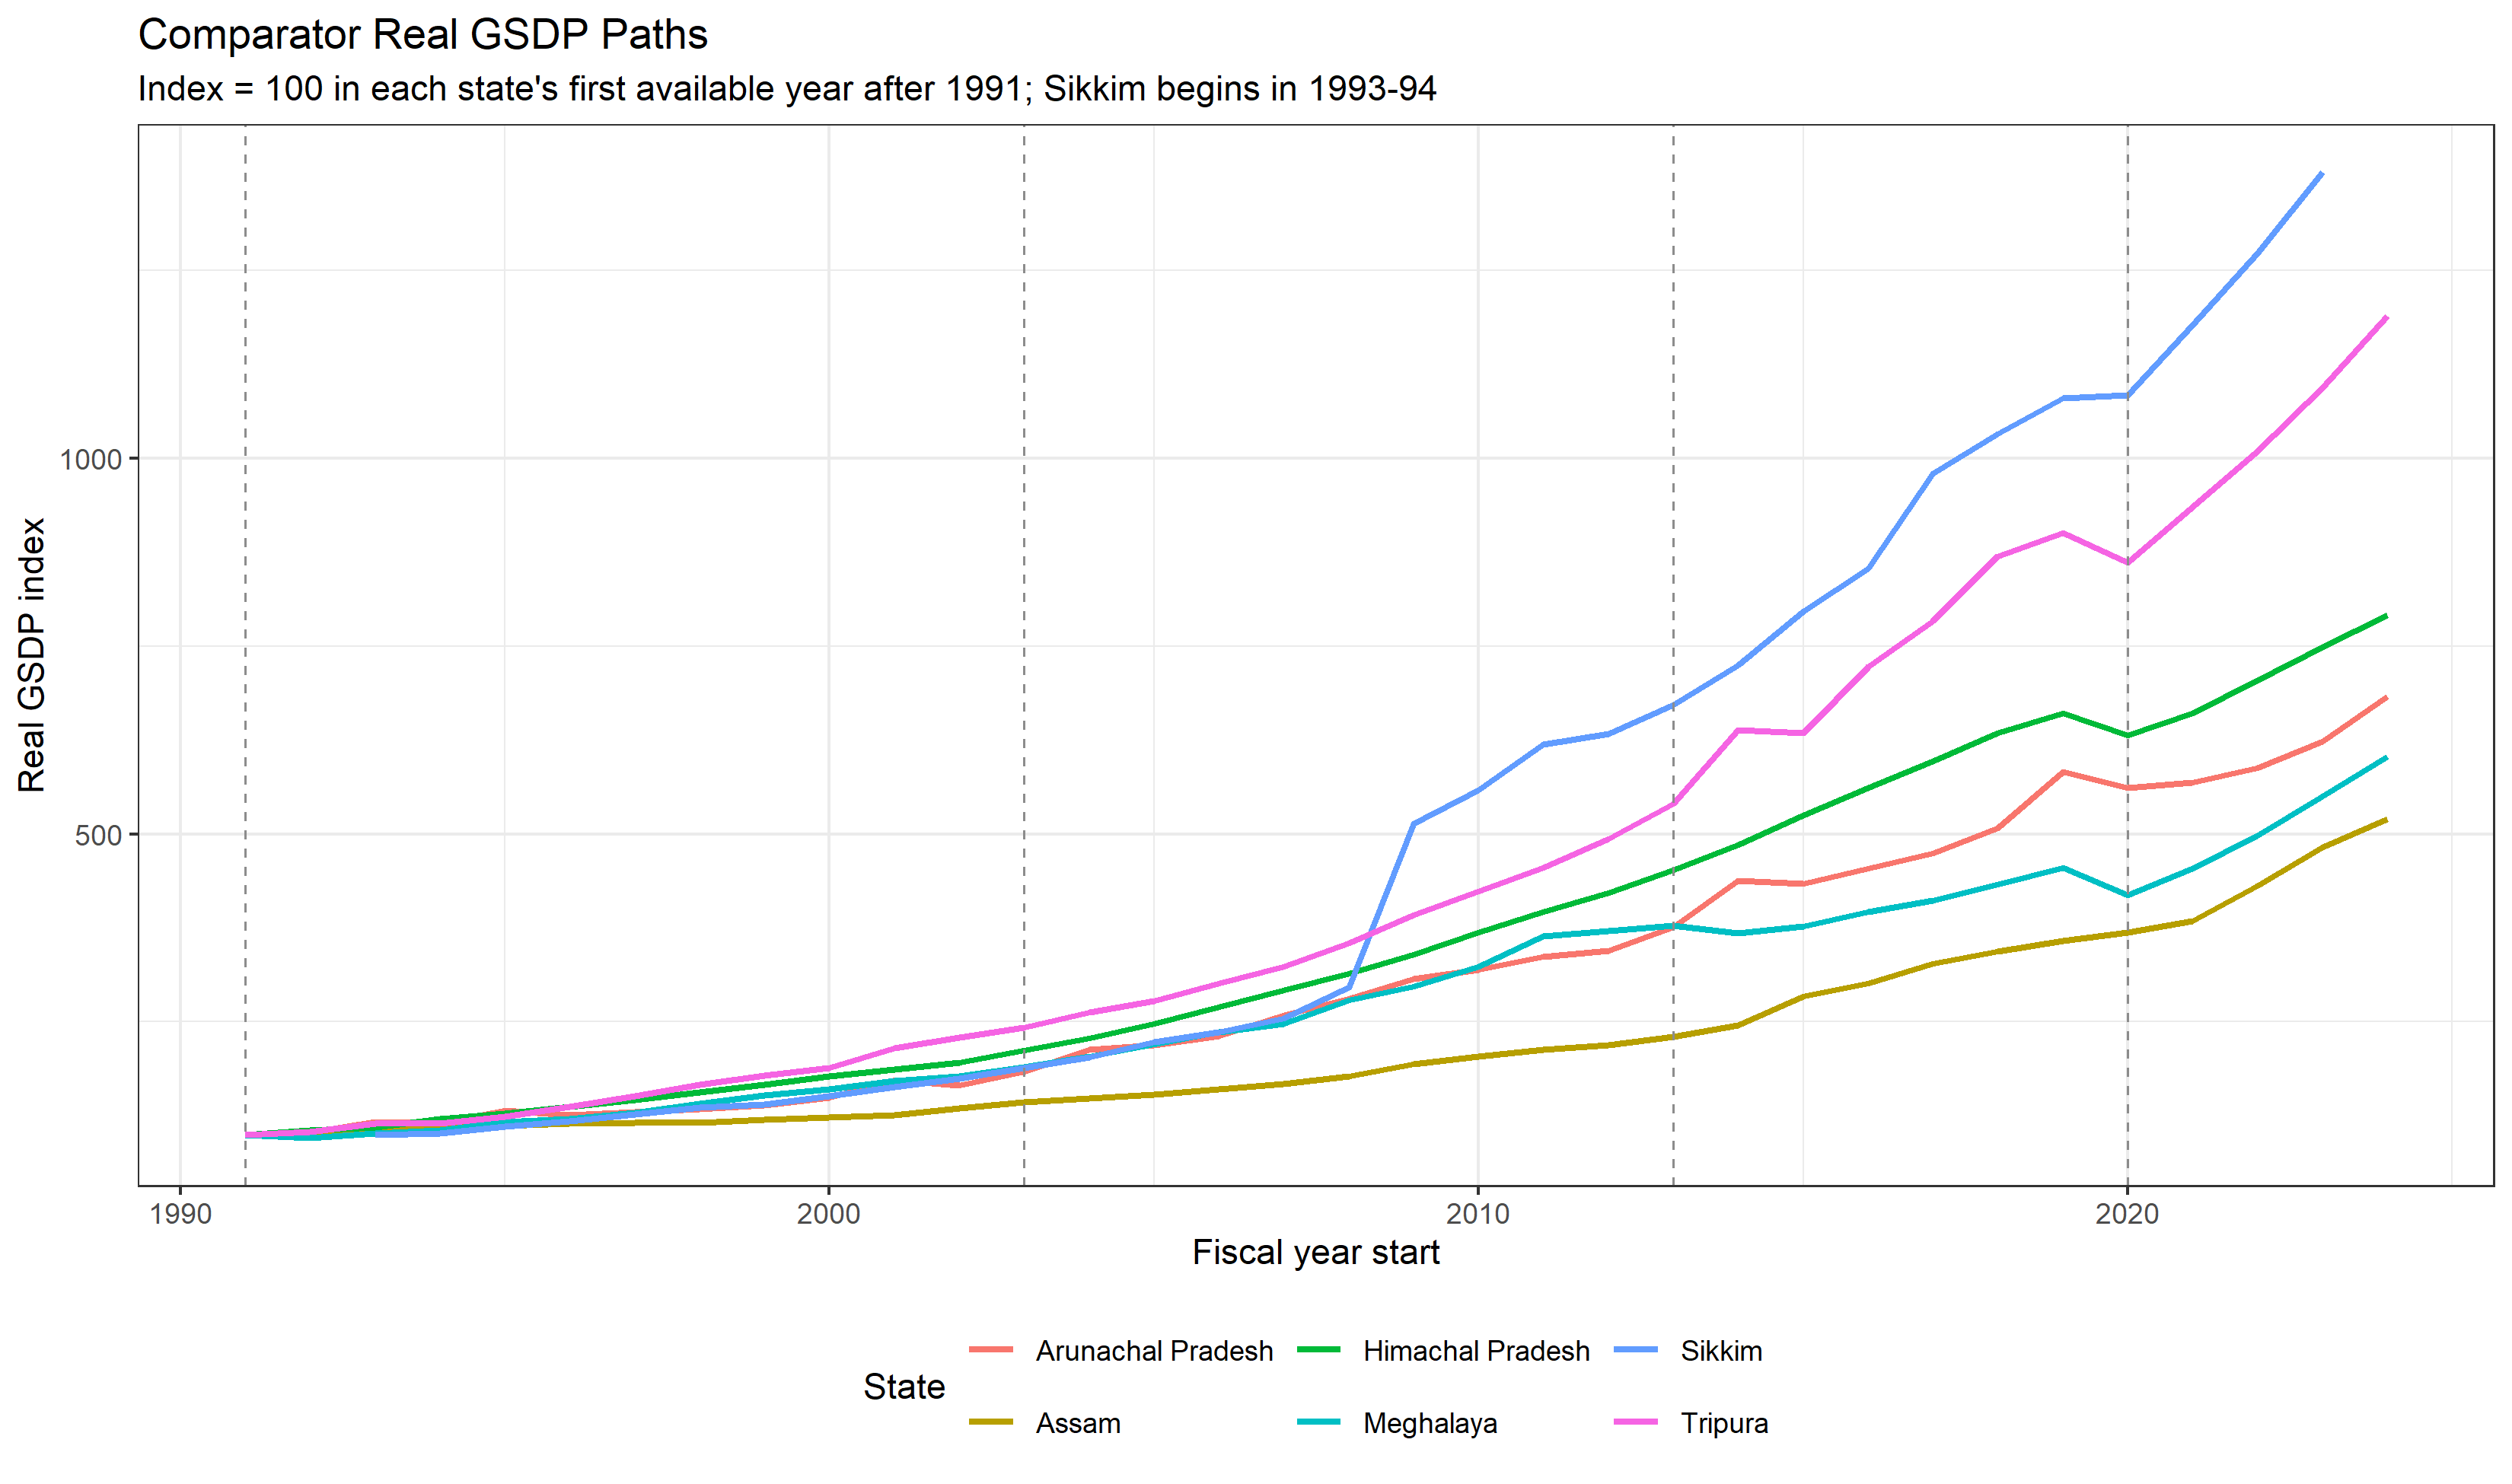
\includegraphics[width=0.92\textwidth]{fig12_comparator_real_growth_paths.png}
\caption{Indexed real GSDP paths across comparator states}
\label{fig:real-paths}
\end{figure}

\begin{figure}[H]
\centering
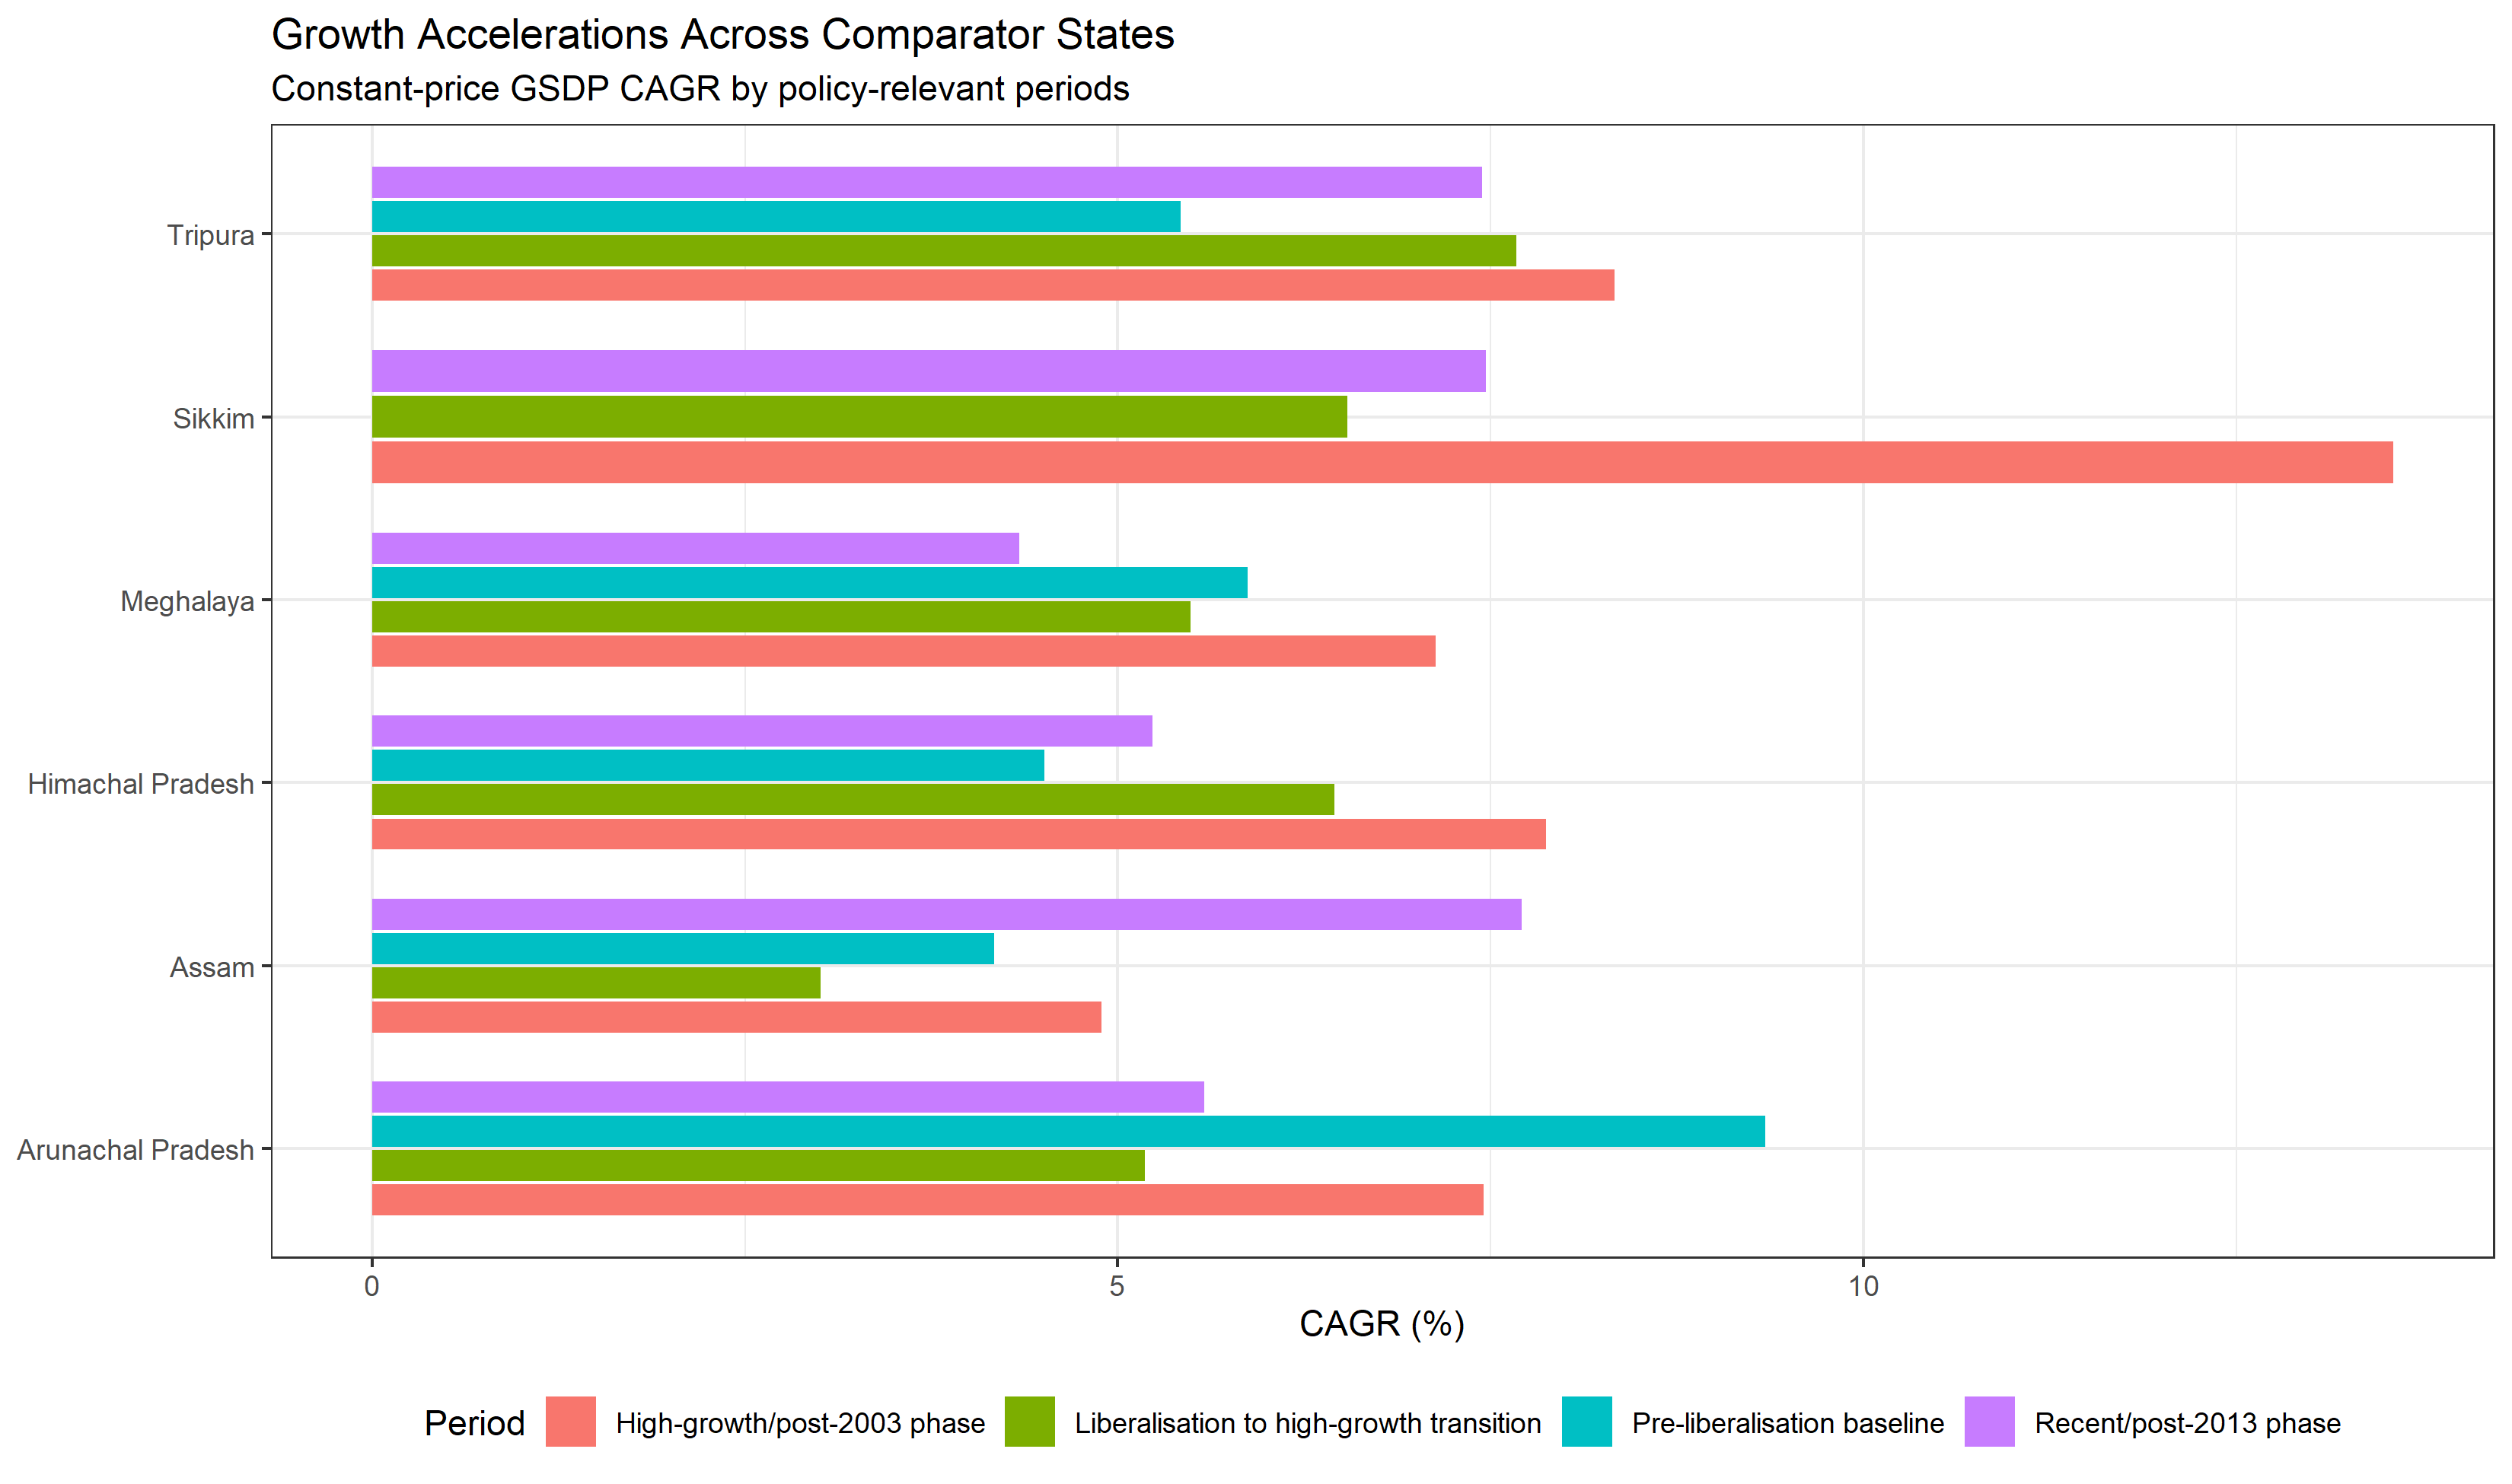
\includegraphics[width=0.92\textwidth]{fig13_liberalisation_growth_comparison.png}
\caption{Growth comparison around liberalisation and later regimes}
\label{fig:liberalisation}
\end{figure}

\section{Discussion}

The results suggest three substantive conclusions. First, Arunachal Pradesh's growth history is not well described by the standard all-India liberalisation narrative. The state does not show a 1991 break, and its pre-1991 growth rate is higher than its 1991-2003 growth rate. This is consistent with the literature arguing that India's growth transition itself is more complex than a single reform date, and it is even more relevant for a frontier state whose economic base differs sharply from the national average.

Second, growth has not produced deep structural transformation. The sectoral shift away from agriculture is real, but the receiving sector is mainly services. In Arunachal Pradesh this likely reflects public administration, construction-linked activity, and transfer-financed services more than autonomous private-sector dynamism. The fiscal evidence should therefore be read as corroboration, not as decoration. Appendix Figure \ref{fig:fiscal-dependence} shows a fiscal dependence ratio averaging 87.4 percent, while Appendix Figure \ref{fig:own-revenue} shows that own revenue remains modest relative to revenue expenditure. Combined with the services-heavy output structure and the very small manufacturing employment share, those fiscal patterns make the transfer-dependent label descriptive rather than rhetorical \citep{govil_chauhan_2024,niti_ncaer_2025_arunachal}. The main causal evidence in this paper still comes from break timing, sectoral composition, and inflation behavior rather than from fiscal ratios alone.

Third, inflation behaves like a partially integrated frontier-market phenomenon. Arunachal Pradesh does not move independently of all India: quarterly headline CPI inflation has a positive correlation of 0.54 with the national series. But the relationship is far from one-for-one, volatility is higher, and fuel inflation is especially elevated. This is exactly where terrain and logistics should matter. The CPI evidence also warns against over-precision. The absence of urban CPI, the missing 2020 months, and the narrow state core-inflation measure all limit comparability. Even so, the broad result is robust: Arunachal Pradesh faces more volatile consumer-price pressure than all India, and its inflation experience must be read through food, fuel, and transport-cost channels.

\section{Conclusion}

This paper provides a complete empirical assessment of Arunachal Pradesh's growth and inflation performance under the assignment brief. The evidence shows a state that grew rapidly but did not experience a standard post-1991 acceleration. Its structural breaks are dated at 1995-96 and 2013-14; its trend growth declines across regimes; and its pre-liberalisation growth exceeds its 1991-2003 growth. Inflation is slightly higher on average and clearly more volatile than all India, with a marked fuel component whose premium persists even after the pandemic. The COVID-19 output shock was real but not the most severe among comparable hill and Northeast states, while the recovery has been weaker than several comparators.

The best interpretation is therefore not simply that Arunachal Pradesh is a high-growth state. It is that Arunachal Pradesh is a transfer-dependent frontier economy: public expenditure and central transfers sustain demand and services-led output expansion, while terrain, thin markets, and limited industrial transformation shape inflation and long-run growth constraints. The policy implication is that macroeconomic performance should be judged not only by the level of GSDP growth, but also by the source, composition, volatility, and resilience of that growth.

\newpage
\appendix

\section{Additional Tables}

\begin{longtable}{L{2.2cm}C{2.2cm}C{2.2cm}C{2.2cm}C{2.2cm}}
\caption{Annual headline and core inflation}
\label{tab:annual-inflation}\\
\toprule
Fiscal year & AR headline & AR core & India headline & India core \\
\midrule
\endfirsthead
\toprule
Fiscal year & AR headline & AR core & India headline & India core \\
\midrule
\endhead
2011-12 & n.a. & n.a. & n.a. & n.a. \\
2012-13 & 12.12 & 9.95 & 10.05 & 8.96 \\
2013-14 & 9.59 & 8.66 & 9.38 & 7.03 \\
2014-15 & 7.78 & 5.76 & 5.83 & 5.26 \\
2015-16 & 7.80 & 7.86 & 4.91 & 4.34 \\
2016-17 & 5.67 & 6.37 & 4.52 & 4.72 \\
2017-18 & 3.99 & 4.78 & 3.59 & 4.54 \\
2018-19 & 8.91 & 8.09 & 3.41 & 5.78 \\
2019-20 & 0.54 & 4.01 & 4.77 & 4.02 \\
2020-21 & 3.23 & 0.11 & 6.16 & 5.31 \\
2021-22 & 4.79 & 5.34 & 5.51 & 6.09 \\
2022-23 & 6.24 & 5.42 & 6.65 & 6.30 \\
2023-24 & 3.22 & 4.13 & 5.36 & 4.38 \\
2024-25 & 4.76 & 3.88 & 4.63 & 3.60 \\
\bottomrule
\end{longtable}

\begin{table}[H]
\centering
\caption{Inflation before and after COVID-19}
\label{tab:inflation-subperiods}
\begin{tabular}{L{4cm}C{2cm}C{2cm}C{2cm}C{2cm}C{1.4cm}}
\toprule
Period & AR mean & AR SD & India mean & India SD & N \\
\midrule
Pre-COVID, 2012-2019 & 7.10 & 3.65 & 5.87 & 2.61 & 33 \\
COVID and post-COVID, 2020 onward & 4.18 & 1.82 & 5.15 & 1.66 & 23 \\
\bottomrule
\end{tabular}
\end{table}

\begin{table}[H]
\centering
\caption{Inflation comparability and co-movement diagnostics}
\label{tab:inflation-diagnostics}
\begin{tabular}{L{8.2cm}C{2.0cm}L{3.8cm}}
\toprule
Diagnostic & Value & Note \\
\midrule
Housing weight in the population-weighted combined national core basket & 22.01 & percent of combined core basket \\
Housing weight in the population-weighted combined national core basket & 9.83 & weight points \\
Mean absolute change in annual all-India core inflation when housing is excluded, 2012-13 to 2024-25 & 0.29 & percentage points \\
Maximum absolute change in annual all-India core inflation when housing is excluded & 0.71 & percentage points, in 2021-22 \\
Pearson correlation: quarterly Arunachal Pradesh vs all-India headline inflation, full overlap & 0.54 & $p<0.001$, $N=56$ \\
Pearson correlation: quarterly Arunachal Pradesh vs all-India headline inflation, pre-COVID & 0.70 & $p<0.001$, $N=29$ \\
Pearson correlation: quarterly Arunachal Pradesh vs all-India headline inflation, 2020 onward & 0.24 & $p=0.221$, $N=27$ \\
\bottomrule
\end{tabular}
\end{table}

\begin{table}[H]
\centering
\caption{Break-date trimming sensitivity}
\label{tab:trimming}
\begin{tabular}{C{1.8cm}C{2.5cm}L{4cm}C{2.5cm}L{3cm}}
\toprule
Trimming & India breaks & India break years & AR breaks & AR break years \\
\midrule
0.10 & 4 & 1971, 1978, 2003, 2018 & 2 & 1995, 2013 \\
0.12 & 2 & 1978, 2004 & 2 & 1995, 2013 \\
0.15 & 2 & 1978, 2004 & 2 & 1995, 2013 \\
0.18 & 2 & 1978, 2004 & 2 & 1995, 2013 \\
0.20 & 2 & 1978, 2004 & 2 & 1995, 2013 \\
\bottomrule
\end{tabular}
\end{table}

\begin{landscape}
\scriptsize
\setlength{\tabcolsep}{3pt}
\begin{longtable}{L{2.8cm}L{3.2cm}C{1.15cm}C{1.15cm}C{1.15cm}C{1.15cm}C{1.15cm}C{1.15cm}L{3.6cm}}
\caption{Comparator data coverage audit}
\label{tab:coverage-audit}\\
\toprule
State & Role & GSDP first & GSDP last & GSDP miss. & PC first & PC last & CPI miss. & CPI sector and caveat \\
\midrule
\endfirsthead
\toprule
State & Role & GSDP first & GSDP last & GSDP miss. & PC first & PC last & CPI miss. & CPI sector and caveat \\
\midrule
\endhead
Arunachal Pradesh & Assigned frontier state & 1980 & 2024 & 0 & 1970 & 2024 & 2 & Rural; exact cross-state core not computed \\
Assam & Northeast regional baseline & 1980 & 2024 & 0 & 1970 & 2024 & 2 & Combined; exact cross-state core not computed \\
Himachal Pradesh & Hill-state counterfactual & 1980 & 2024 & 0 & 1967 & 2024 & 2 & Combined; exact cross-state core not computed \\
Manipur & Data-audit NE comparator & 1980 & 2023 & 1 & 1960 & 2023 & 3 & Combined; exact cross-state core not computed \\
Meghalaya & Northeast robustness comparator & 1980 & 2024 & 0 & 1980 & 2024 & 2 & Combined; exact cross-state core not computed \\
Mizoram & Data-audit NE comparator & 1999 & 2023 & 9 & 1999 & 2023 & 2 & Combined; exact cross-state core not computed \\
Nagaland & Data-audit NE comparator & 1993 & 2023 & 3 & 1980 & 2023 & 3 & Combined; exact cross-state core not computed \\
Sikkim & Small Himalayan benchmark & 1993 & 2023 & 3 & 1993 & 2023 & 2 & Combined; exact cross-state core not computed \\
Tripura & Northeast robustness comparator & 1980 & 2024 & 0 & 1960 & 2024 & 2 & Combined; exact cross-state core not computed \\
Uttarakhand & Hill-state robustness comparator & 1980 & 2024 & 0 & 1993 & 2024 & 2 & Combined; exact cross-state core not computed \\
\bottomrule
\end{longtable}
\setlength{\tabcolsep}{6pt}
\end{landscape}

\begin{table}[H]
\centering
\caption{Recent Arunachal Pradesh fiscal indicators}
\label{tab:fiscal-bridge}
\small
\begin{tabular}{L{2cm}C{1.8cm}C{2.1cm}C{2.1cm}C{2.1cm}C{2.1cm}}
\toprule
Fiscal year & Figure type & Rev. bal./GSDP & Fiscal bal./GSDP & Primary bal./GSDP & Interest/Rev. exp. \\
\midrule
2021-22 & Account & 16.47 & 3.25 & 5.63 & 4.91 \\
2022-23 & Account & 17.84 & -0.79 & 1.55 & 4.79 \\
2023-24 & Account & 17.83 & 8.06 & 10.29 & 4.17 \\
2024-25 & Revised & 16.30 & 2.90 & 5.04 & 3.60 \\
2025-26 & Budget & 9.44 & 2.61 & 4.66 & 3.32 \\
\bottomrule
\end{tabular}
\begin{flushleft}
\footnotesize Notes: This table is included as supporting fiscal context for the transfer-dependent growth interpretation. Positive fiscal balance denotes surplus.
\end{flushleft}
\end{table}

\section{Additional Figures}

\begin{figure}[H]
\centering
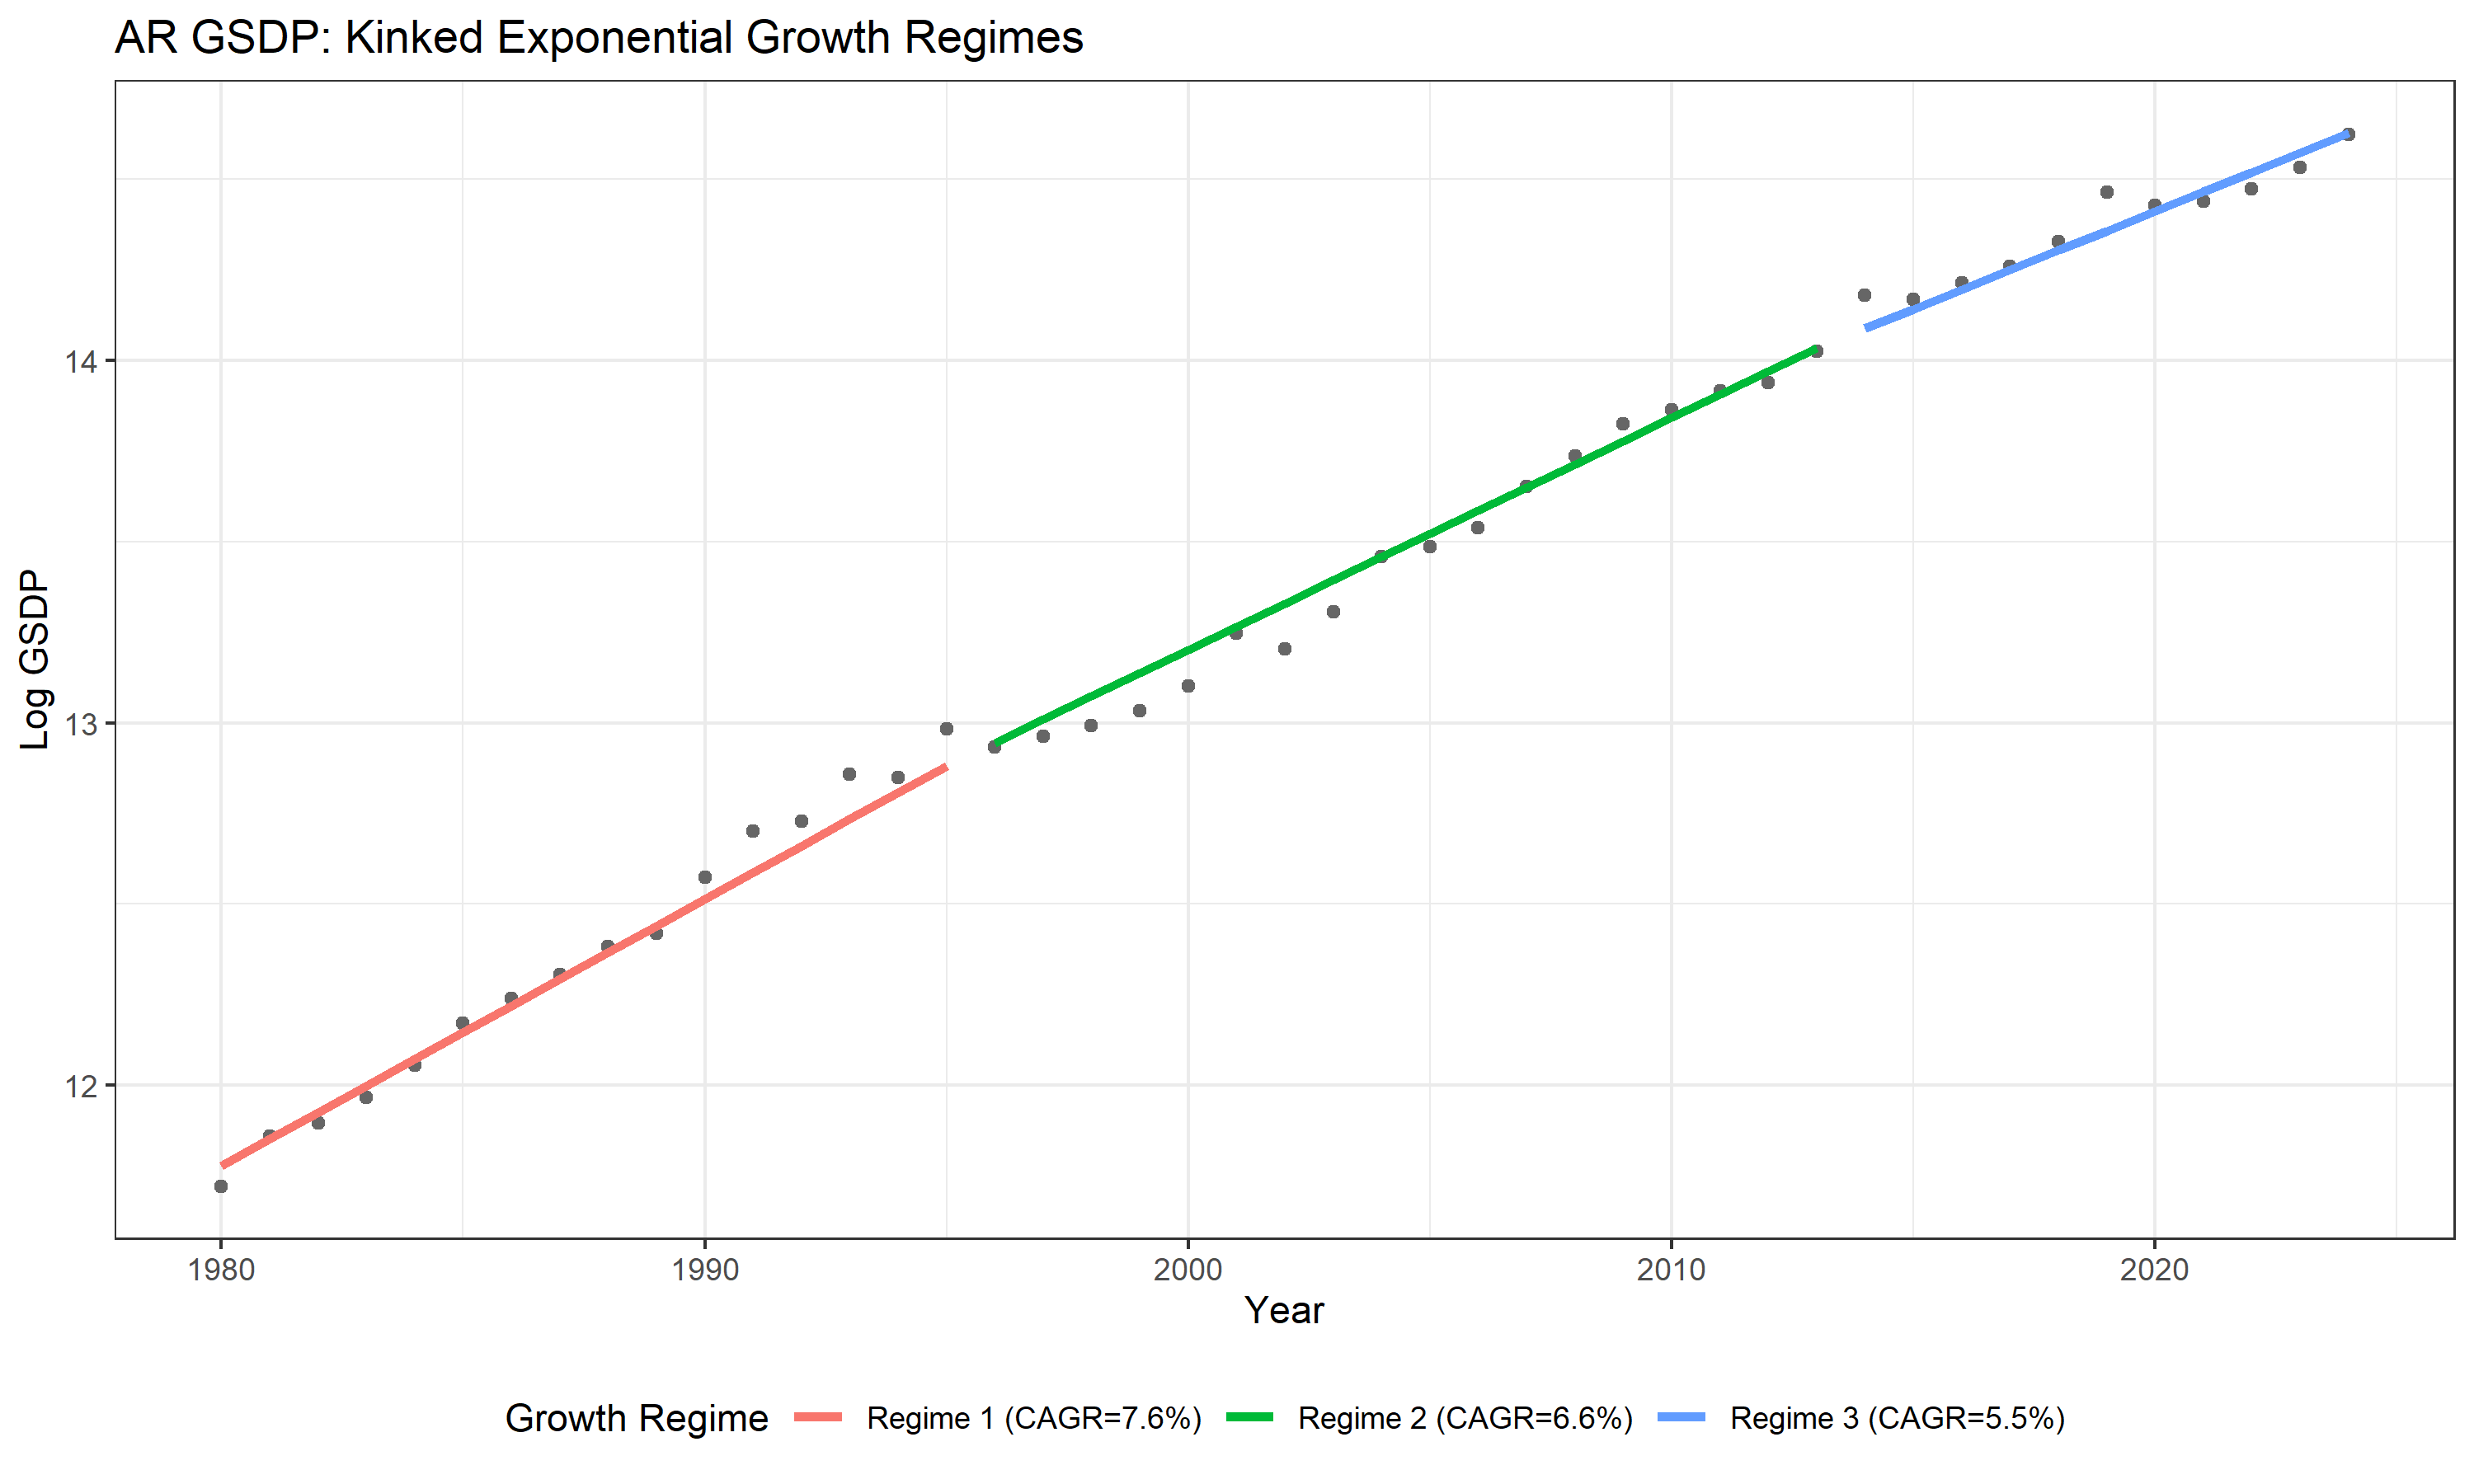
\includegraphics[width=0.92\textwidth]{fig4_ar_kinked_fit.png}
\caption{Kinked exponential fit for Arunachal Pradesh}
\label{fig:ar-kinked}
\end{figure}

\begin{figure}[H]
\centering
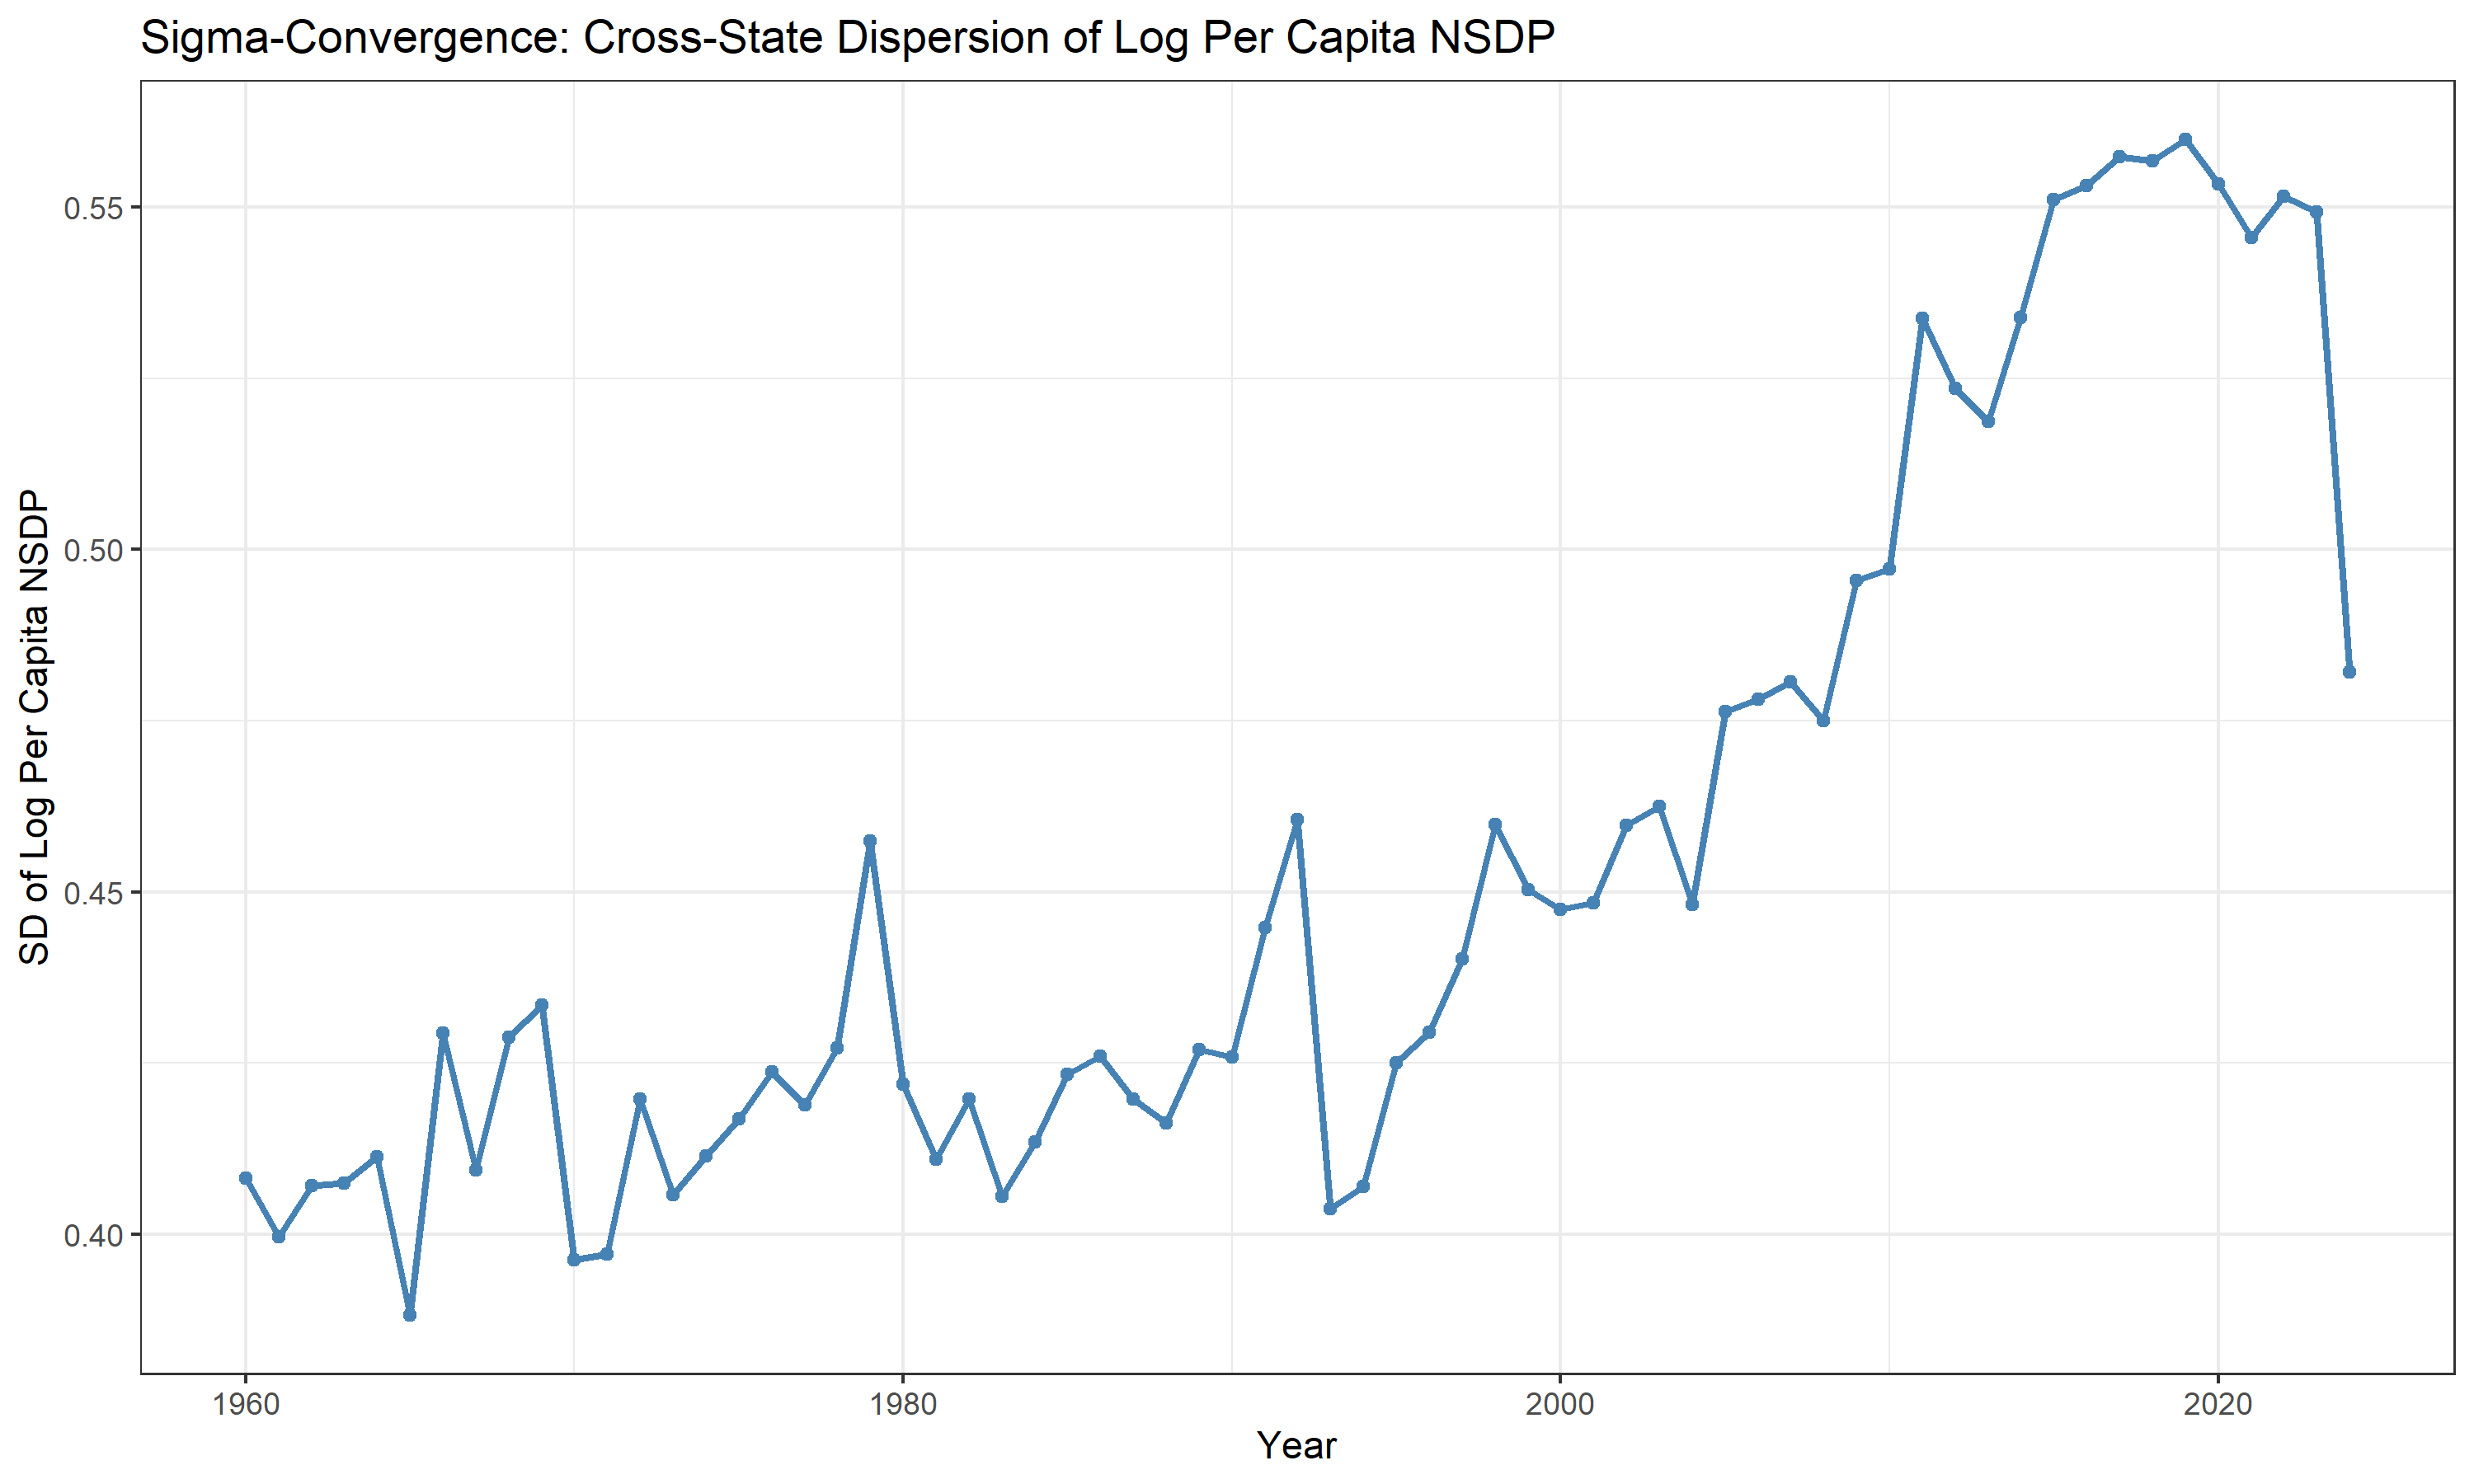
\includegraphics[width=0.92\textwidth]{fig7_sigma_convergence.png}
\caption{Sigma convergence across Indian states}
\label{fig:sigma}
\end{figure}

\begin{figure}[H]
\centering
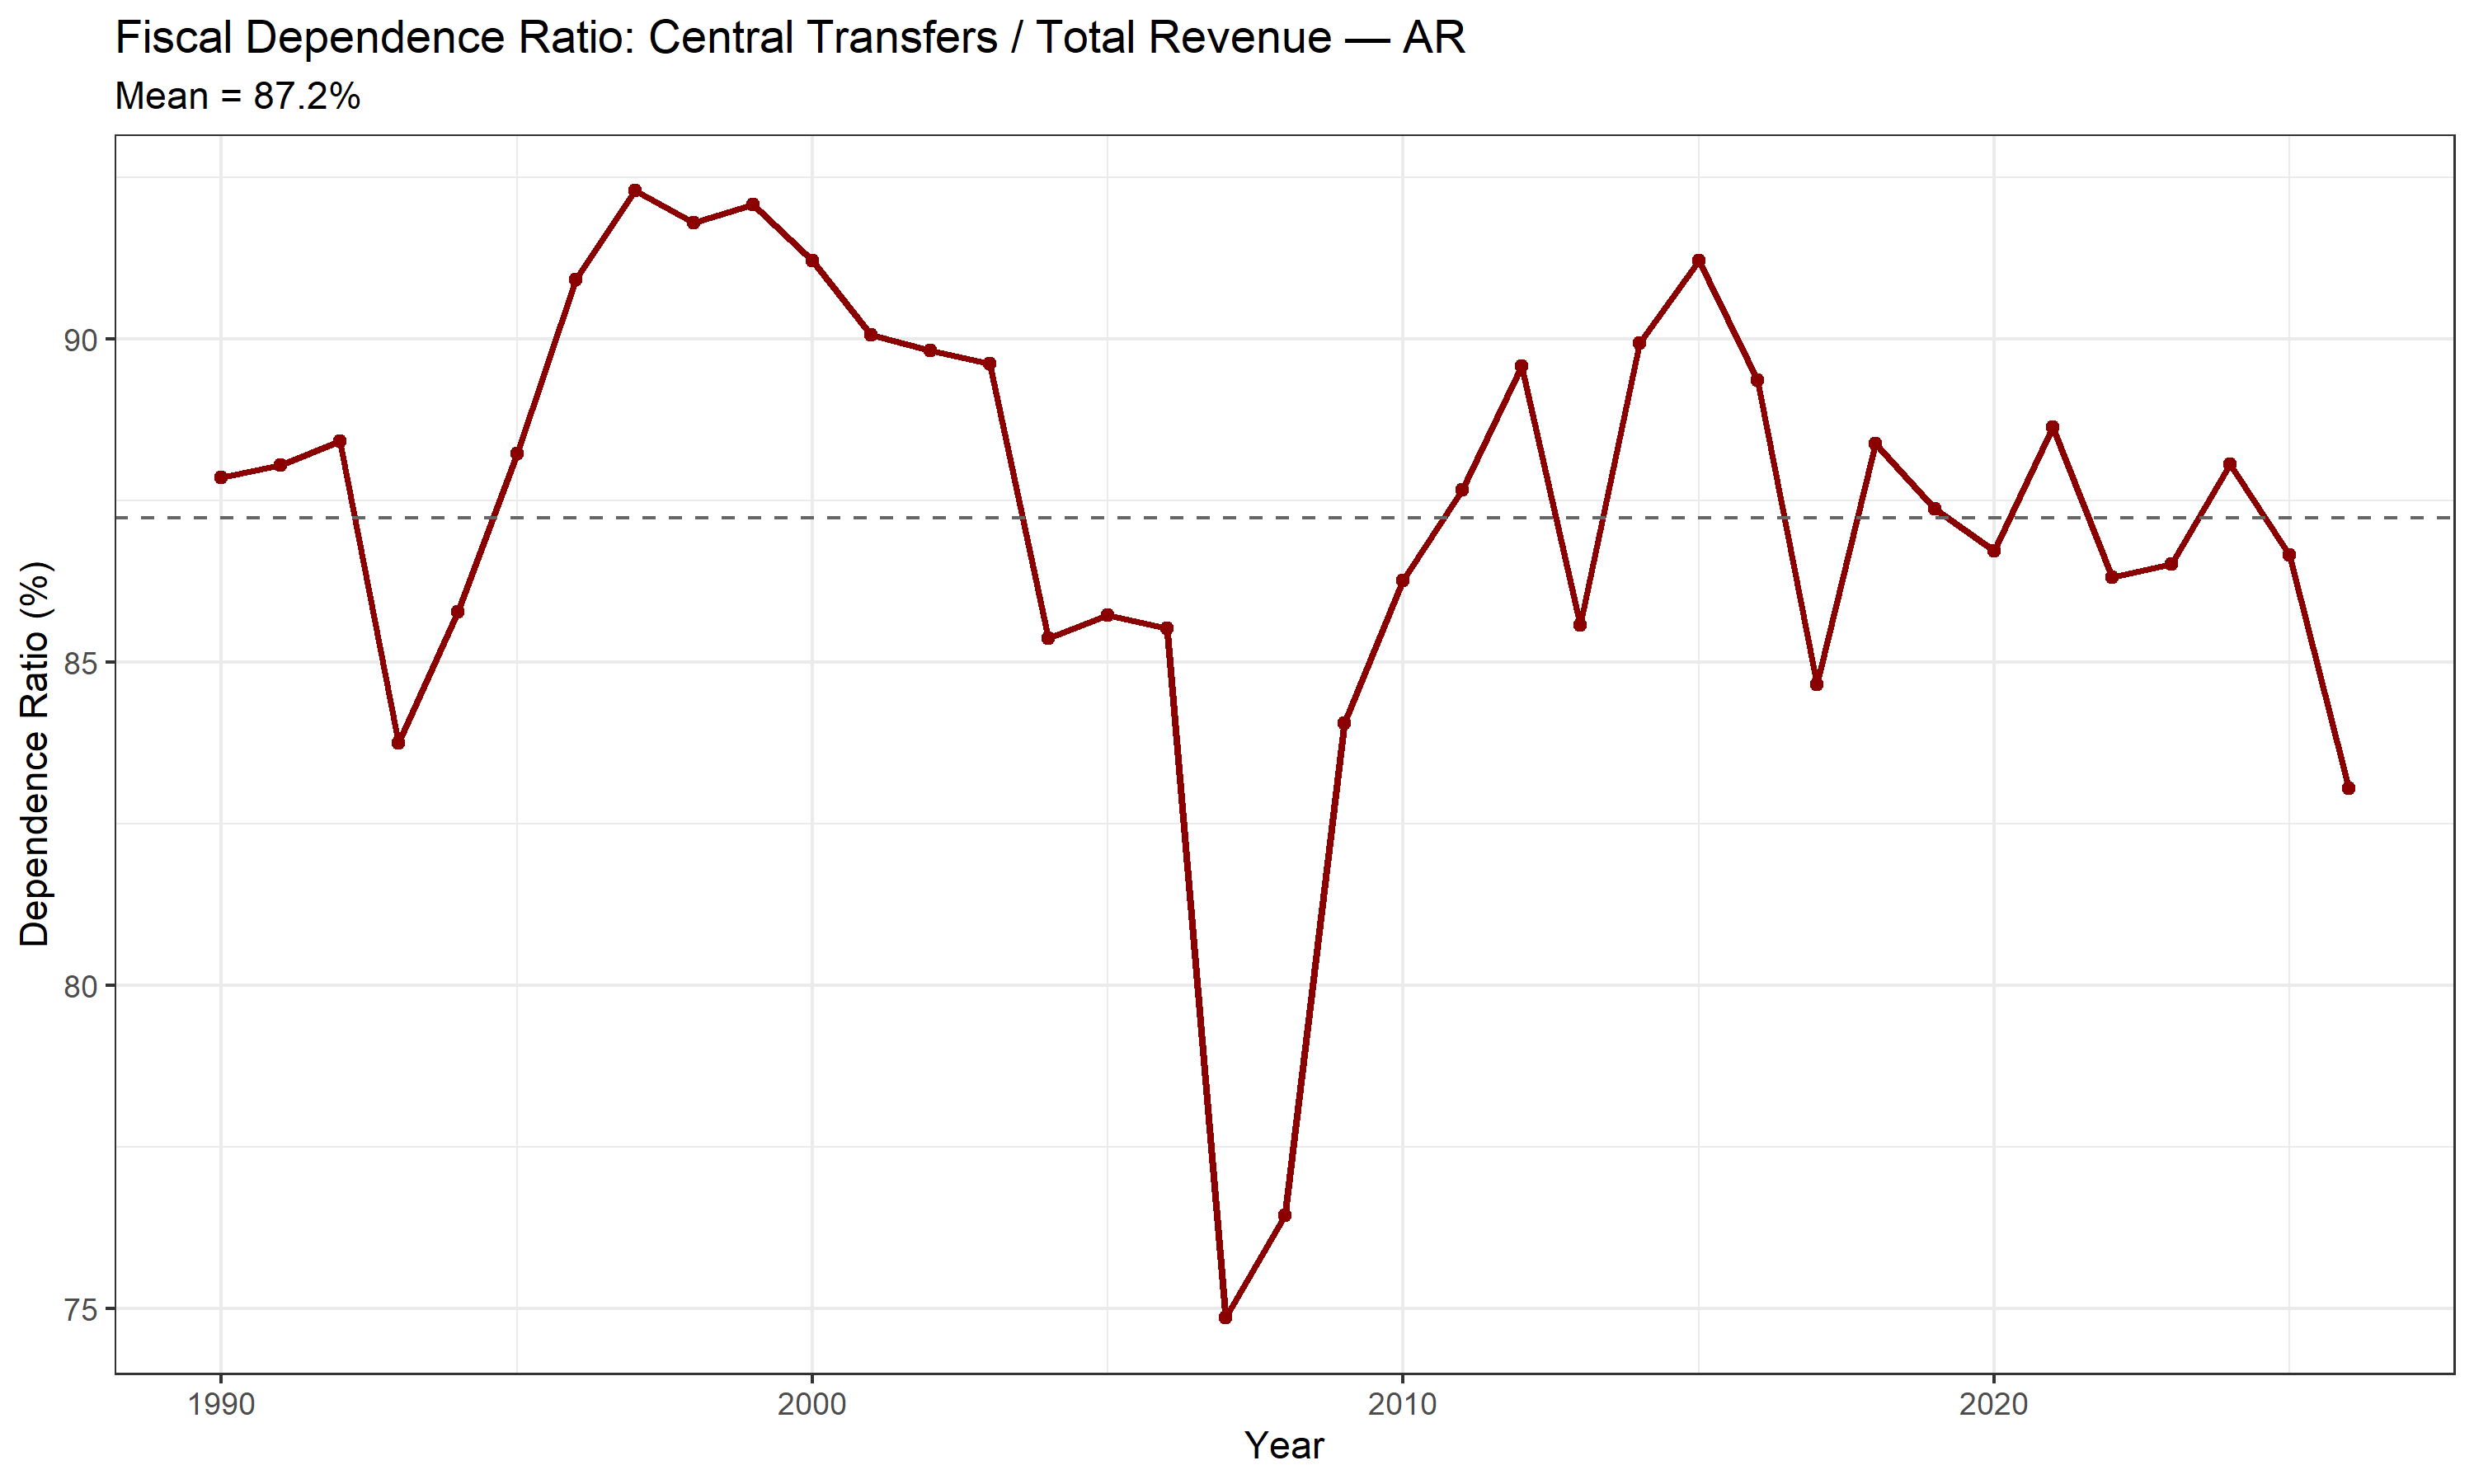
\includegraphics[width=0.92\textwidth]{fig8_fiscal_dependence.png}
\caption{Fiscal dependence ratio: related context}
\label{fig:fiscal-dependence}
\end{figure}

\begin{figure}[H]
\centering
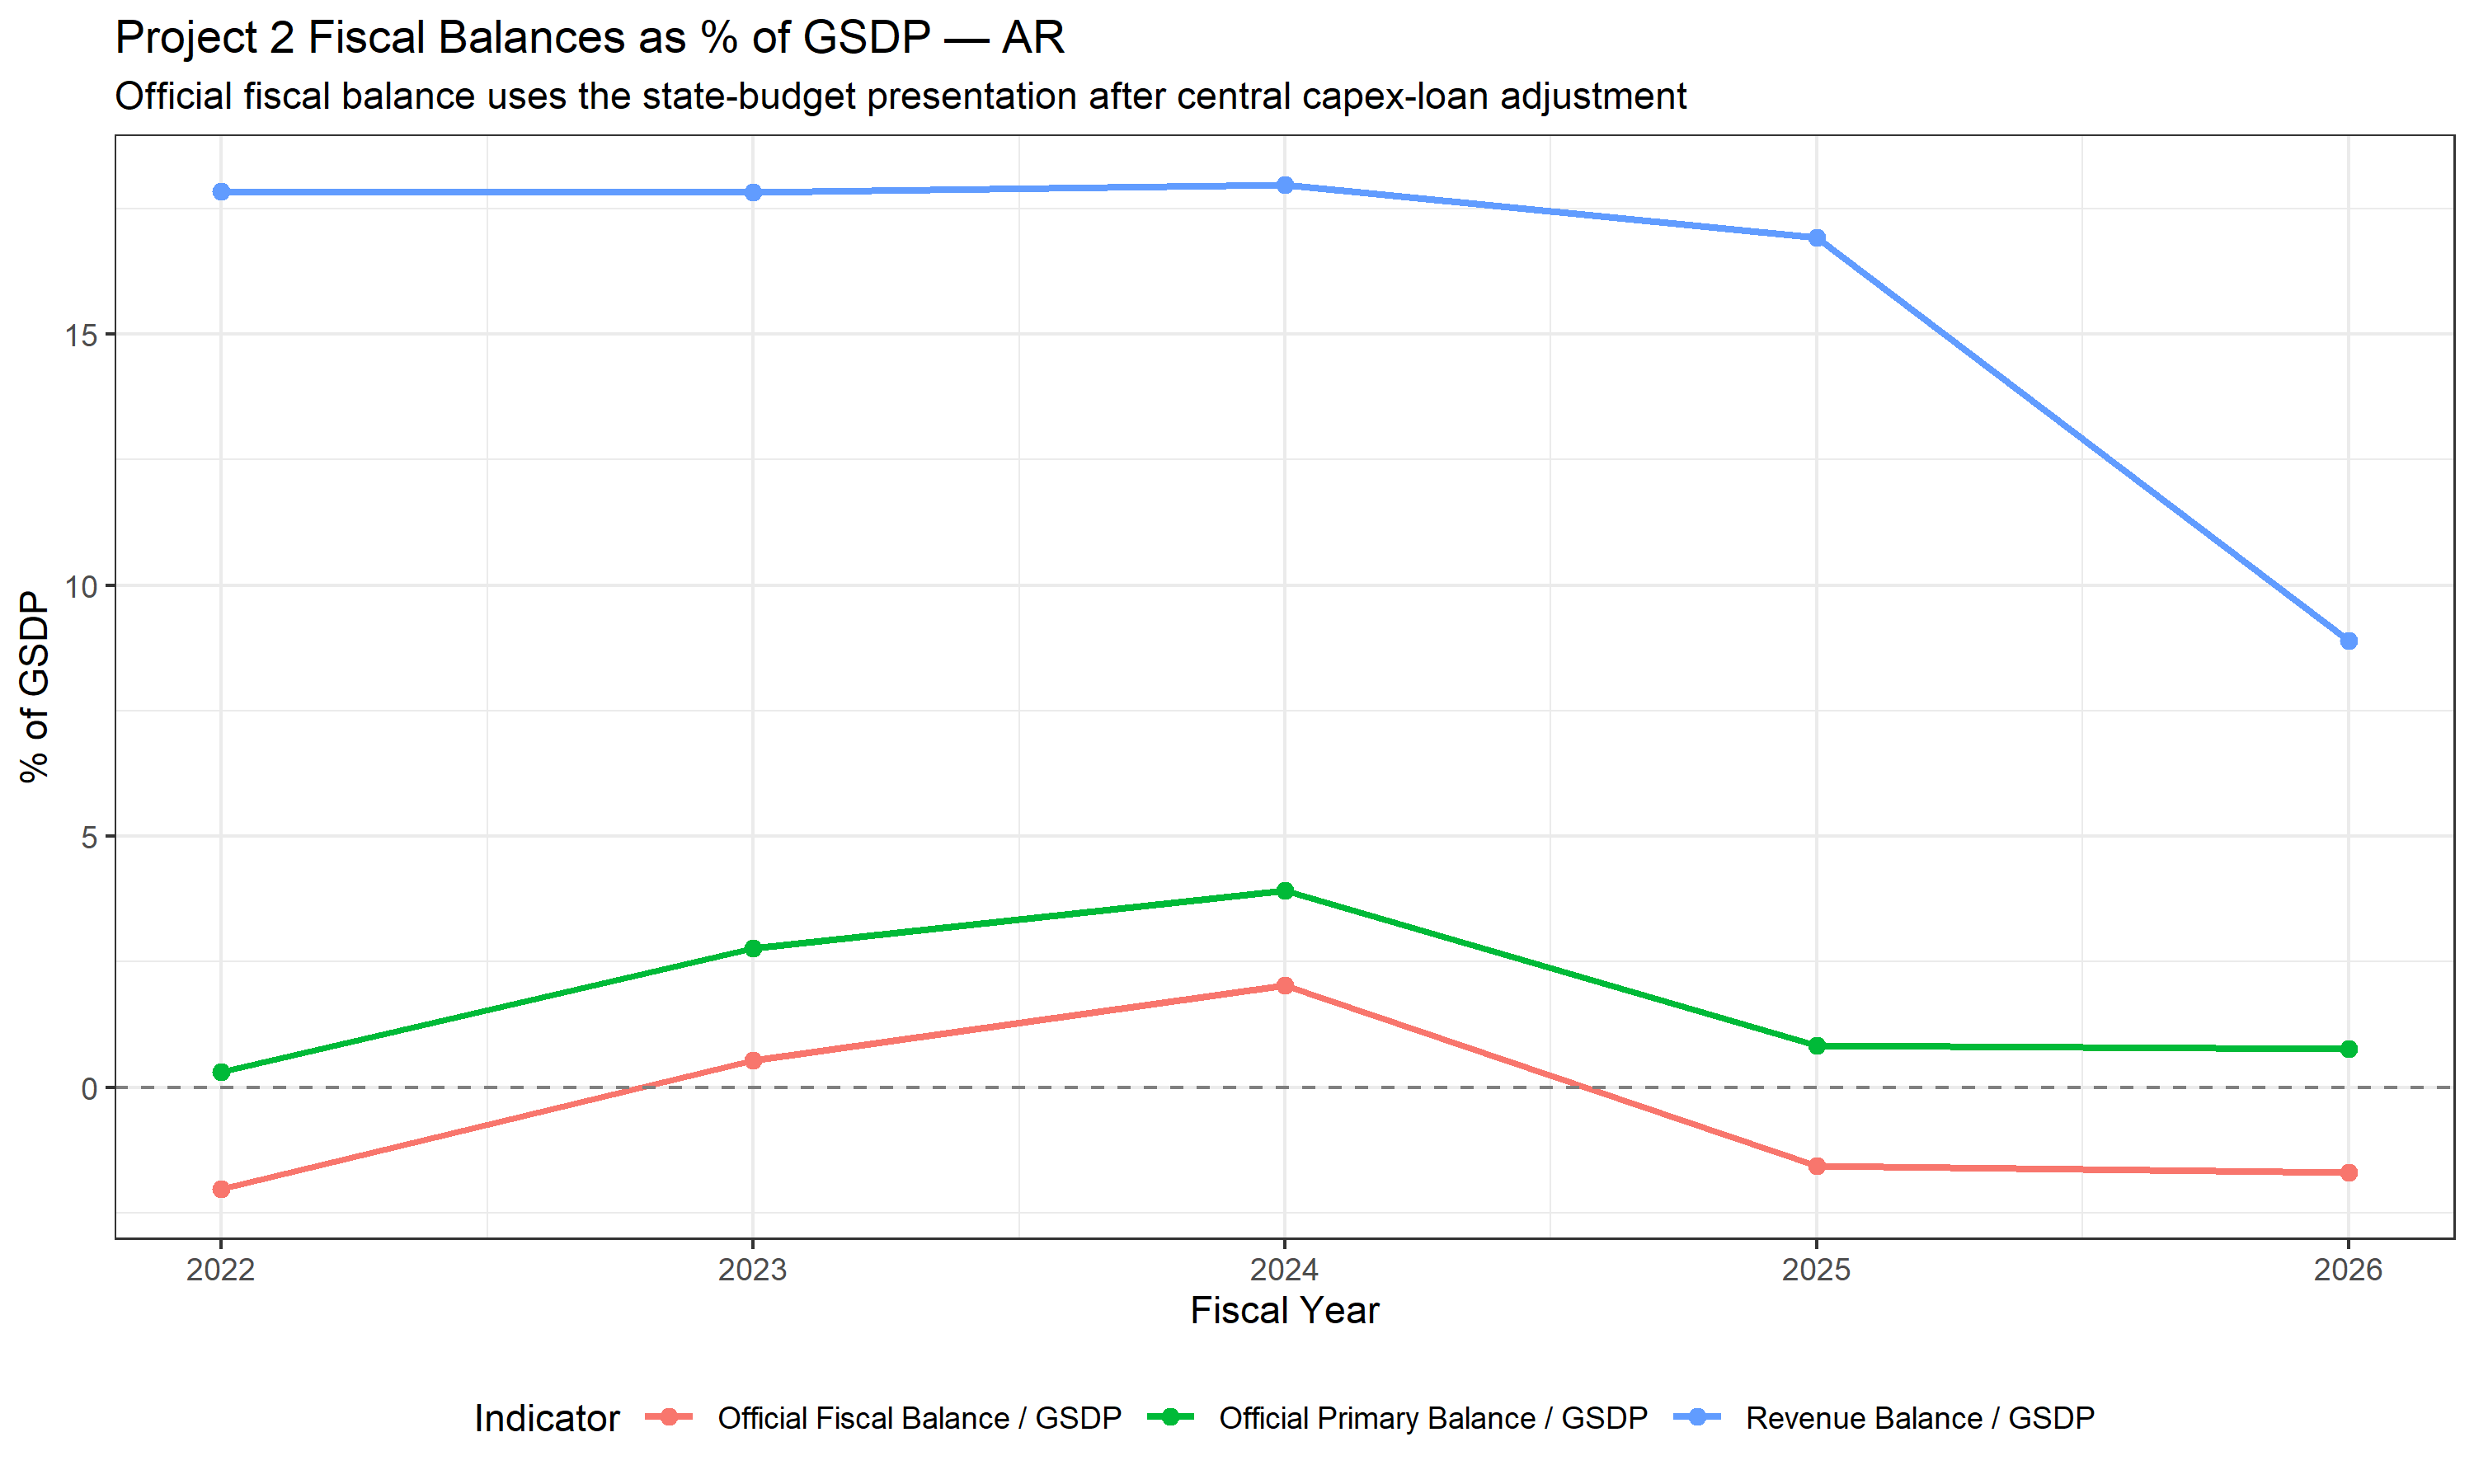
\includegraphics[width=0.92\textwidth]{fig9_fiscal_balances.png}
\caption{Fiscal balances as share of GSDP: related context}
\label{fig:fiscal-balances}
\end{figure}

\begin{figure}[H]
\centering
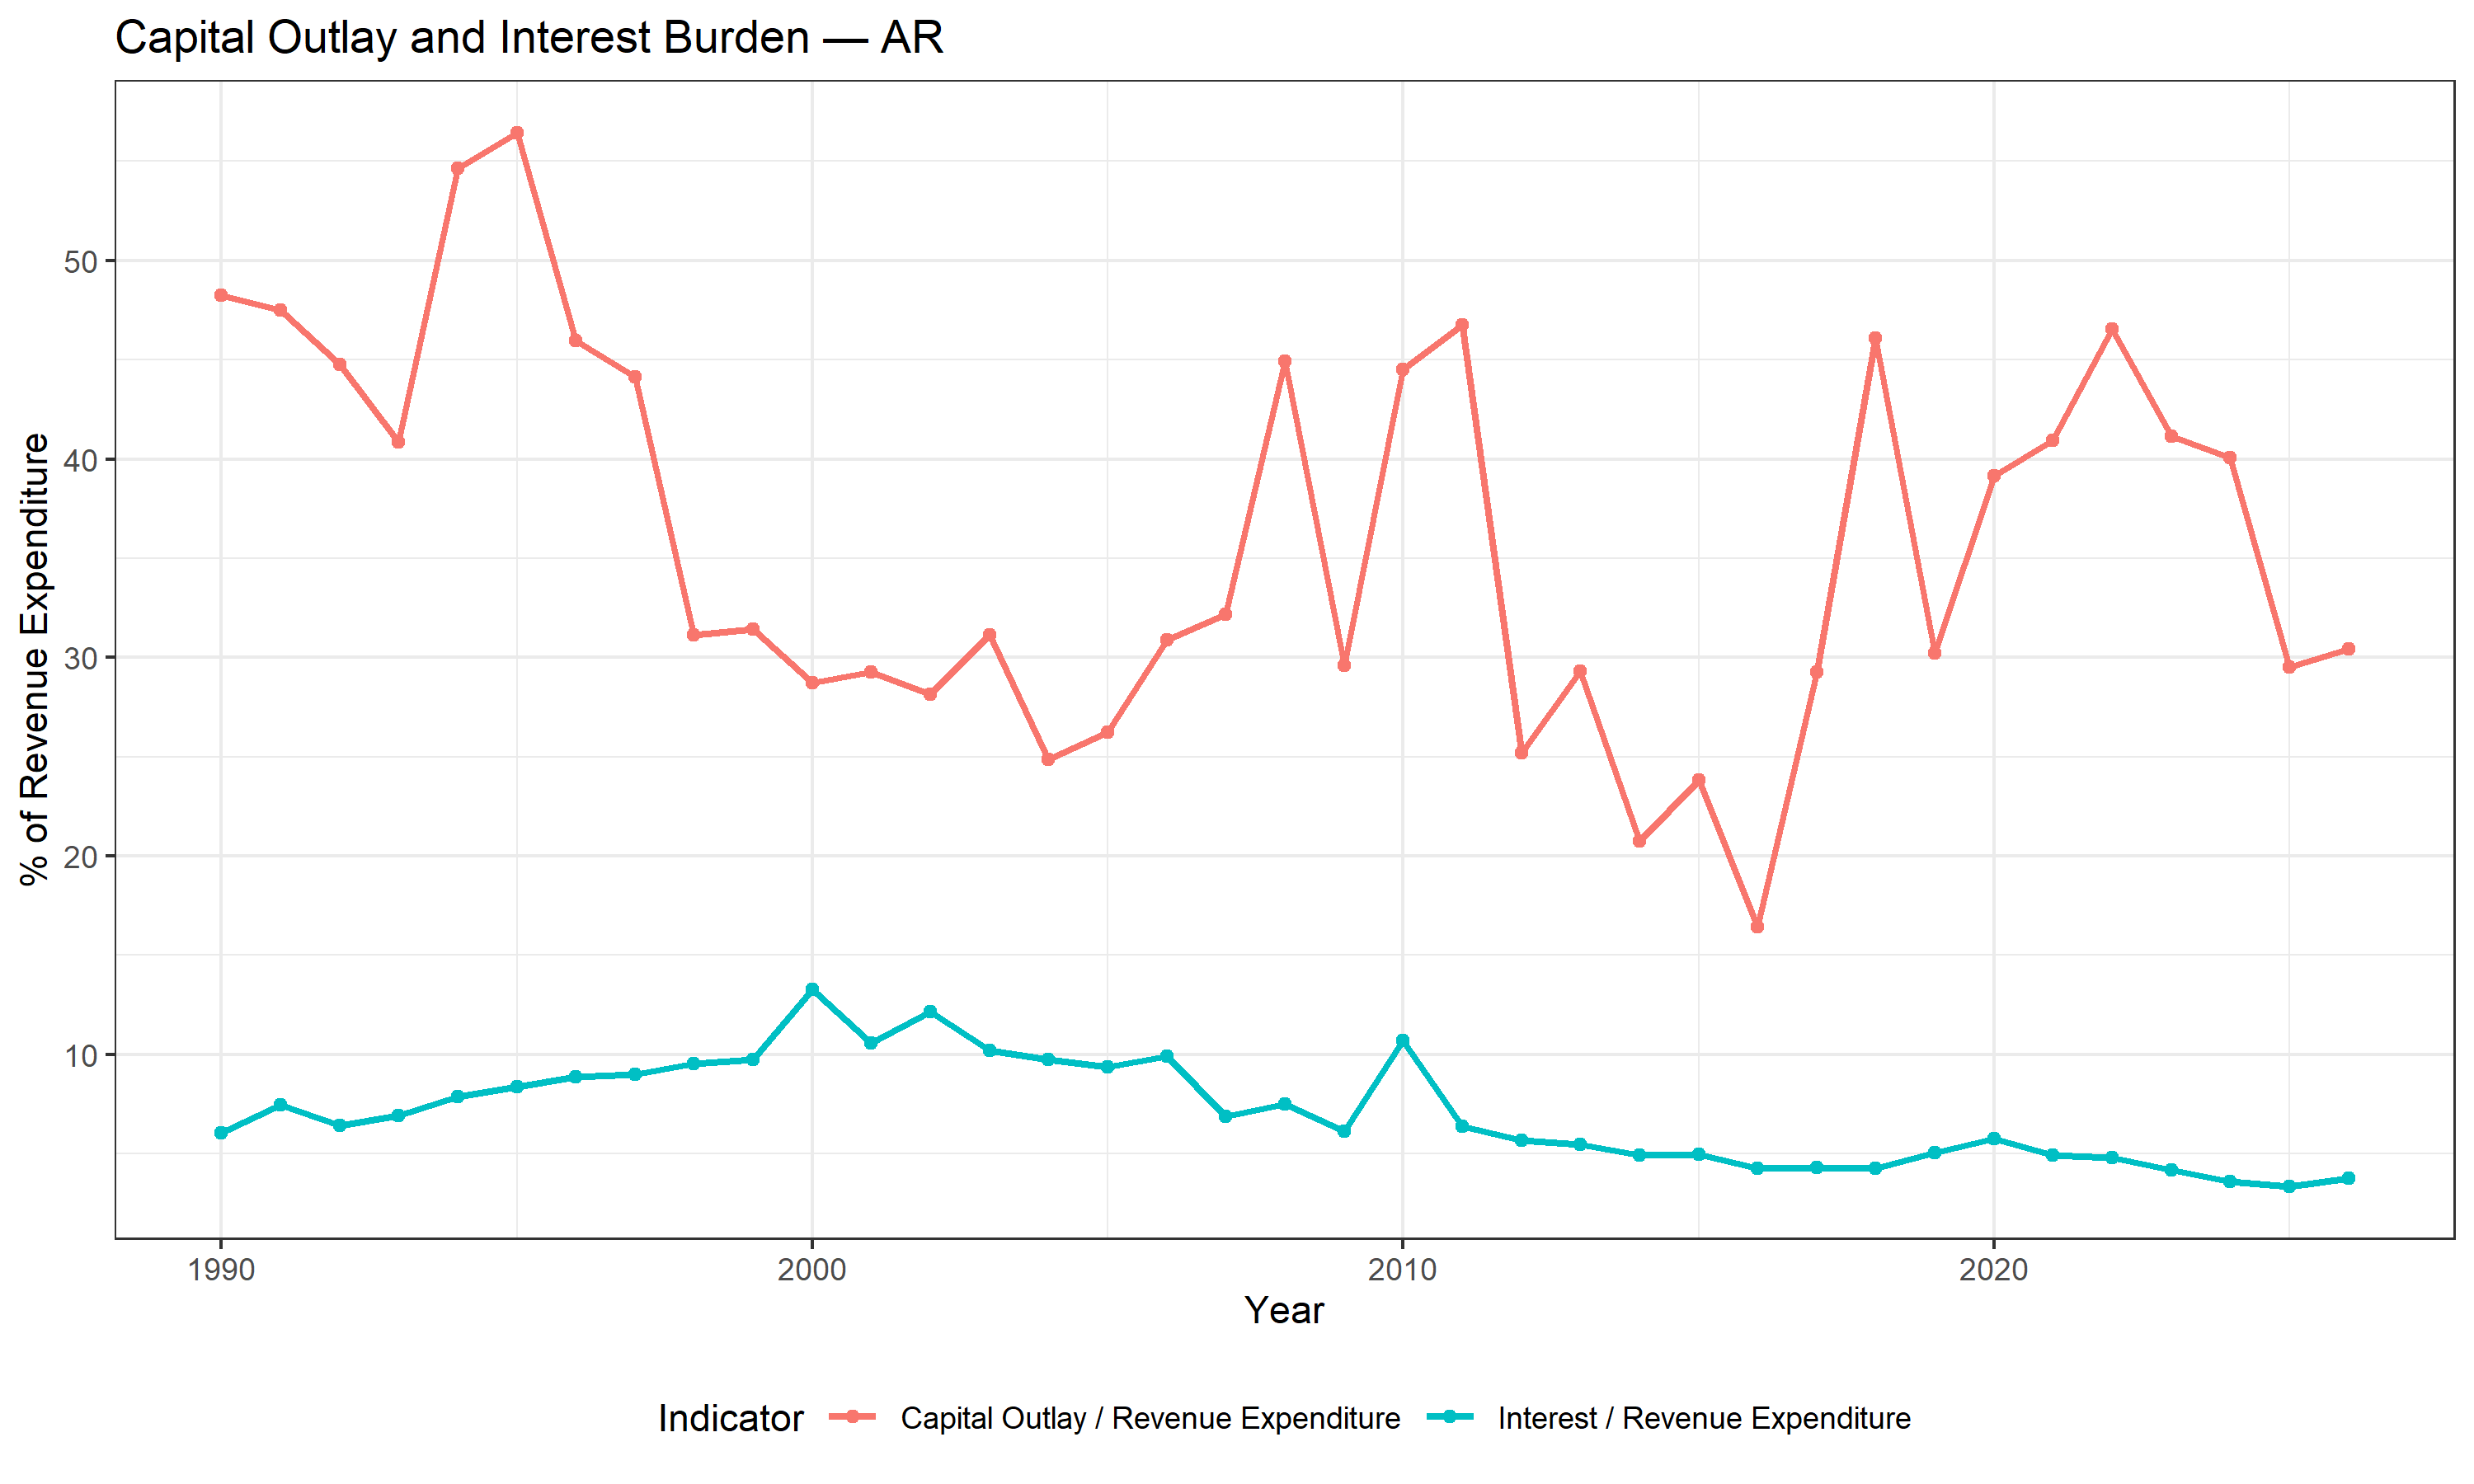
\includegraphics[width=0.92\textwidth]{fig10_interest_ratio.png}
\caption{Interest payments as share of revenue expenditure: related context}
\label{fig:interest}
\end{figure}

\begin{figure}[H]
\centering
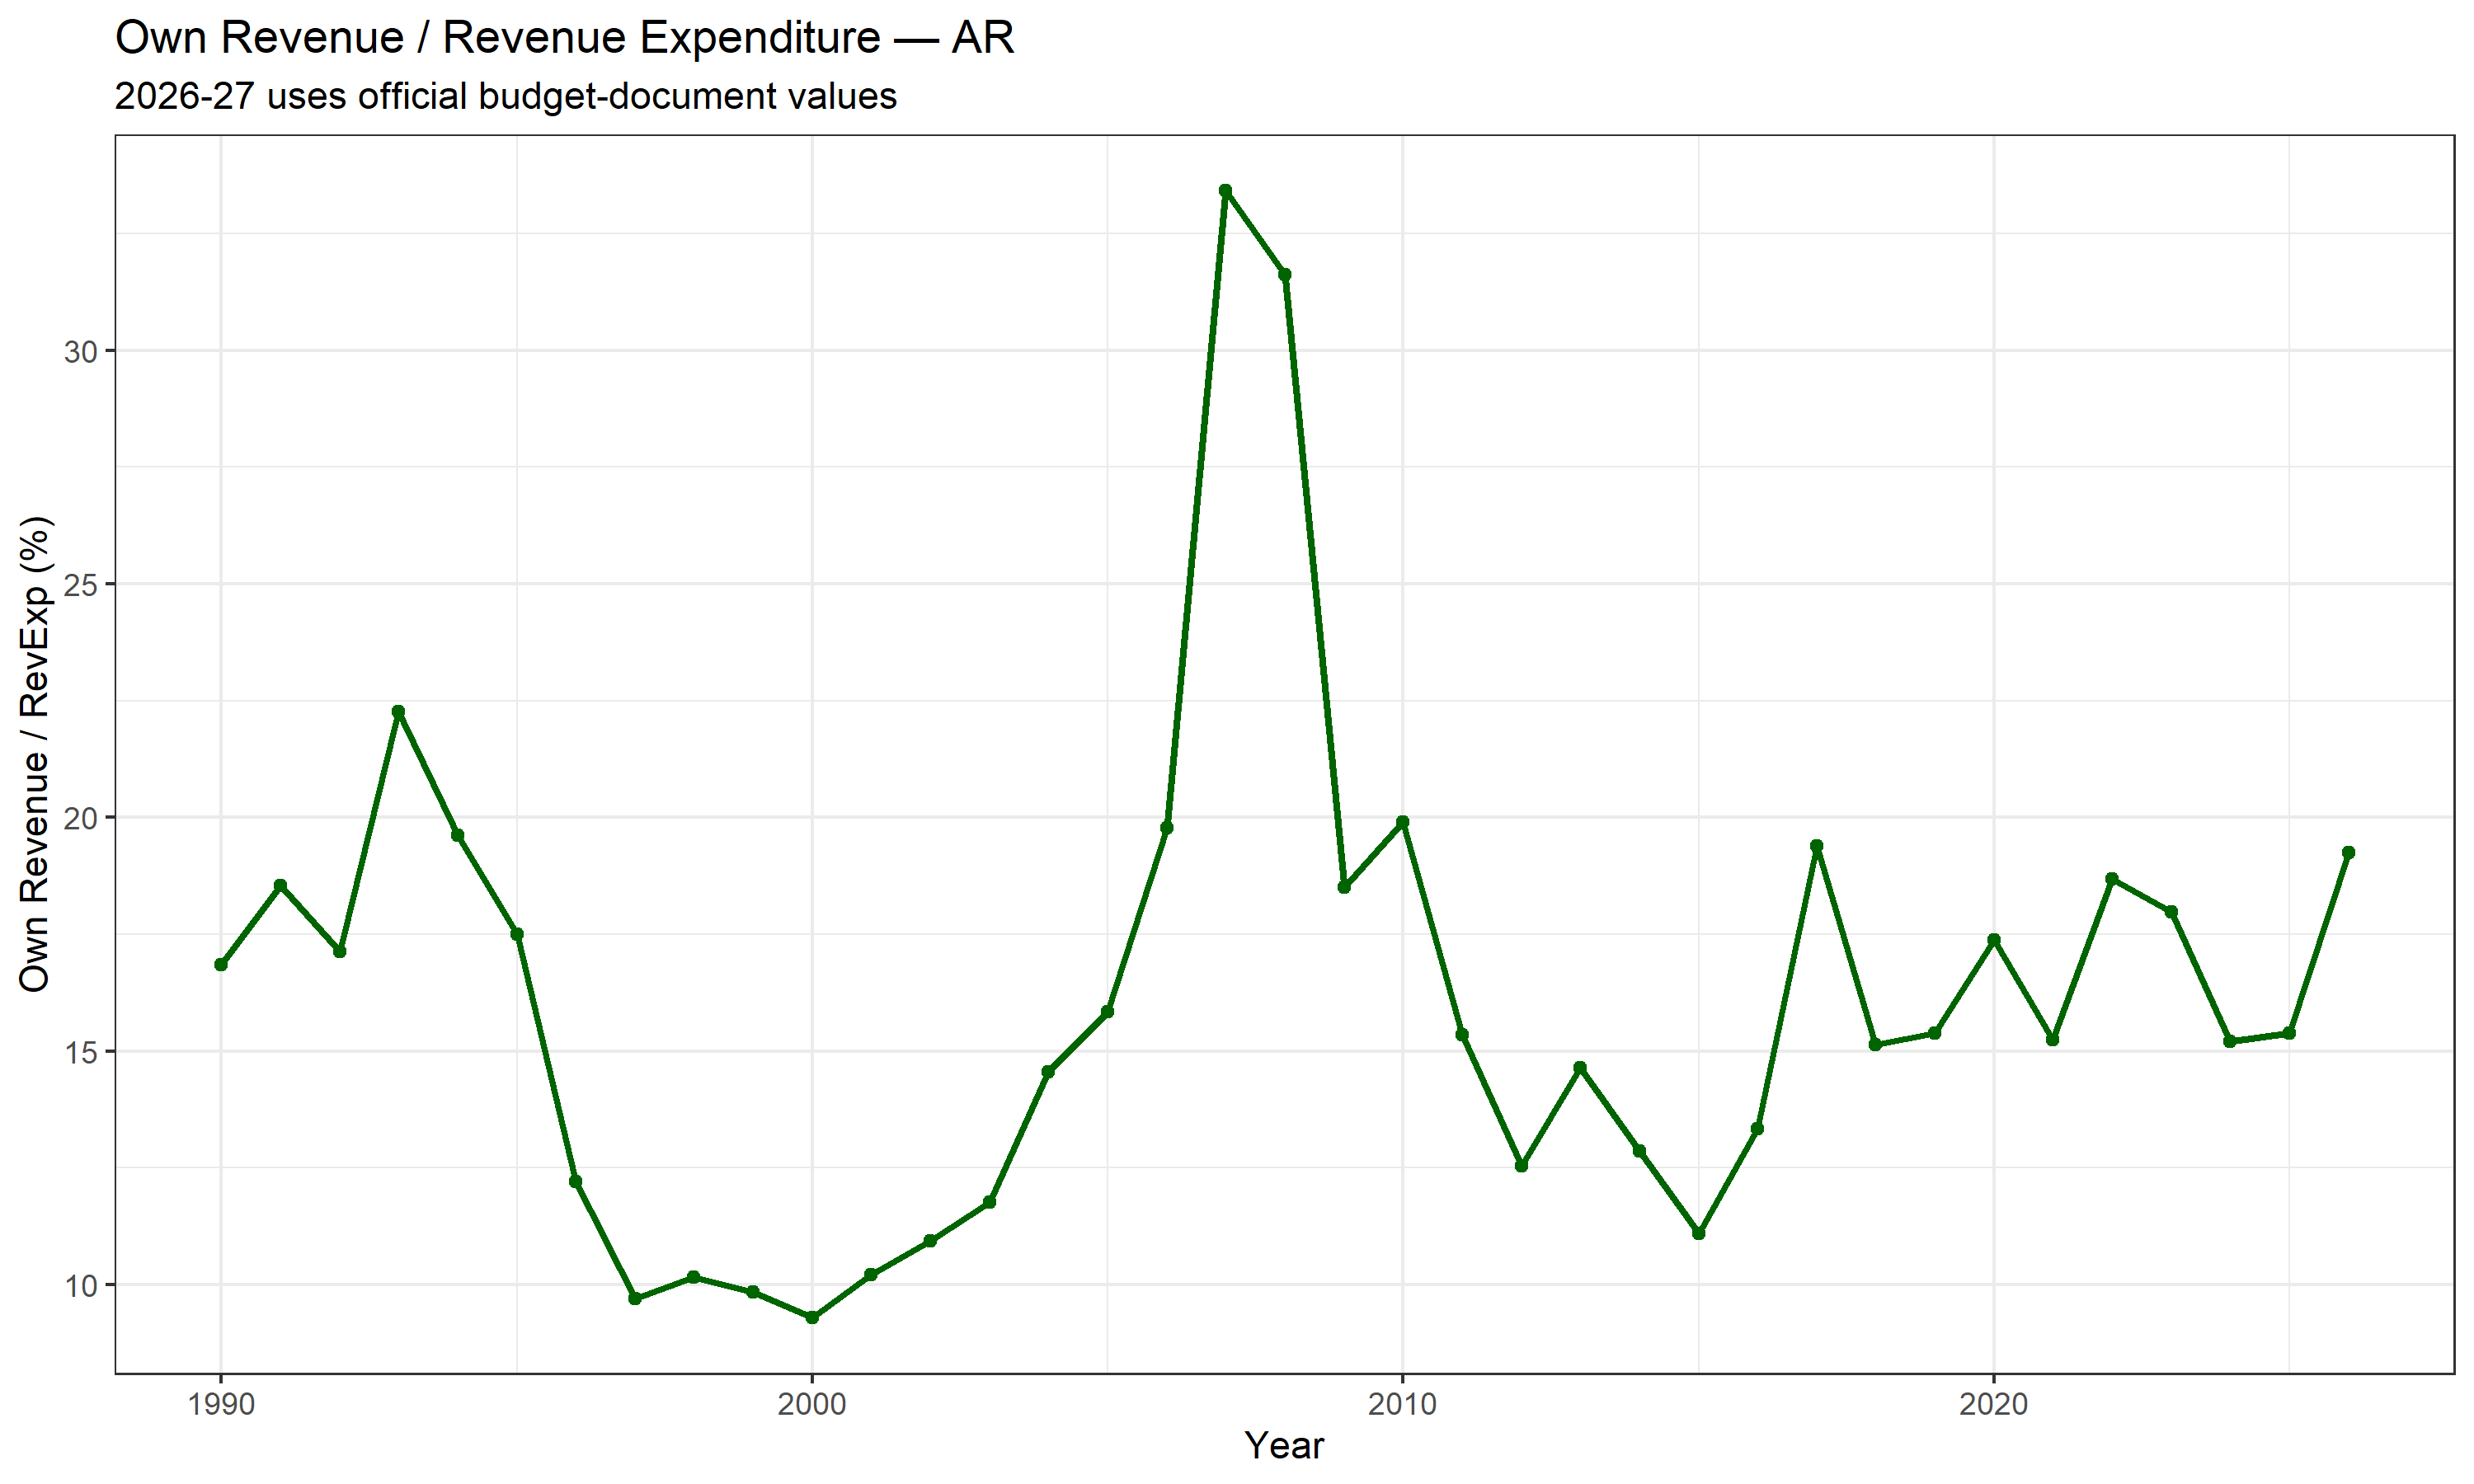
\includegraphics[width=0.92\textwidth]{fig11_own_revenue_ratio.png}
\caption{Own revenue as share of revenue expenditure: related context}
\label{fig:own-revenue}
\end{figure}

\section{Data Limitations}

Several limitations shape interpretation. First, Arunachal Pradesh GSDP before February 1987 refers to the territory that became the state. Second, Arunachal Pradesh CPI is rural-only. Urban CPI is absent and combined CPI is not reliable, so the state inflation analysis cannot be a rural-urban combined index like all India. Third, the state CPI basket is available only at group level, and housing is absent from the rural CPI series; the core index is therefore narrower than all-India core inflation. Fourth, April and May 2020 CPI observations are missing for Arunachal Pradesh, affecting 2020-21 annual and quarterly calculations. Fifth, quarterly GSDP deflator inflation is derived using Denton-Cholette interpolation from annual data, so the annual trend is reliable but sub-annual deflator movement should not be over-interpreted. Sixth, annual fiscal-year inflation effectively starts in 2012-13 because the monthly CPI panel begins only in January 2011, leaving no full 2010-11 fiscal-year baseline for a 2011-12 year-on-year calculation. Seventh, cross-state headline, food, and fuel inflation can be computed from the published combined CPI indices, but an exact combined-state core inflation measure is not reported because the available state weight file provides rural and urban basket weights rather than a state-specific combined basket weight vector.

\bibliographystyle{apalike}
\bibliography{references}

\end{document}
